%% m4l vs pt4l
\begin{figure}[H]
    \begin{subfigure}{.46\textwidth}\centering
      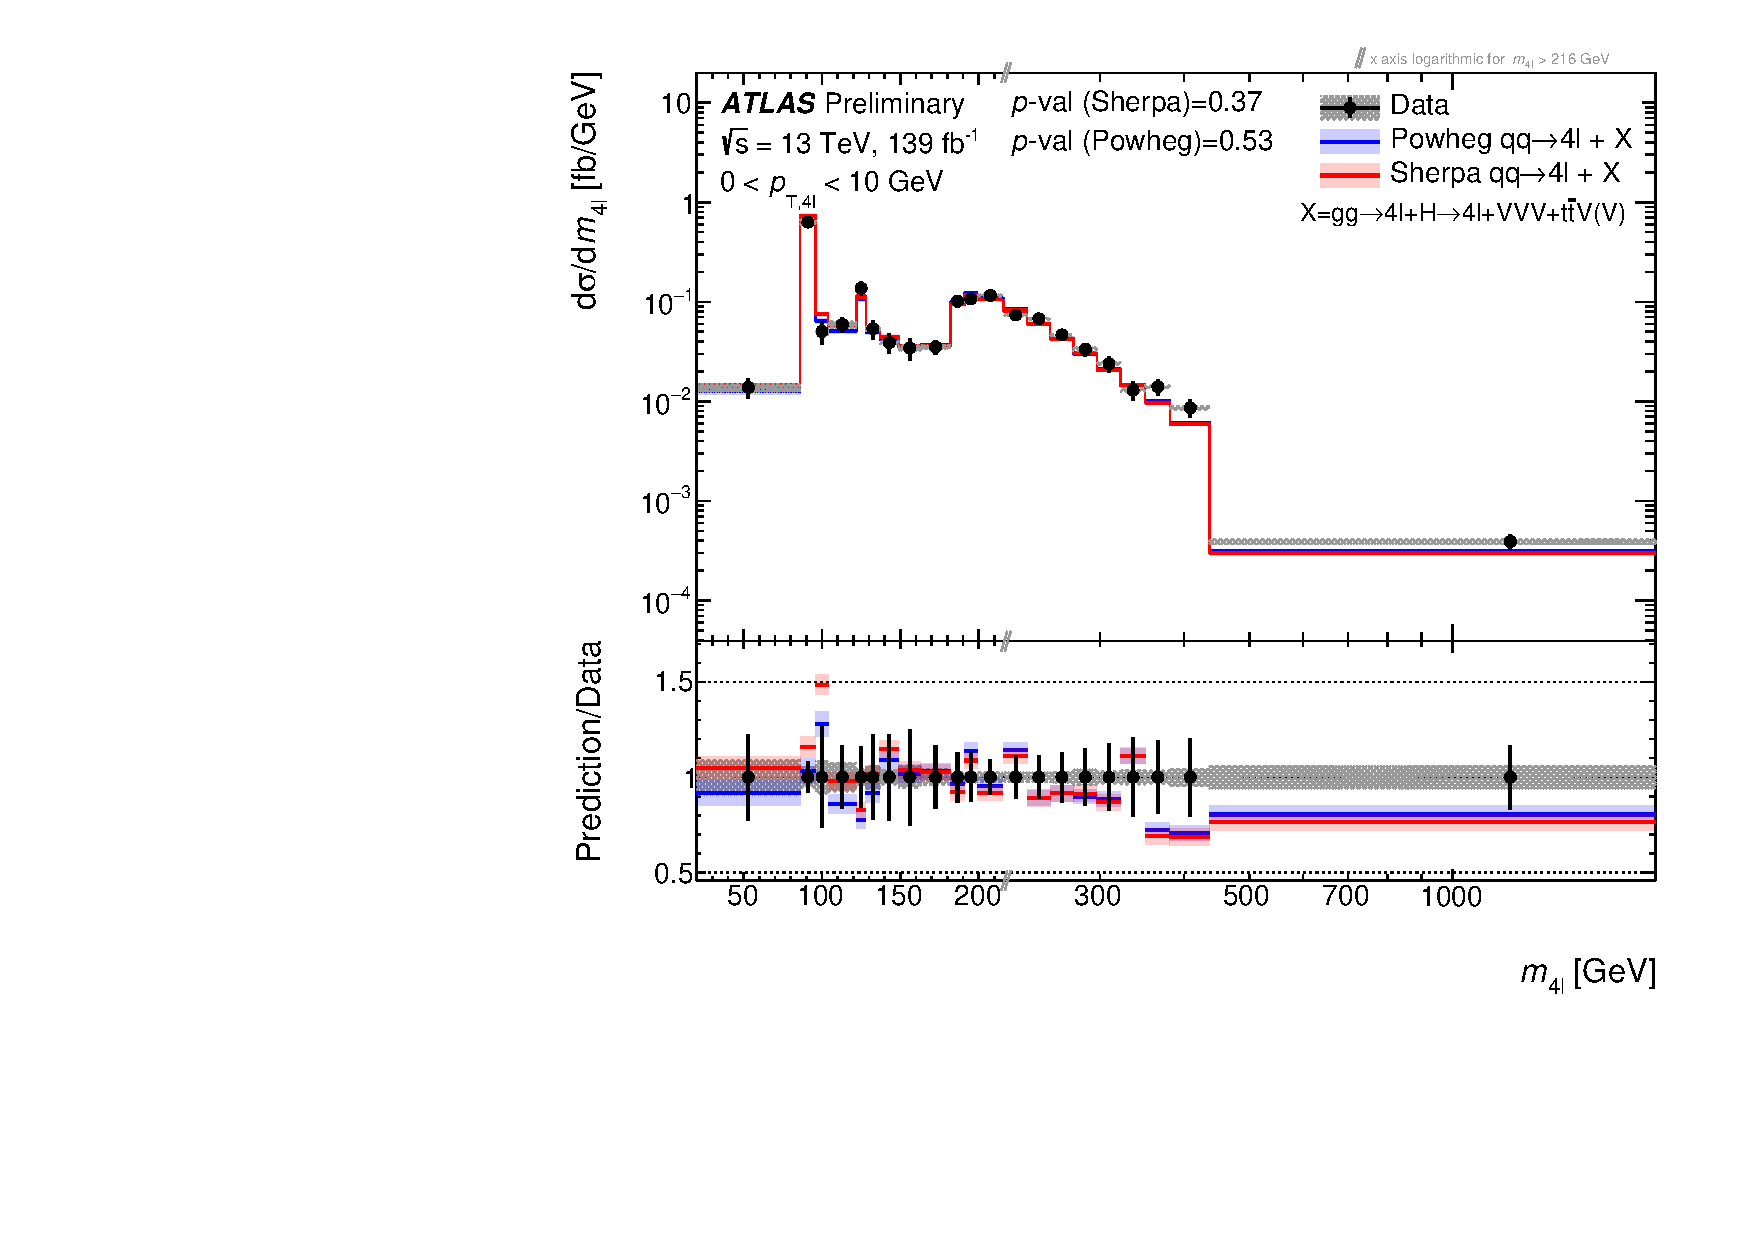
\includegraphics[width=.95\linewidth]{Figures/m4l/UnfoldedResults/linlog_Unfolded_Data_m4l_pt4l0-10.pdf}\caption{$\unit{0}{\GeV} <  \ptFourL  < \unit{10}{\GeV}$}\label{fig:sub-first}
    \end{subfigure}
    \begin{subfigure}{.46\textwidth}\centering
      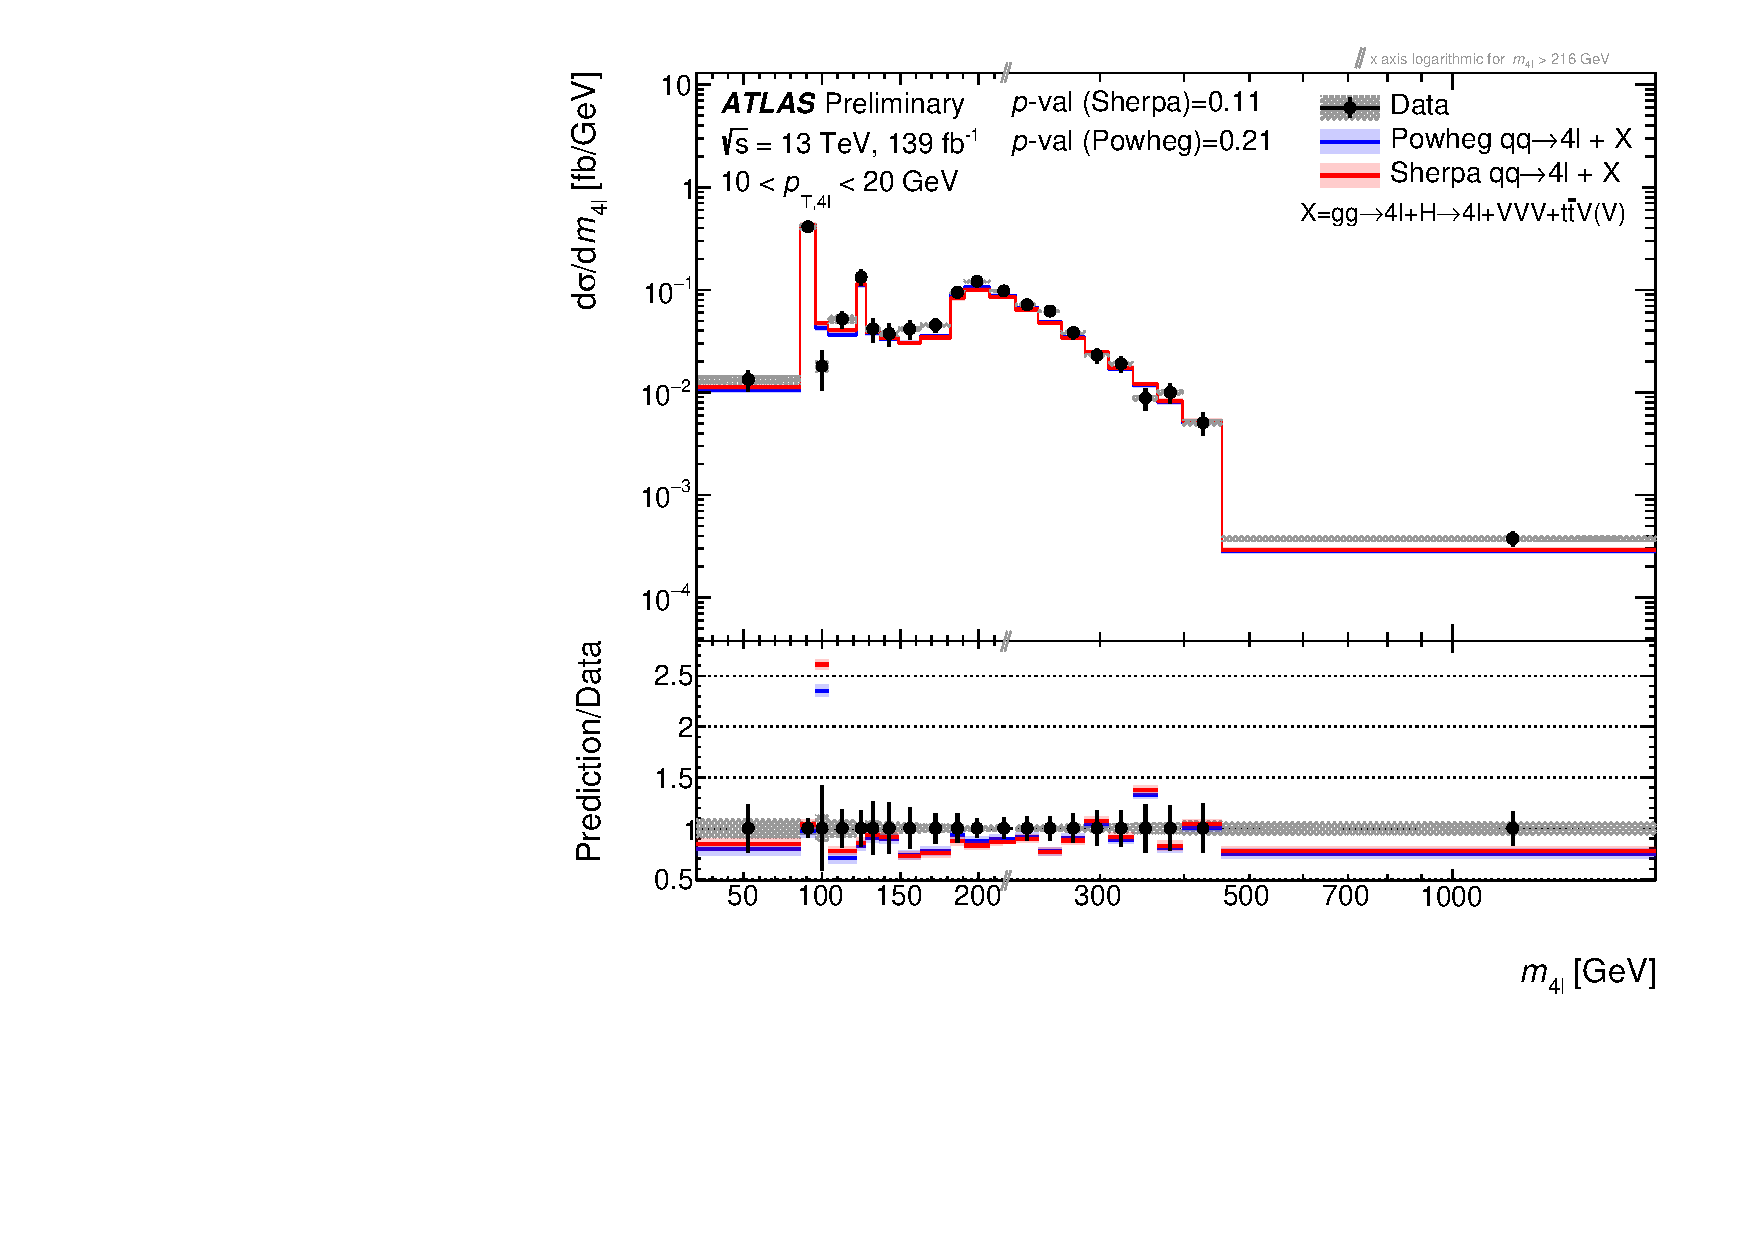
\includegraphics[width=.95\linewidth]{Figures/m4l/UnfoldedResults/linlog_Unfolded_Data_m4l_pt4l10-20.pdf} \caption{$\unit{10}{\GeV} <  \ptFourL  < \unit{20}{\GeV}$}\label{fig:sub-second}
    \end{subfigure}
    \begin{subfigure}{.46\textwidth}\centering
      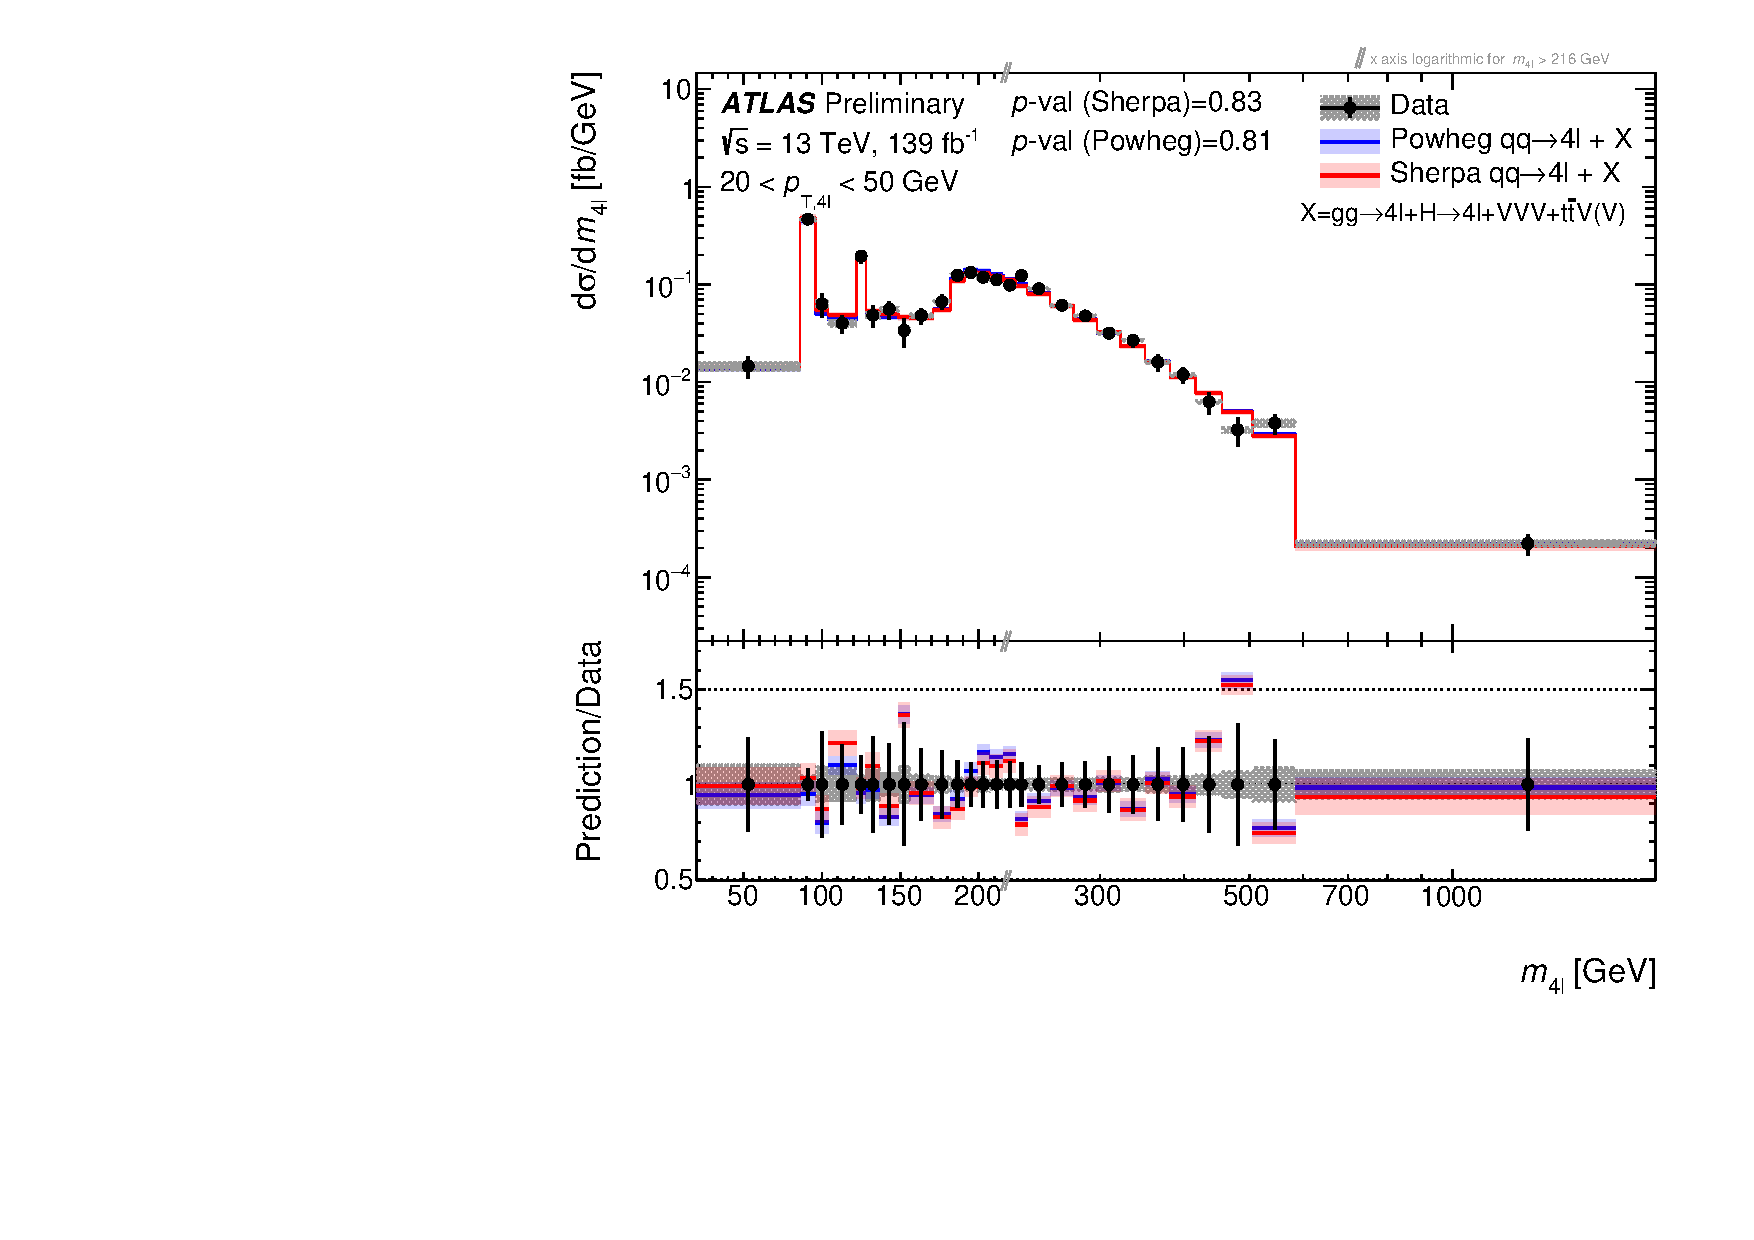
\includegraphics[width=.95\linewidth]{Figures/m4l/UnfoldedResults/linlog_Unfolded_Data_m4l_pt4l20-50.pdf}  \caption{$\unit{20}{\GeV} <  \ptFourL  < \unit{50}{\GeV}$}\label{fig:sub-third}
    \end{subfigure}
    \begin{subfigure}{.46\textwidth}\centering
      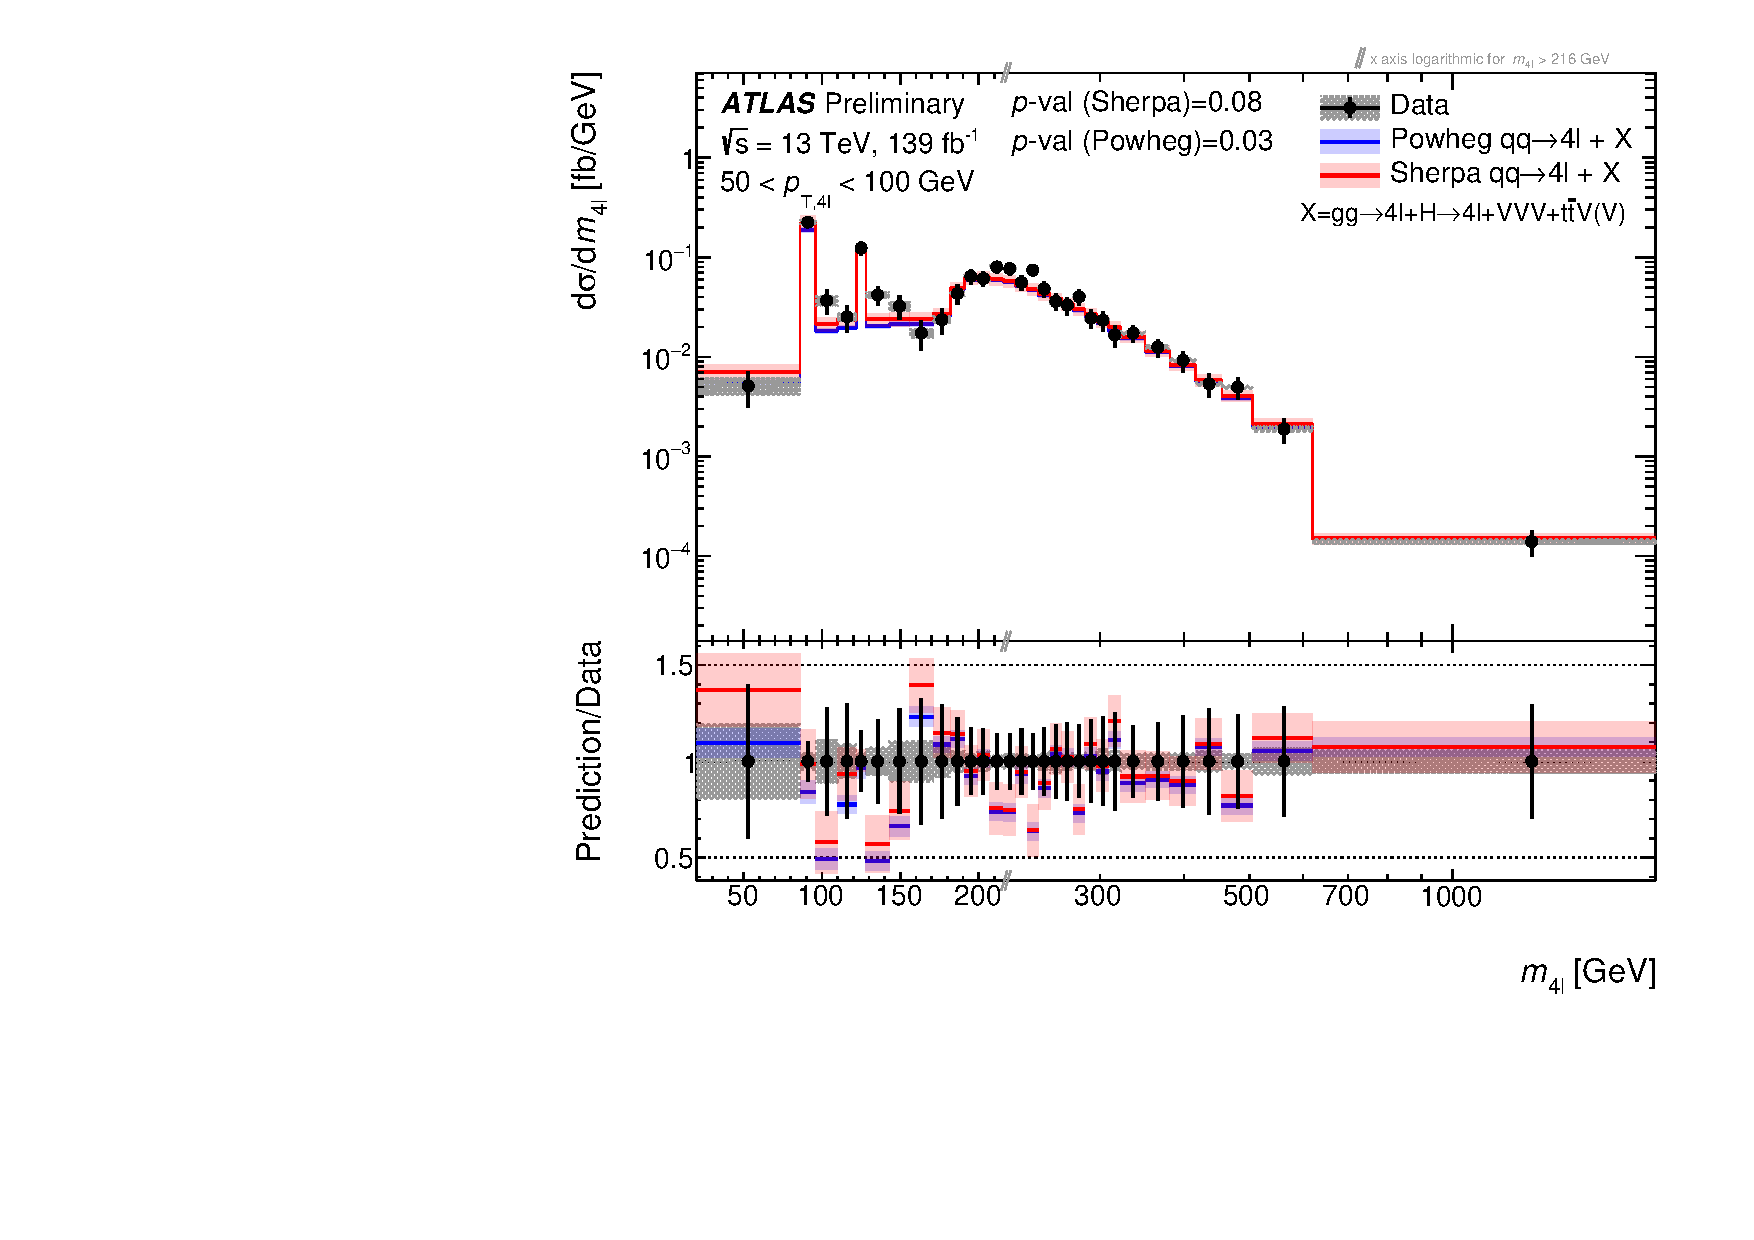
\includegraphics[width=.95\linewidth]{Figures/m4l/UnfoldedResults/linlog_Unfolded_Data_m4l_pt4l50-100.pdf}  \caption{$\unit{50}{\GeV} <  \ptFourL  < \unit{100}{\GeV}$}\label{fig:sub-fourth}
    \end{subfigure}
        \begin{subfigure}{.46\textwidth}\centering
      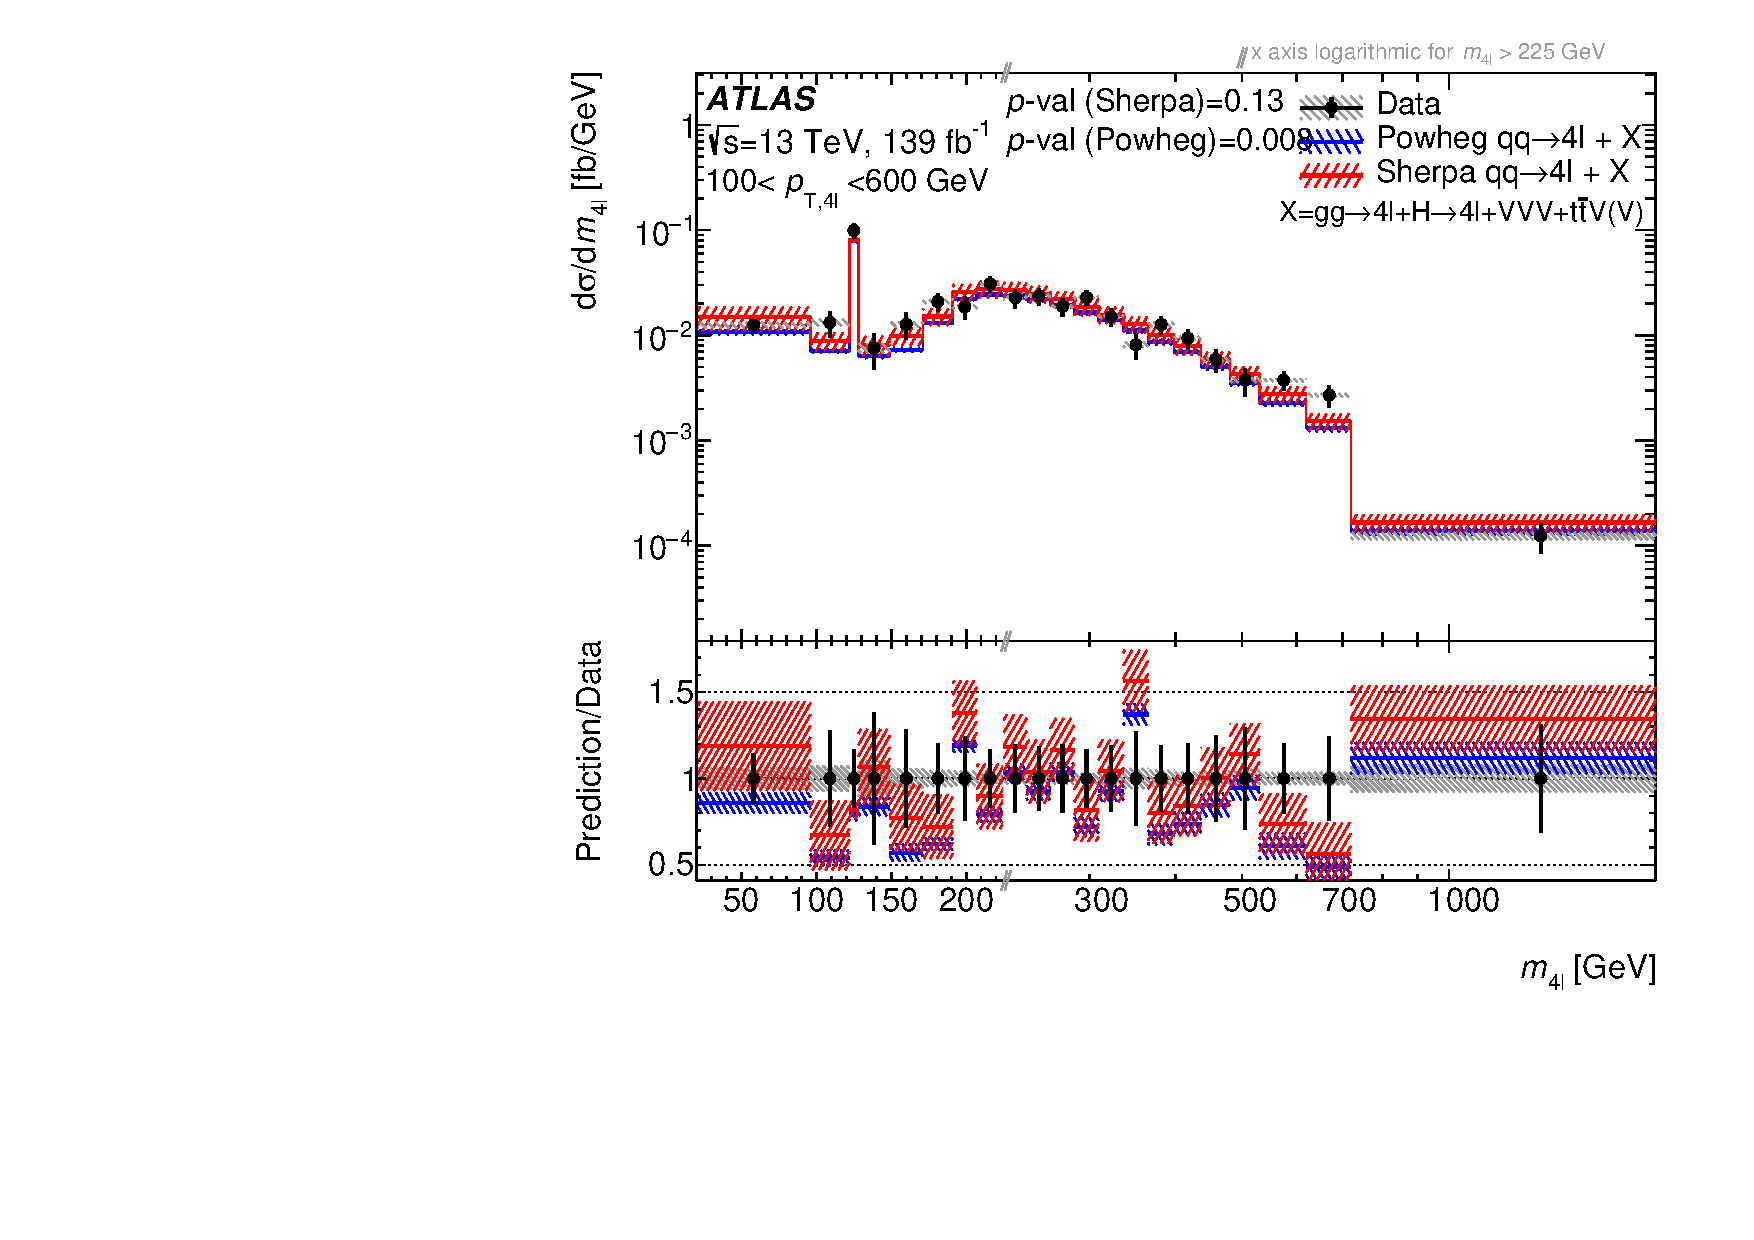
\includegraphics[width=.95\linewidth]{Figures/m4l/UnfoldedResults/linlog_Unfolded_Data_m4l_pt4l100-600.pdf}  \caption{$\unit{100}{\GeV} <  \ptFourL  < \unit{60 0}{\GeV}$}\label{fig:sub-fifth}
    \end{subfigure}
    \caption{Differential cross-section as a function of \mFourL{} in slices of \ptFourL{}. \errorbars{} \SMpredictions{} \Pvalue{} The ratio of the \SHERPA{} prediction to the data is shown in the lower panel.}
    \label{fig:m4l_pt4l}
\end{figure}

%% m4l vs y4l
\begin{figure}[H]
    \begin{subfigure}{.46\textwidth}\centering
      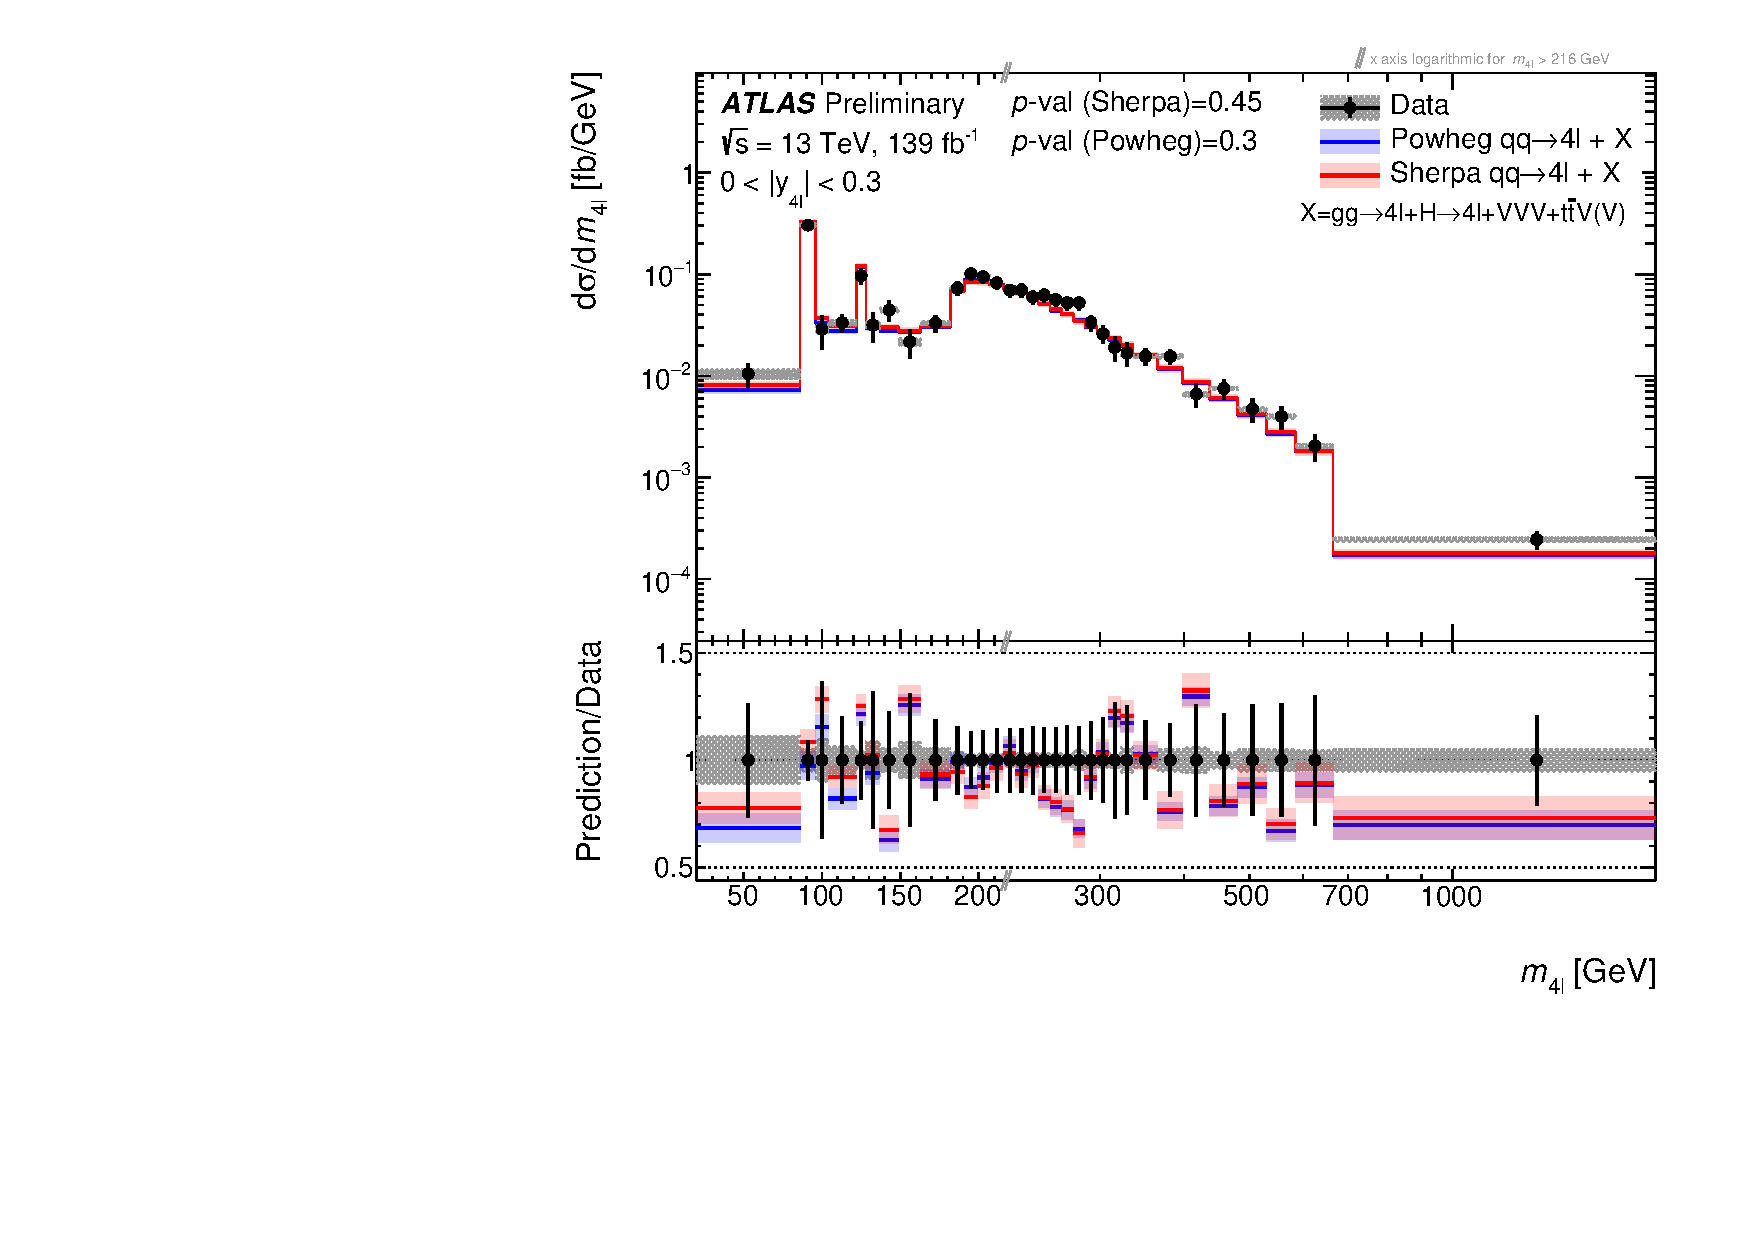
\includegraphics[width=.95\linewidth]{Figures/m4l/UnfoldedResults/linlog_Unfolded_Data_m4l_y4l0-0dot3.pdf}\caption{0 < \yFourL{} < 0.3}\label{fig:sub-first}
    \end{subfigure}
    \begin{subfigure}{.46\textwidth}\centering
      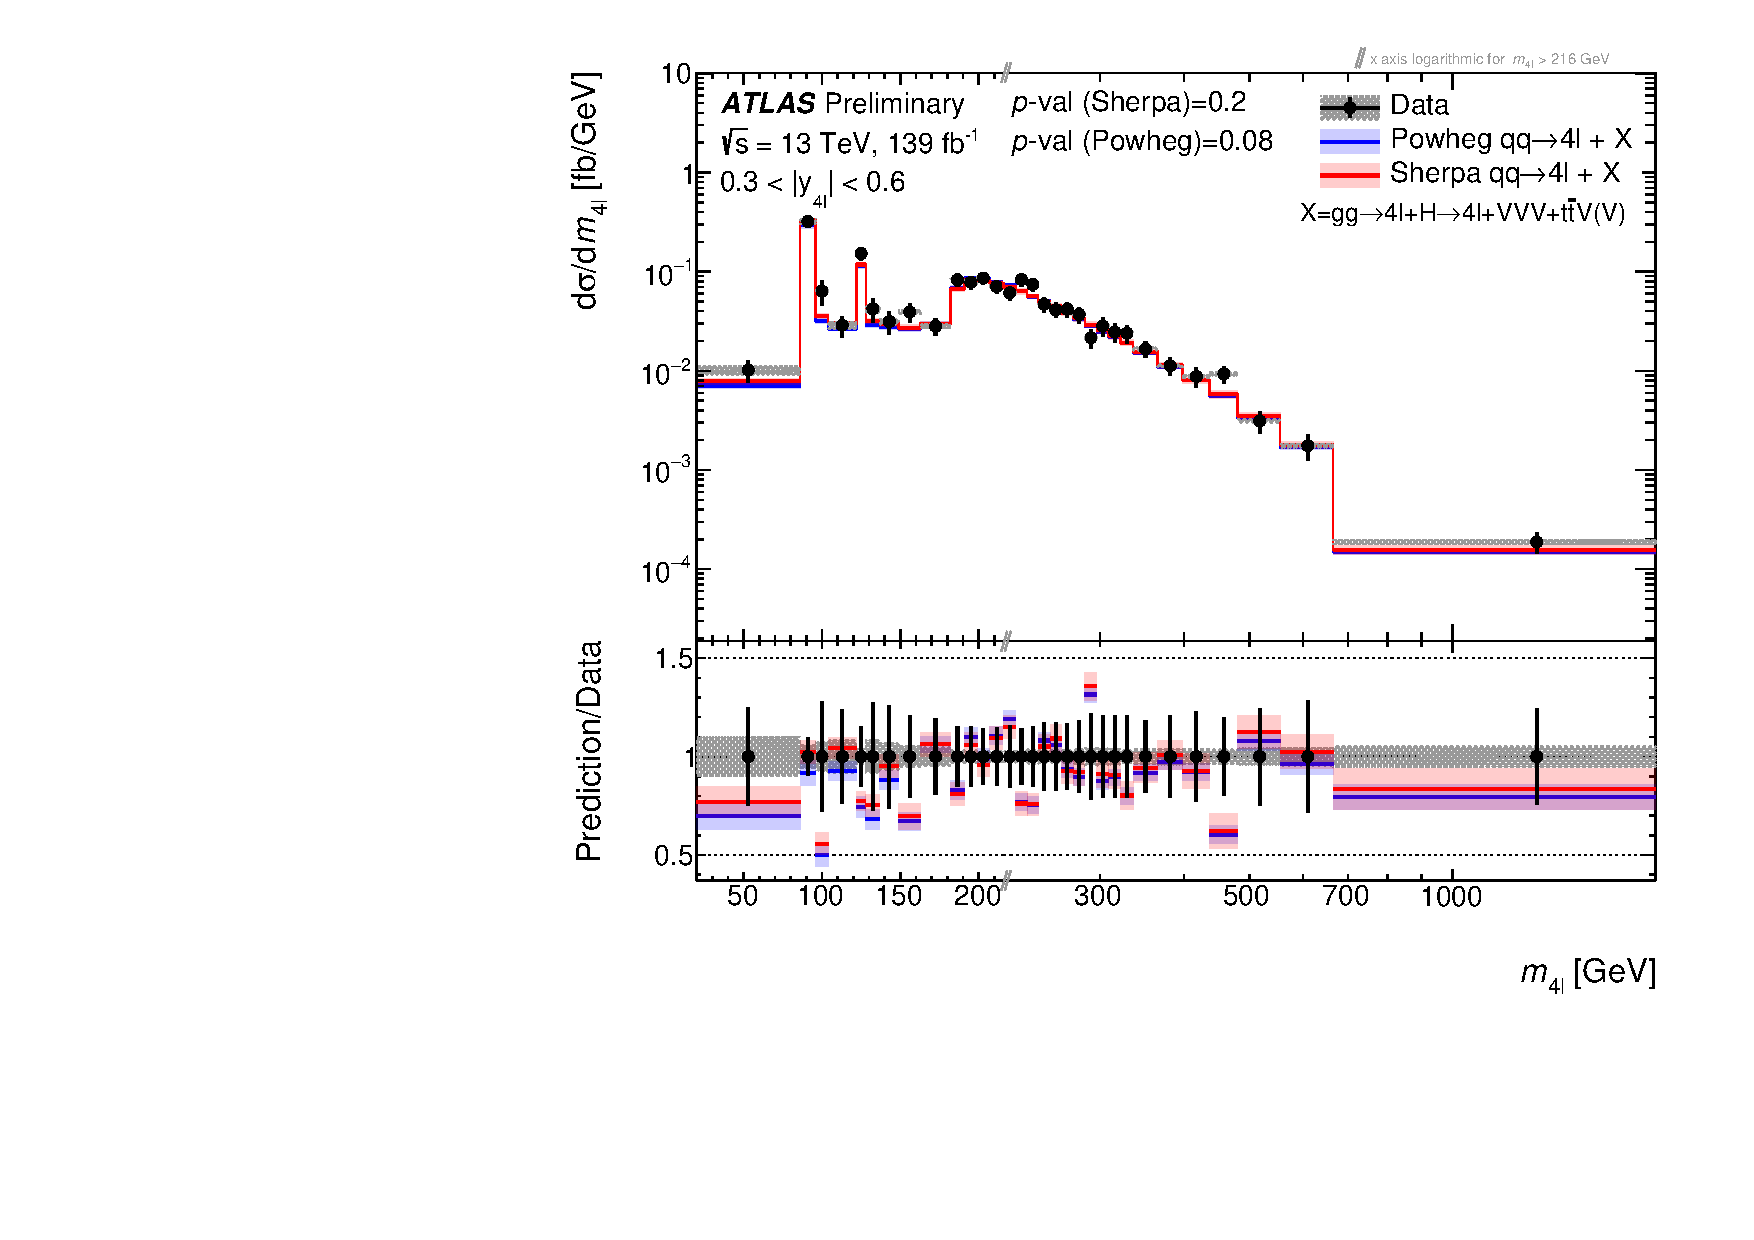
\includegraphics[width=.95\linewidth]{Figures/m4l/UnfoldedResults/linlog_Unfolded_Data_m4l_y4l0dot3-0dot6.pdf} \caption{0.3 < \yFourL{} < 0.6}\label{fig:sub-second}
    \end{subfigure}
    \begin{subfigure}{.46\textwidth}\centering
      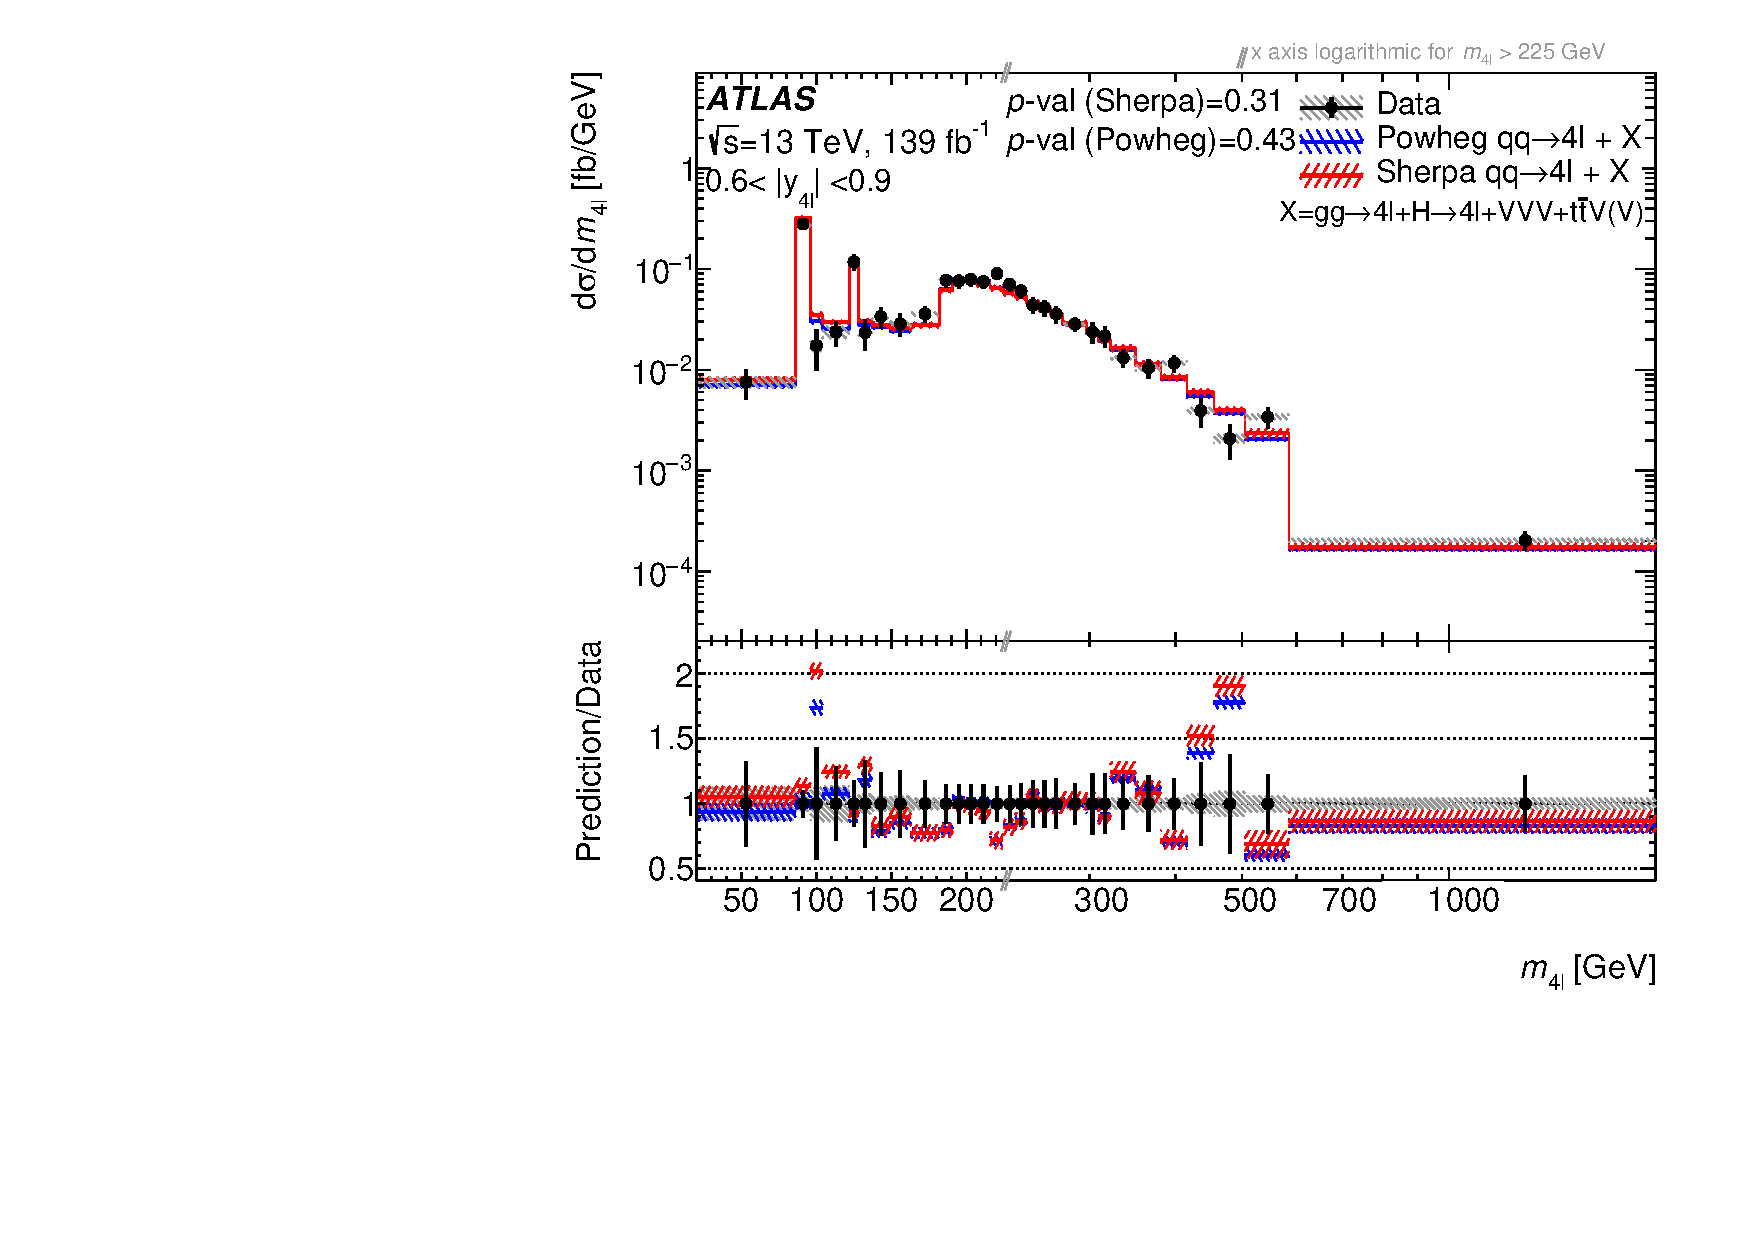
\includegraphics[width=.95\linewidth]{Figures/m4l/UnfoldedResults/linlog_Unfolded_Data_m4l_y4l0dot6-0dot9.pdf}  \caption{0.6 < \yFourL{} < 0.9}\label{fig:sub-third}
    \end{subfigure}
    \begin{subfigure}{.46\textwidth}\centering
      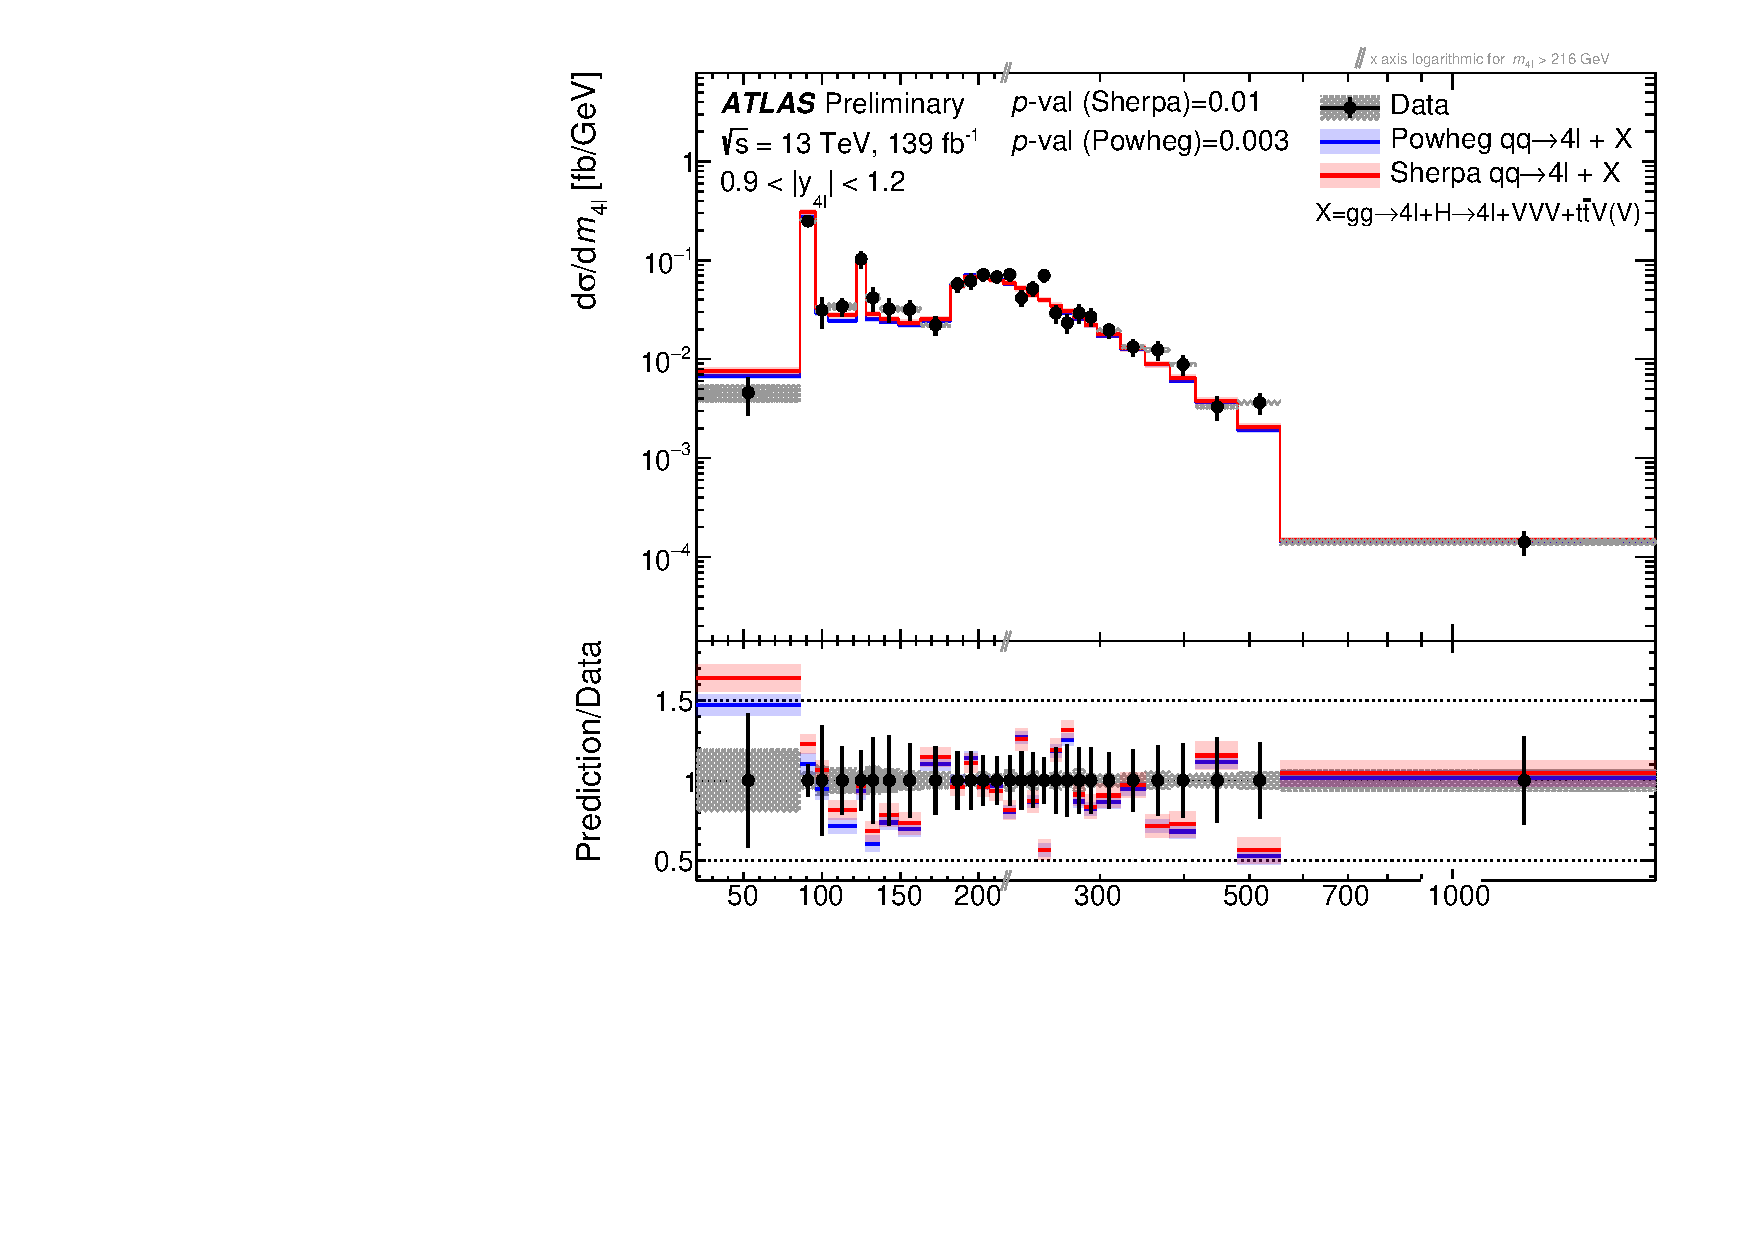
\includegraphics[width=.95\linewidth]{Figures/m4l/UnfoldedResults/linlog_Unfolded_Data_m4l_y4l0dot9-1dot2.pdf}  \caption{0.9 < \yFourL{} < 1.2}\label{fig:sub-fourth}
    \end{subfigure}
        \begin{subfigure}{.46\textwidth}\centering
      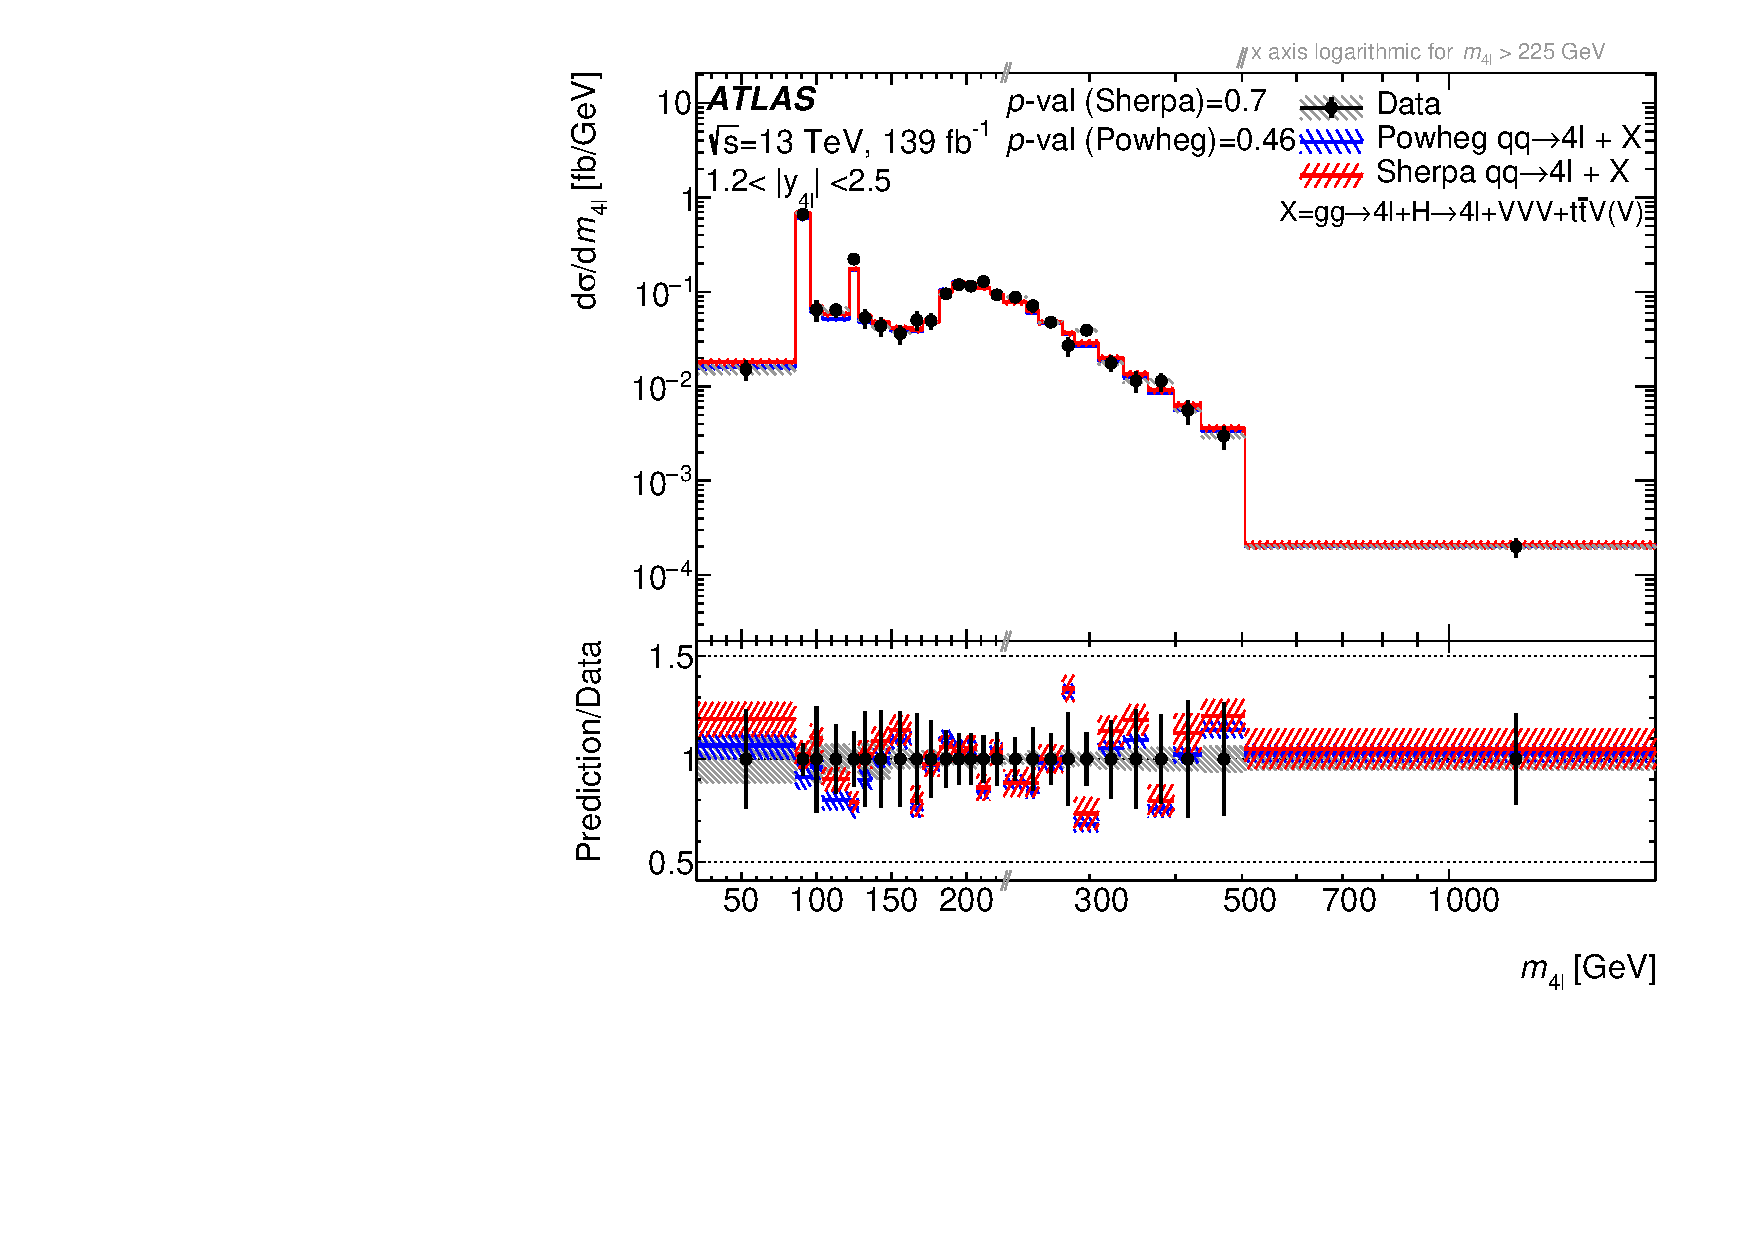
\includegraphics[width=.95\linewidth]{Figures/m4l/UnfoldedResults/linlog_Unfolded_Data_m4l_y4l1dot2-2dot5.pdf}  \caption{1.2 < \yFourL{} < 2.5}\label{fig:sub-fifth}
    \end{subfigure}
    \caption{Differential cross-section as a function of \mFourL{} in slices of \yFourL{}. \errorbars{} \SMpredictions{} \Pvalue{} The ratio of the \SHERPA{} prediction to the data is shown in the lower panel.}
    \label{fig:m4l_y4l}
\end{figure}

%% m4l vs flavour
\begin{figure}[H]
    \begin{subfigure}{.49\textwidth}\centering
      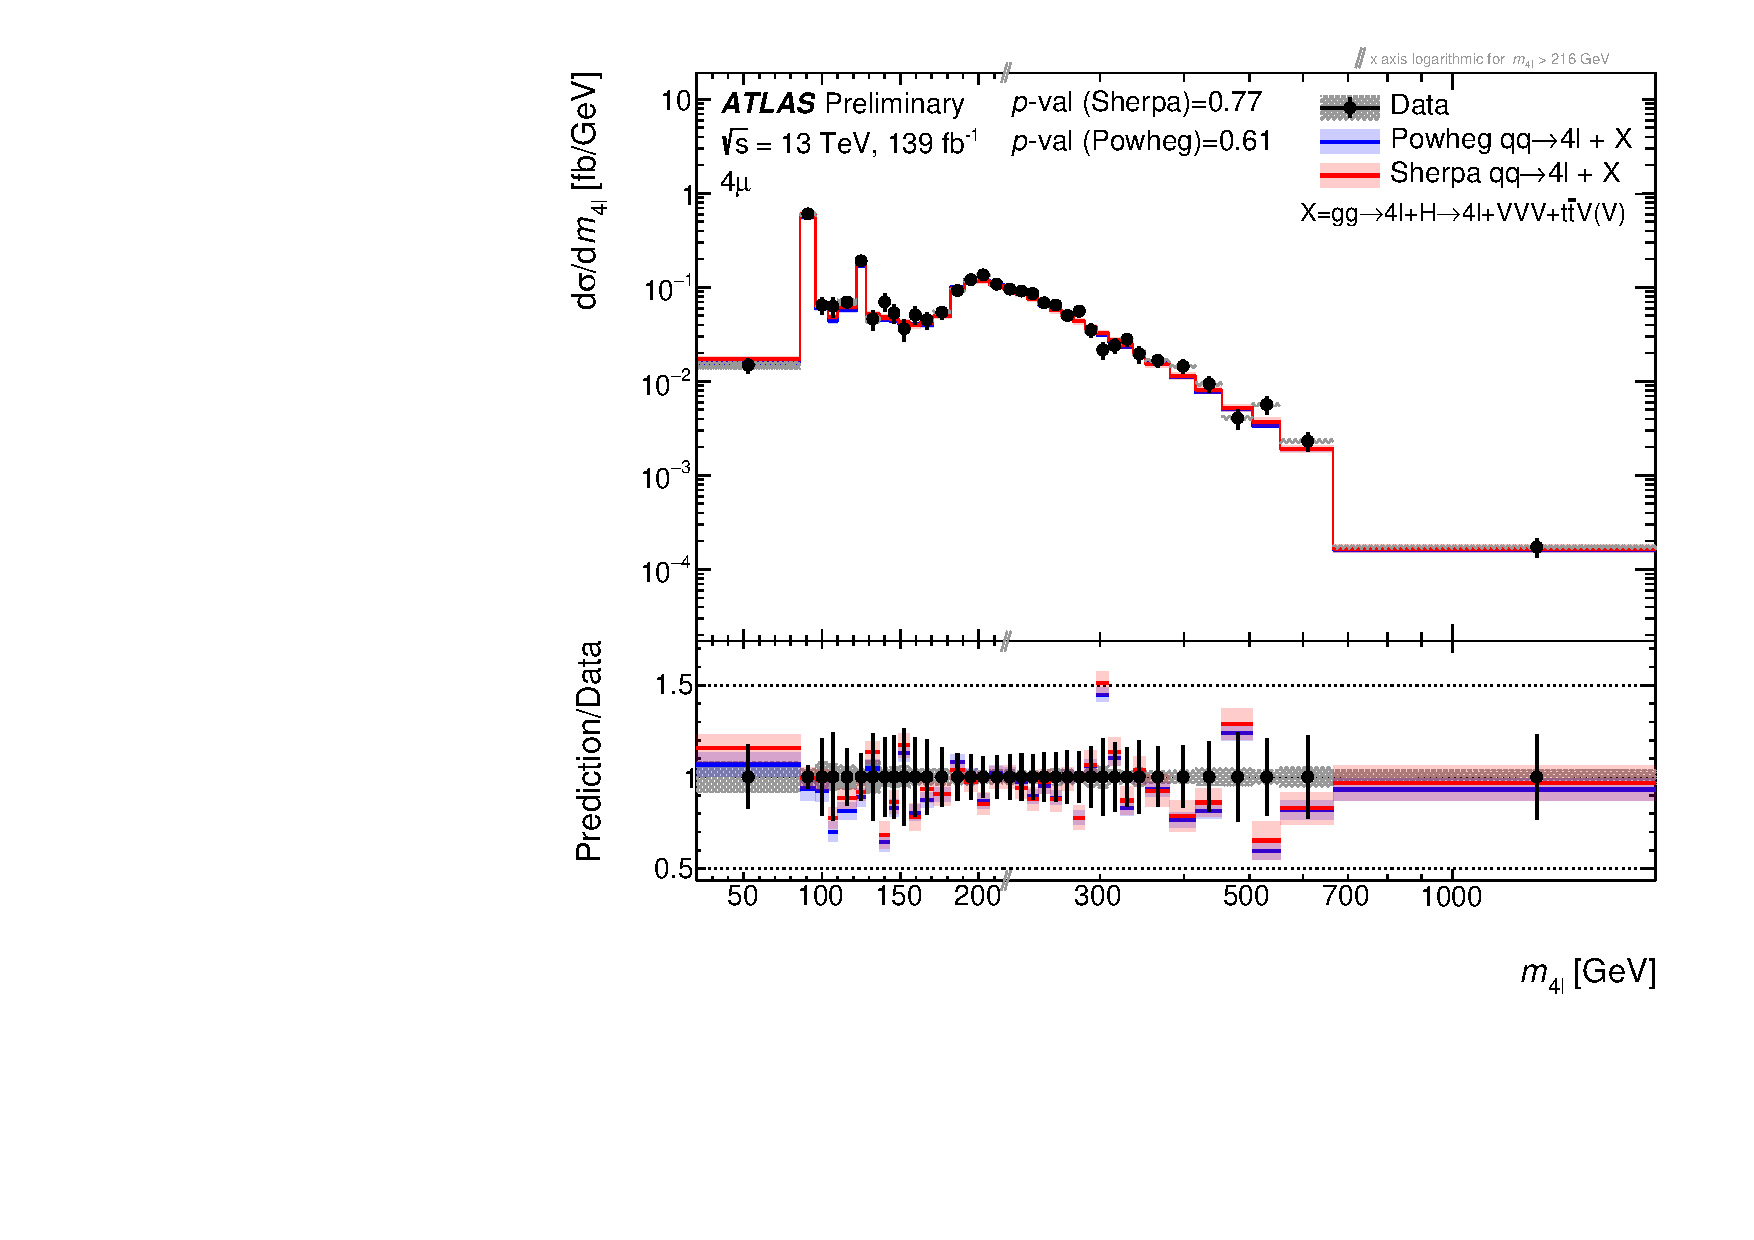
\includegraphics[width=.95\linewidth]{Figures/m4l/UnfoldedResults/linlog_Unfolded_Data_m4l_event_type4mu.pdf}\caption{$4\mu$ channel}\label{fig:sub-first}
    \end{subfigure}
    \begin{subfigure}{.49\textwidth}\centering
      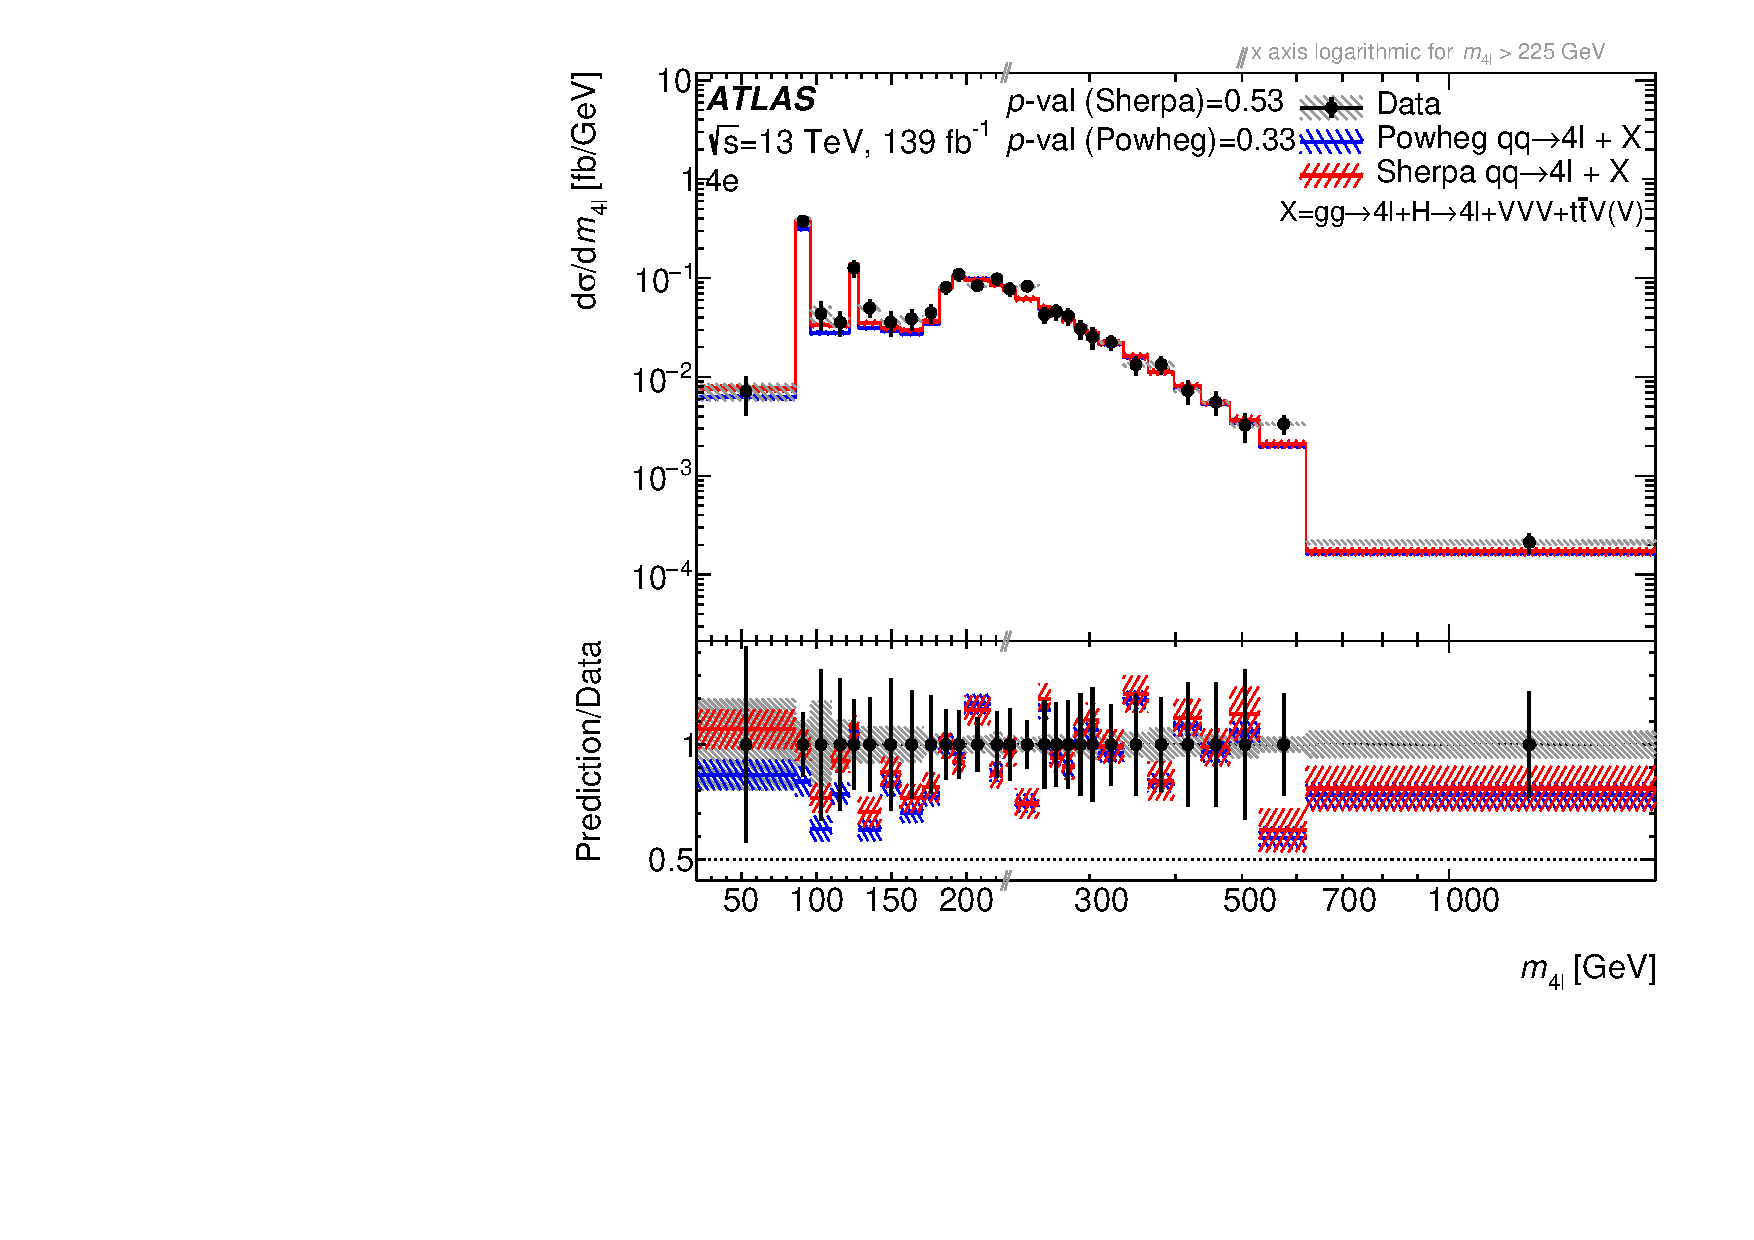
\includegraphics[width=.95\linewidth]{Figures/m4l/UnfoldedResults/linlog_Unfolded_Data_m4l_event_type4e.pdf} \caption{$4e$ channel}\label{fig:sub-second}
    \end{subfigure}
    \begin{subfigure}{.49\textwidth}\centering
      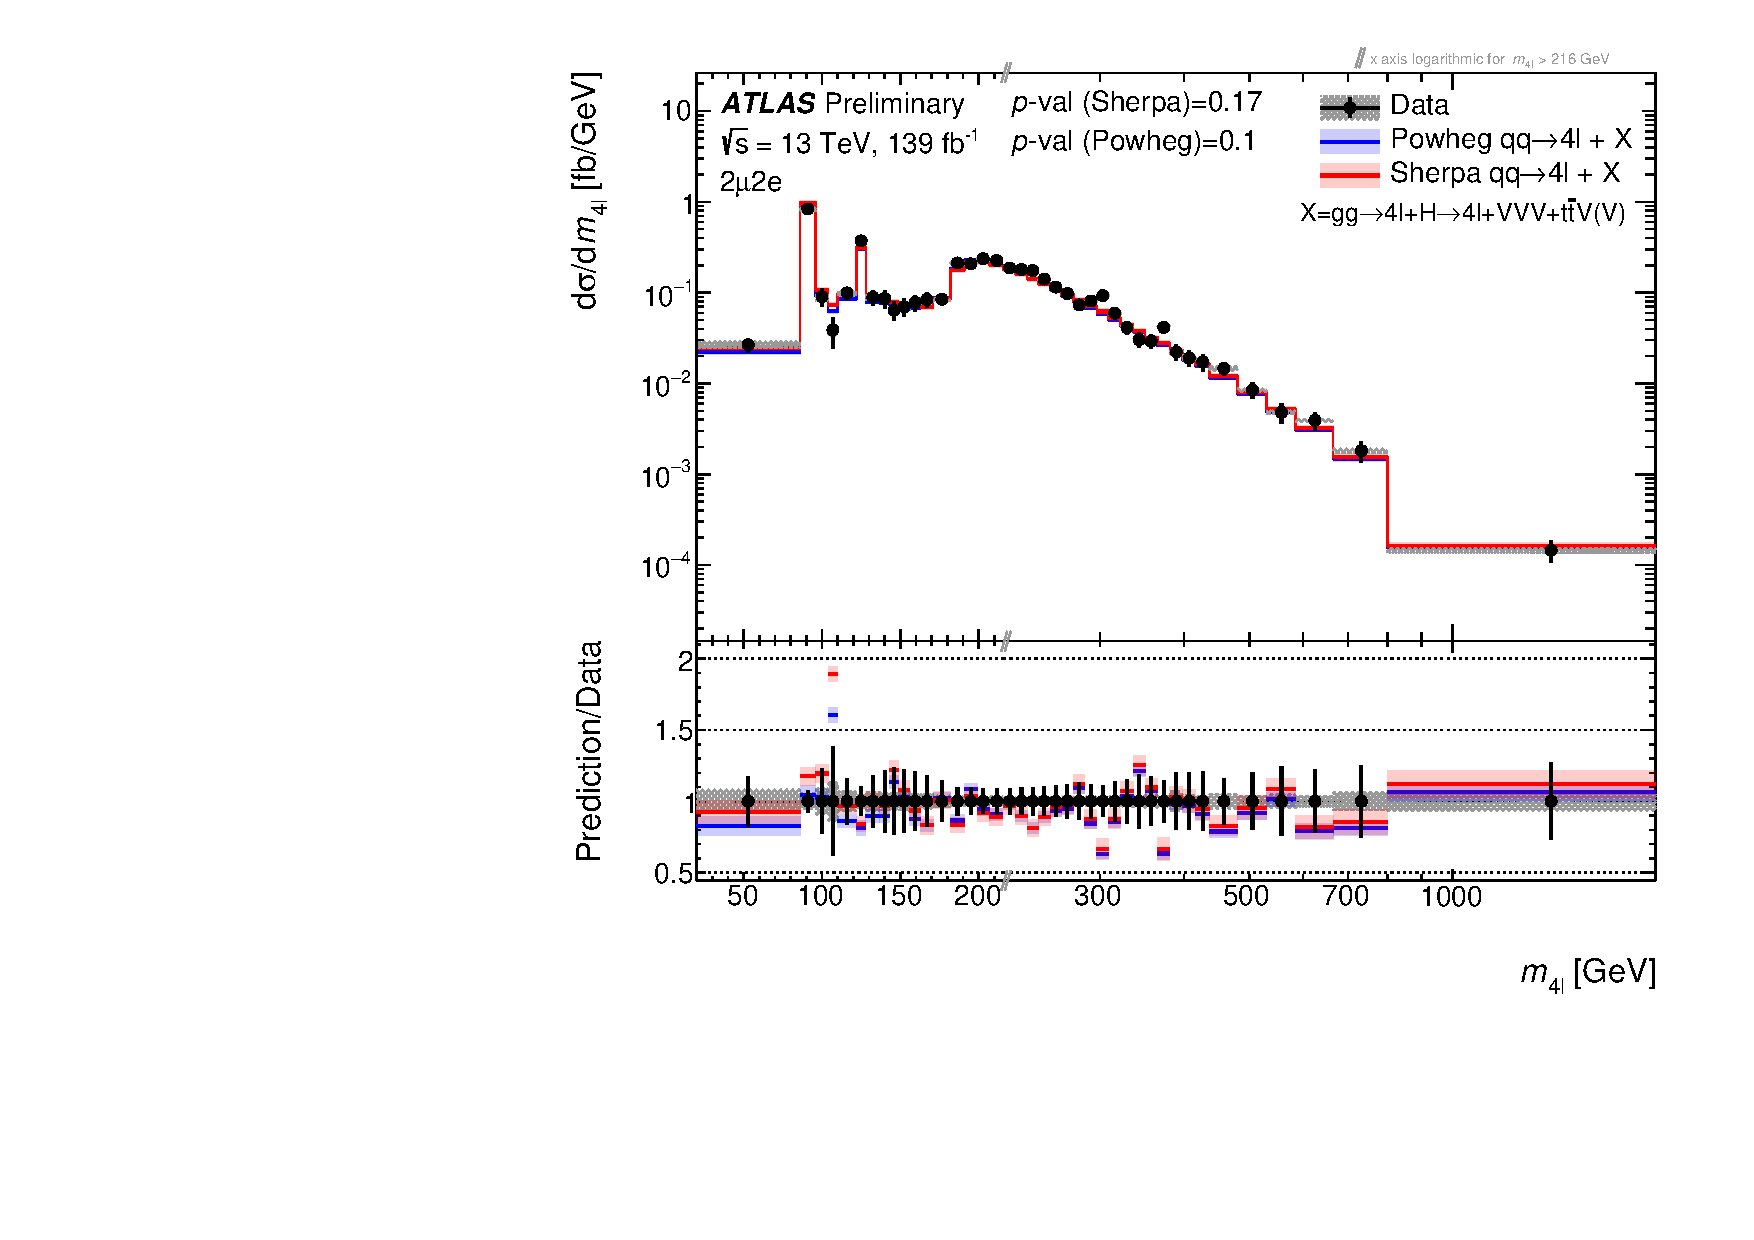
\includegraphics[width=.95\linewidth]{Figures/m4l/UnfoldedResults/linlog_Unfolded_Data_m4l_event_type2mu2e.pdf}  \caption{$2e2\mu$ channel}\label{fig:sub-third}
    \end{subfigure}
    \caption{Differential cross-section as a function of \mFourL{} for each lepton flavour channel. \errorbars{} \SMpredictions{} \Pvalue{} The ratio of the \SHERPA{} prediction to the data is shown in the lower panel. The $x$-axis is on a linear scale until $\mFourL = 225$~\GeV, where it switches to a logarithmic scale.}
    \label{fig:m4l_flavour}
\end{figure}

%% m12 vs m4l
\begin{figure}[H]
    \begin{subfigure}{.49\textwidth}\centering
      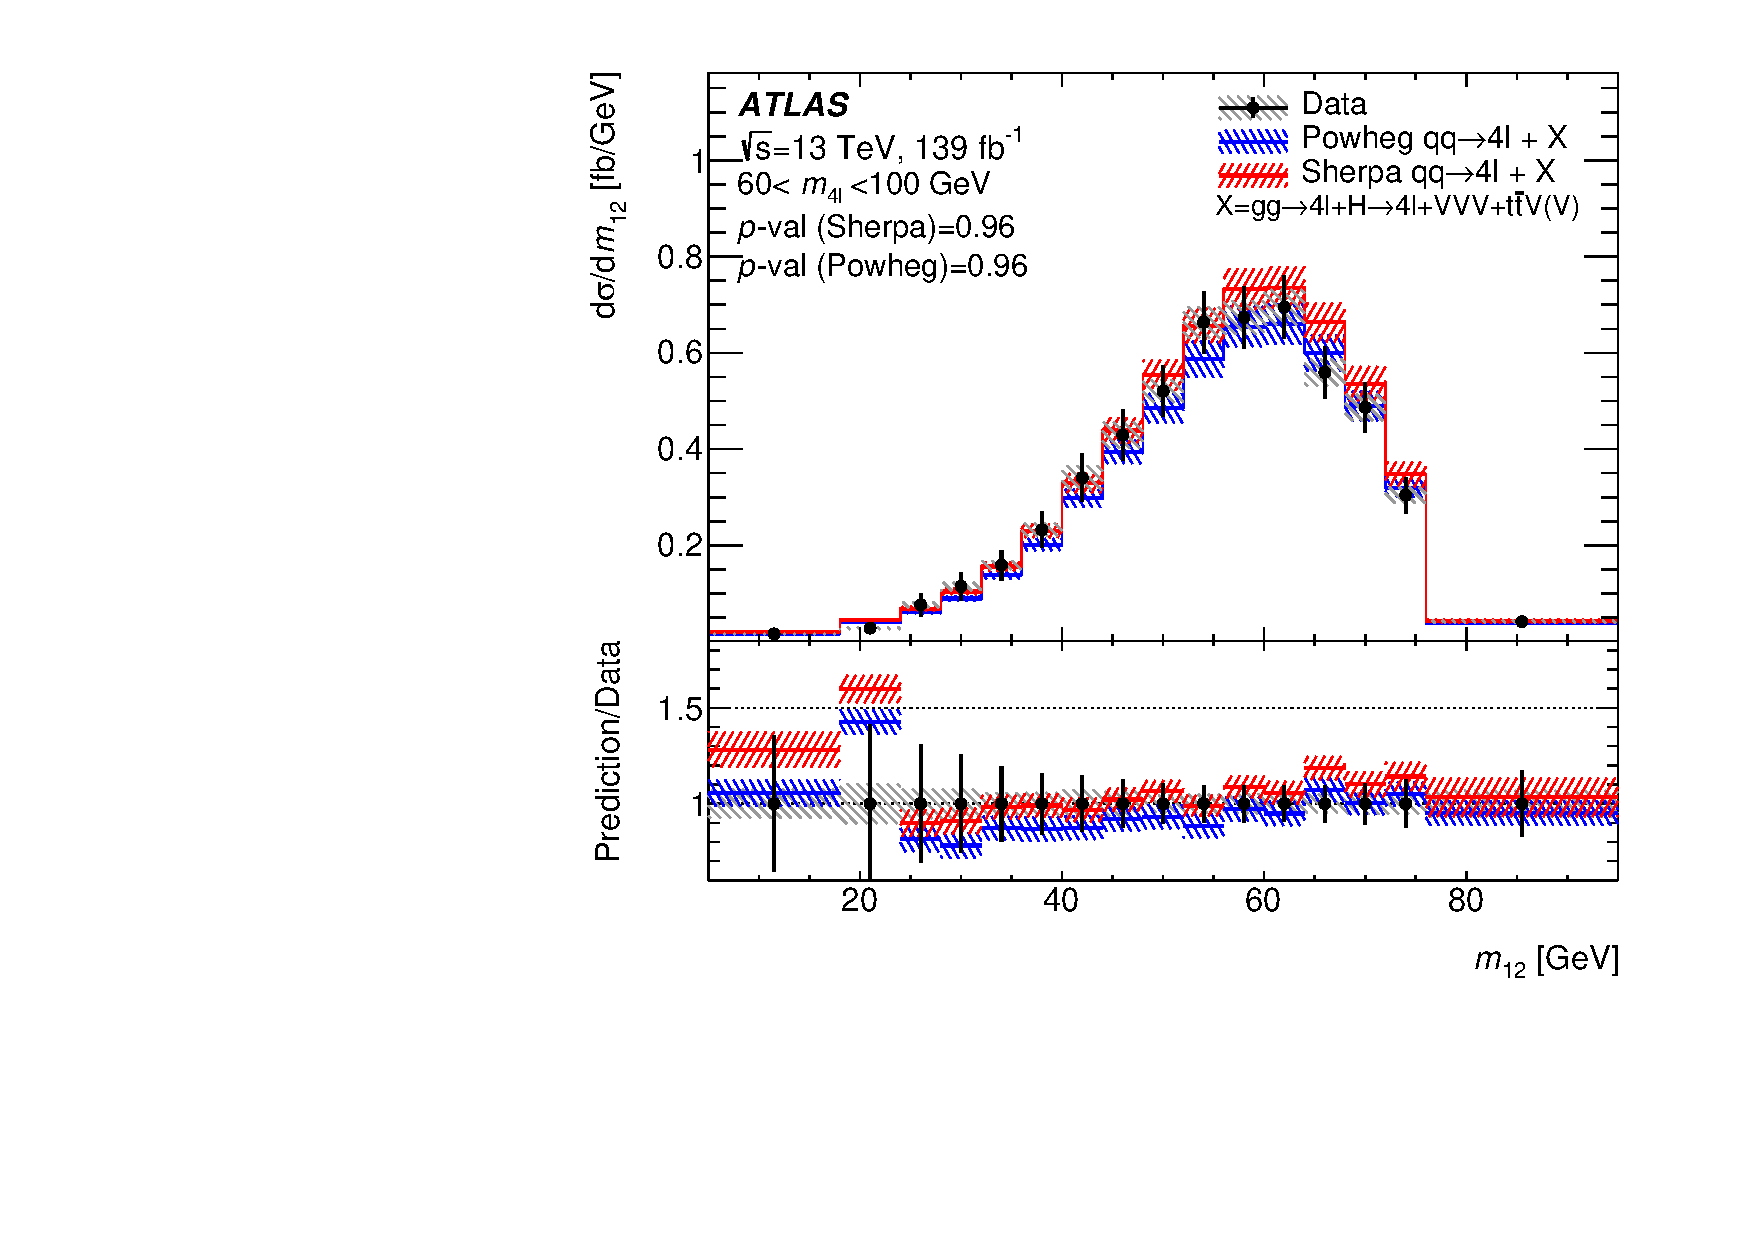
\includegraphics[width=.95\linewidth]{Figures/m4l/UnfoldedResults/linY_Unfolded_Data_m12_m4l60-100.pdf}  
      \caption{\ZFourL \ region}
      \label{fig:sub-first}
    \end{subfigure}
    \begin{subfigure}{.49\textwidth}\centering
      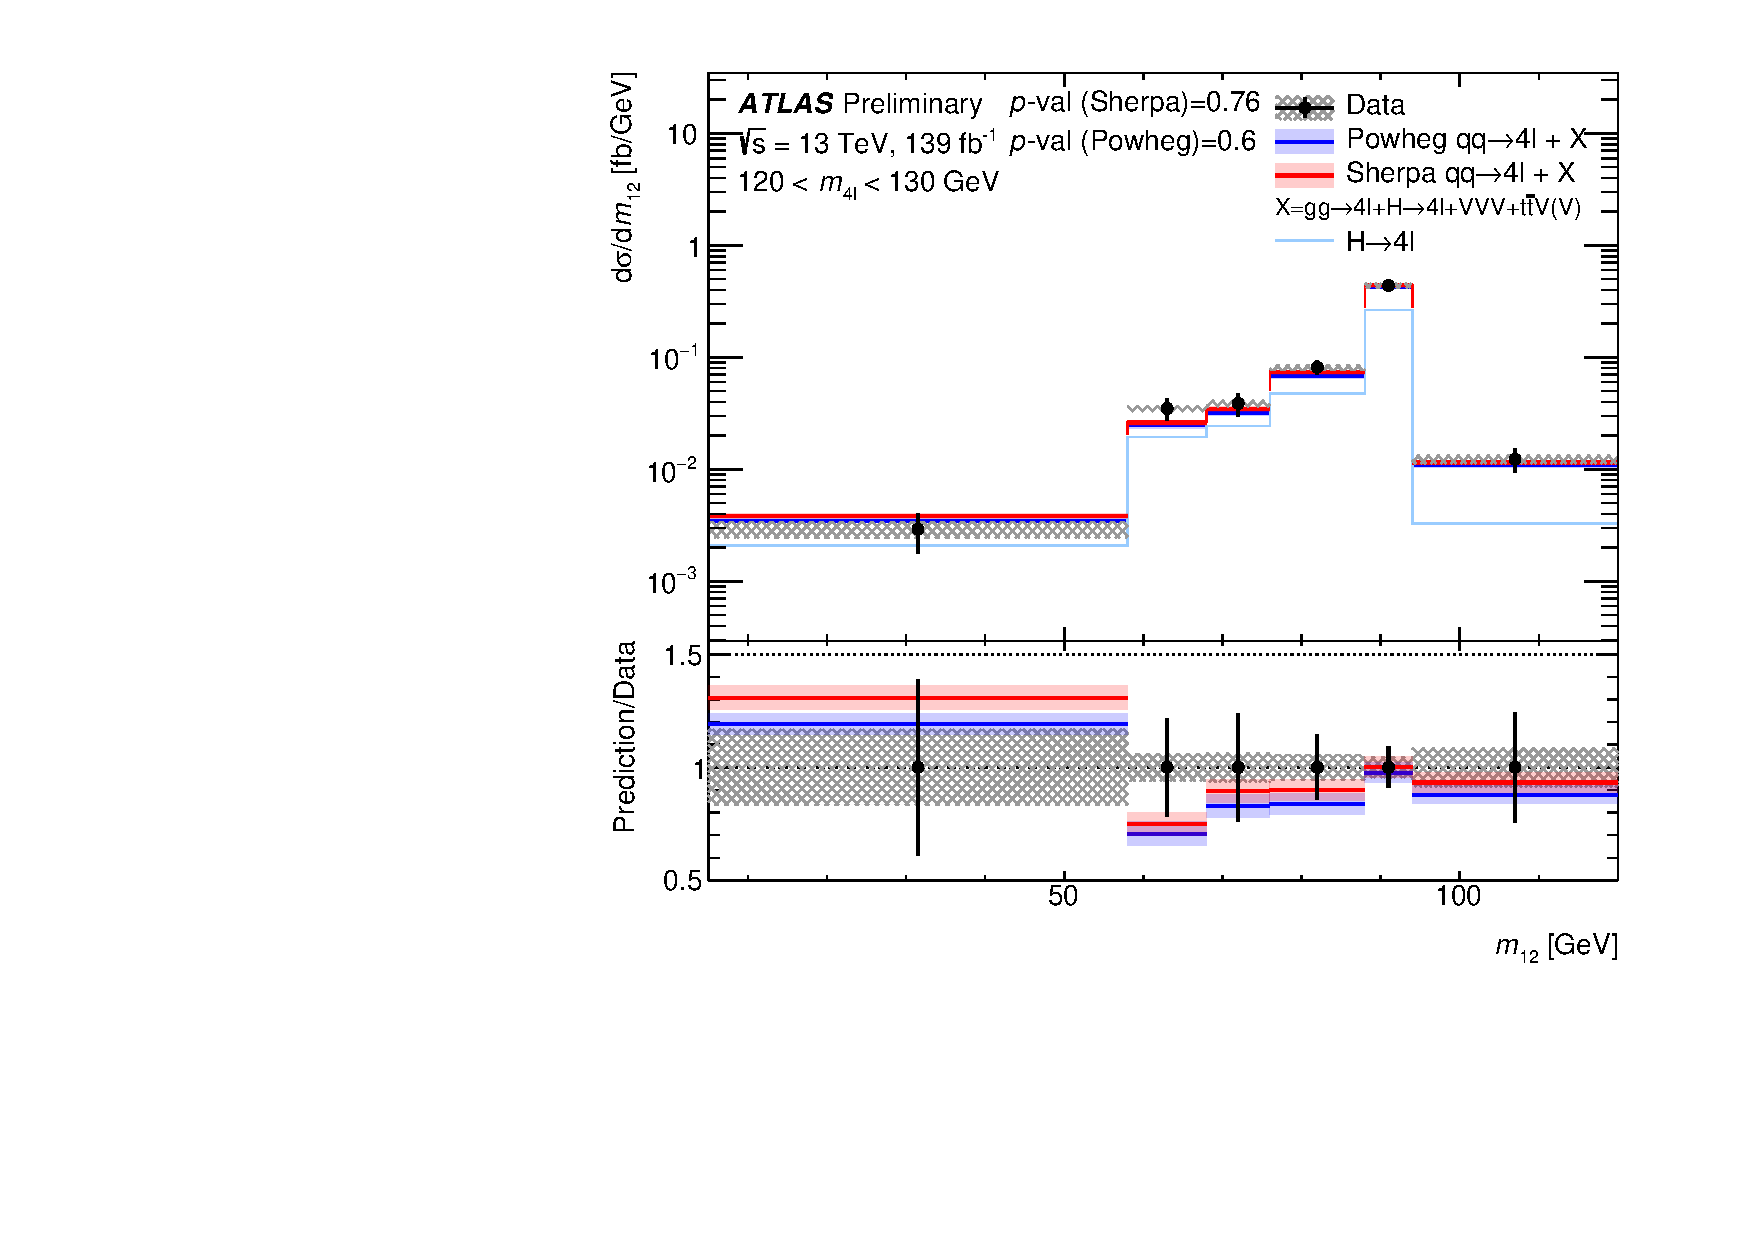
\includegraphics[width=.95\linewidth]{Figures/m4l/UnfoldedResults/higgs_Unfolded_Data_m12_m4l120-130.pdf}  
      \caption{\HFourL \ region}
      \label{fig:sub-second}
    \end{subfigure}
    \begin{subfigure}{.49\textwidth}
      \centering
      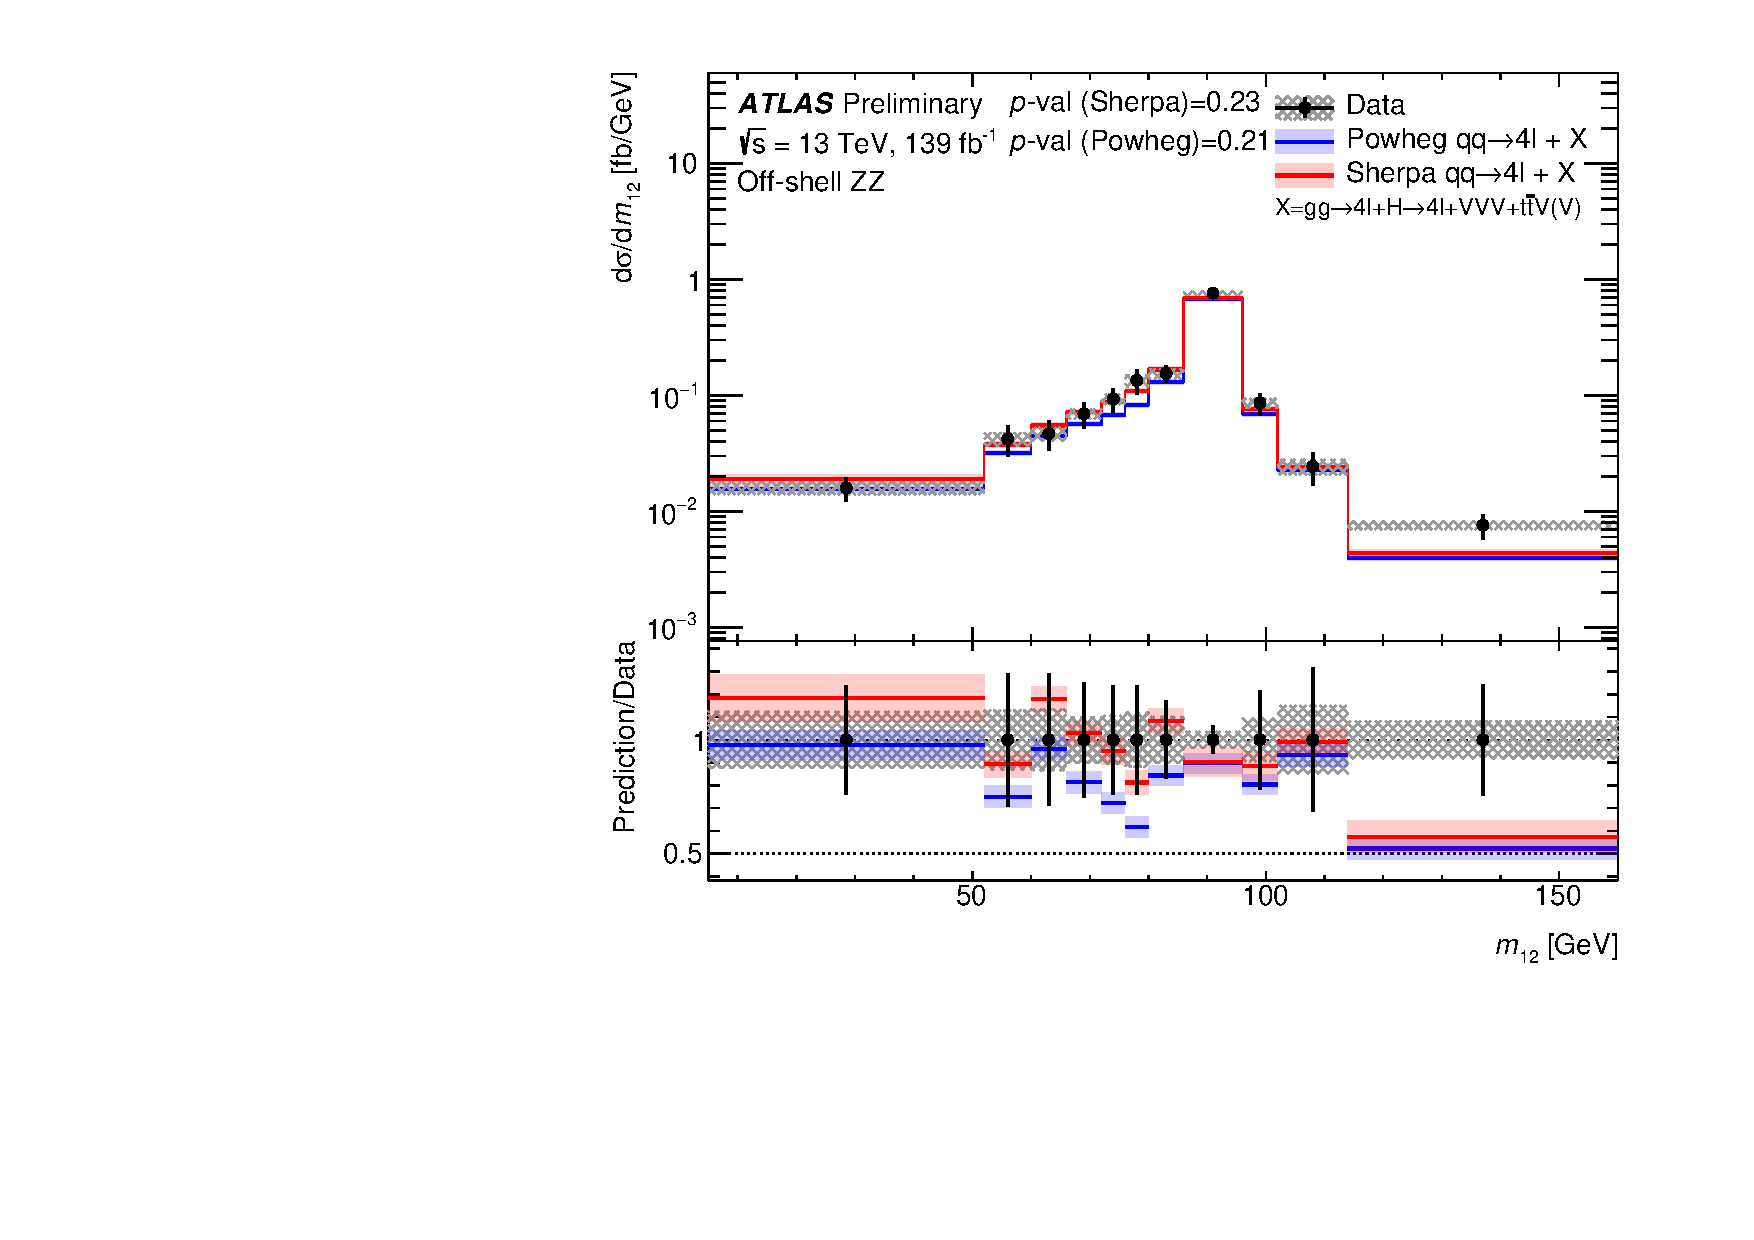
\includegraphics[width=.95\linewidth]{Figures/m4l/UnfoldedResults/Unfolded_Data_m12_m4loffshell.pdf}  
      \caption{Off-shell $\Z\Z$ region}
      \label{fig:sub-third}
    \end{subfigure}
    \begin{subfigure}{.49\textwidth}
      \centering
      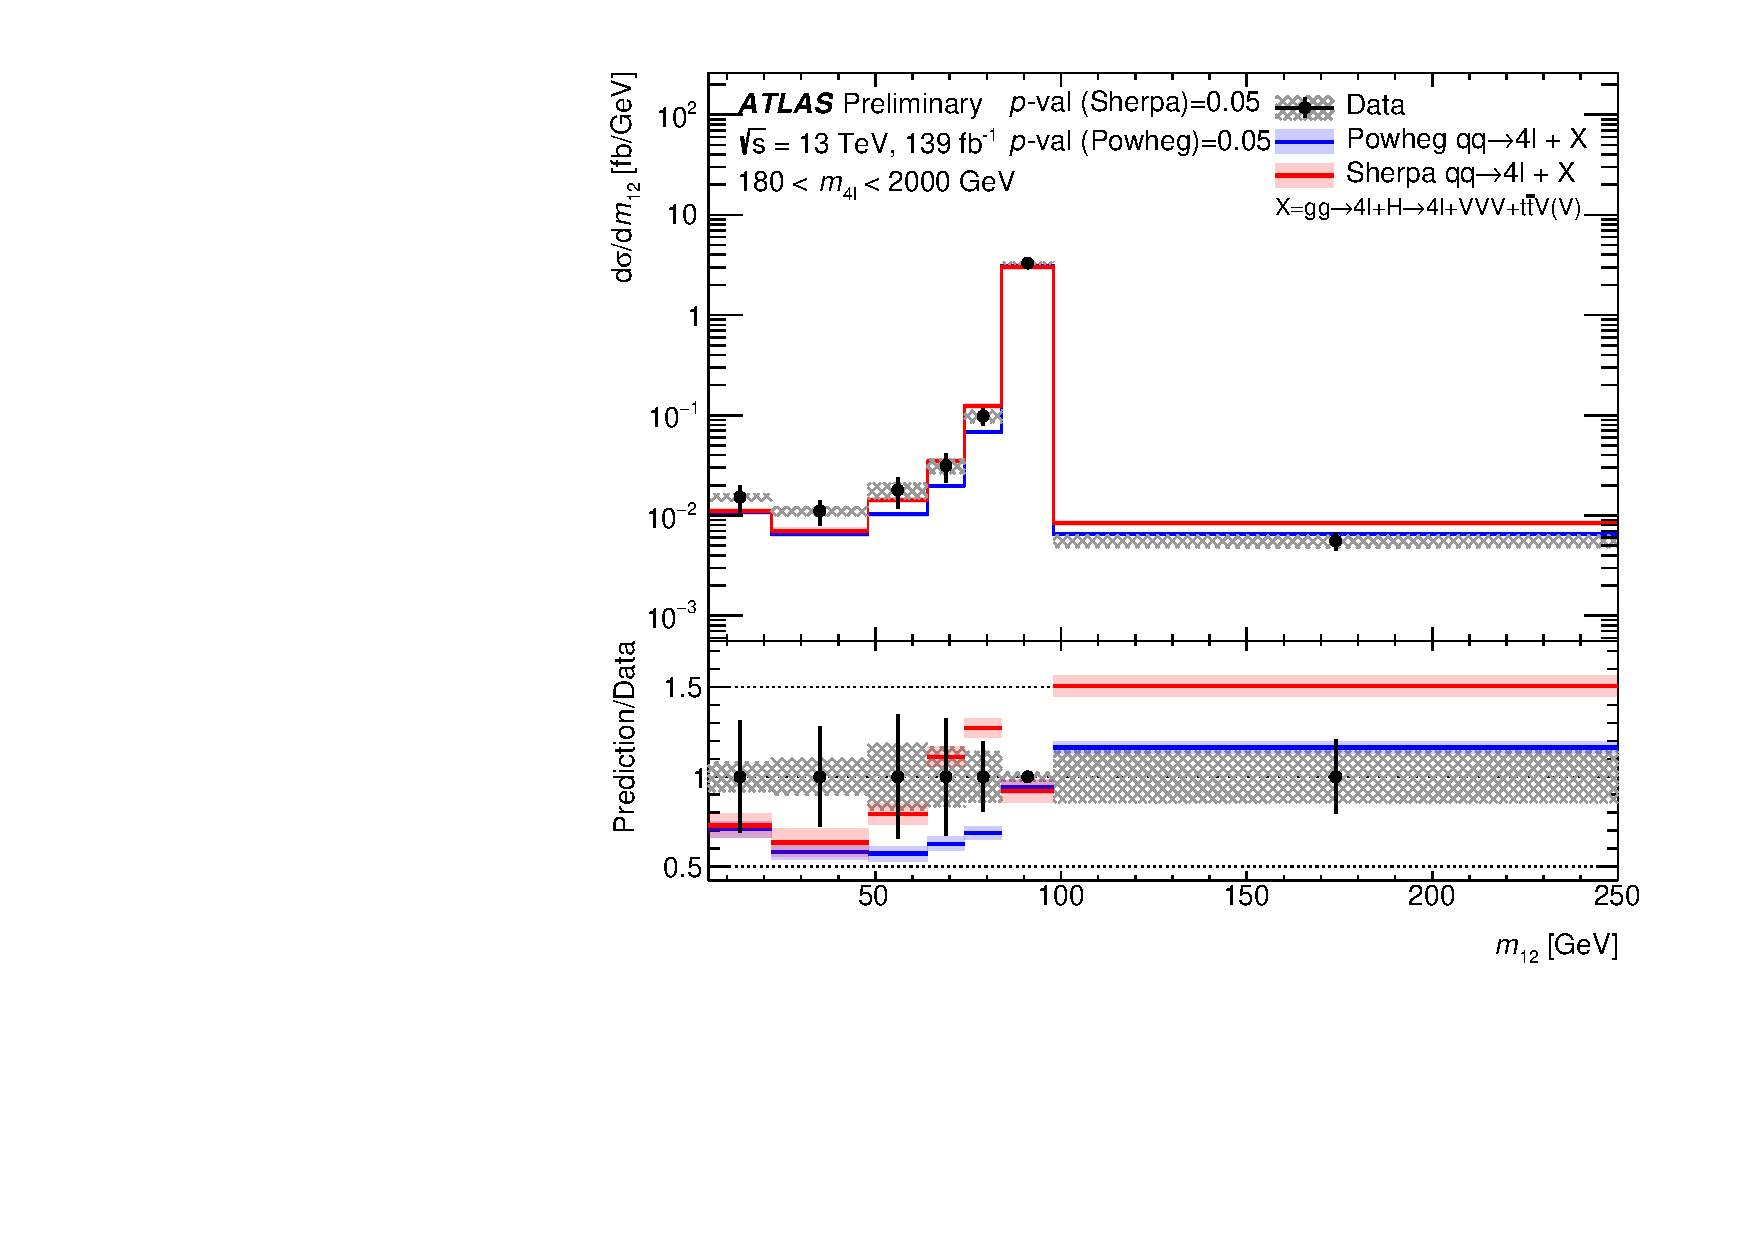
\includegraphics[width=.95\linewidth]{Figures/m4l/UnfoldedResults/Unfolded_Data_m12_m4l180-2000.pdf}  
      \caption{On-shell $\Z\Z$ region}
      \label{fig:sub-fourth}
    \end{subfigure}
    \caption{Differential cross-section as a function of \mZOne{} in the four
        \mFourL{} regions. \errorbars{} \SMpredictions{} \Pvalue{} The ratio of the \SHERPA{} prediction to the data is shown in the lower panel. In (b) the contribution from Higgs production is shown in addition to the total SM prediction.}
    \label{fig:m12_m4l}
\end{figure}
%% m34 vs m4l
\begin{figure}[H]
    \begin{subfigure}{.49\textwidth}\centering
      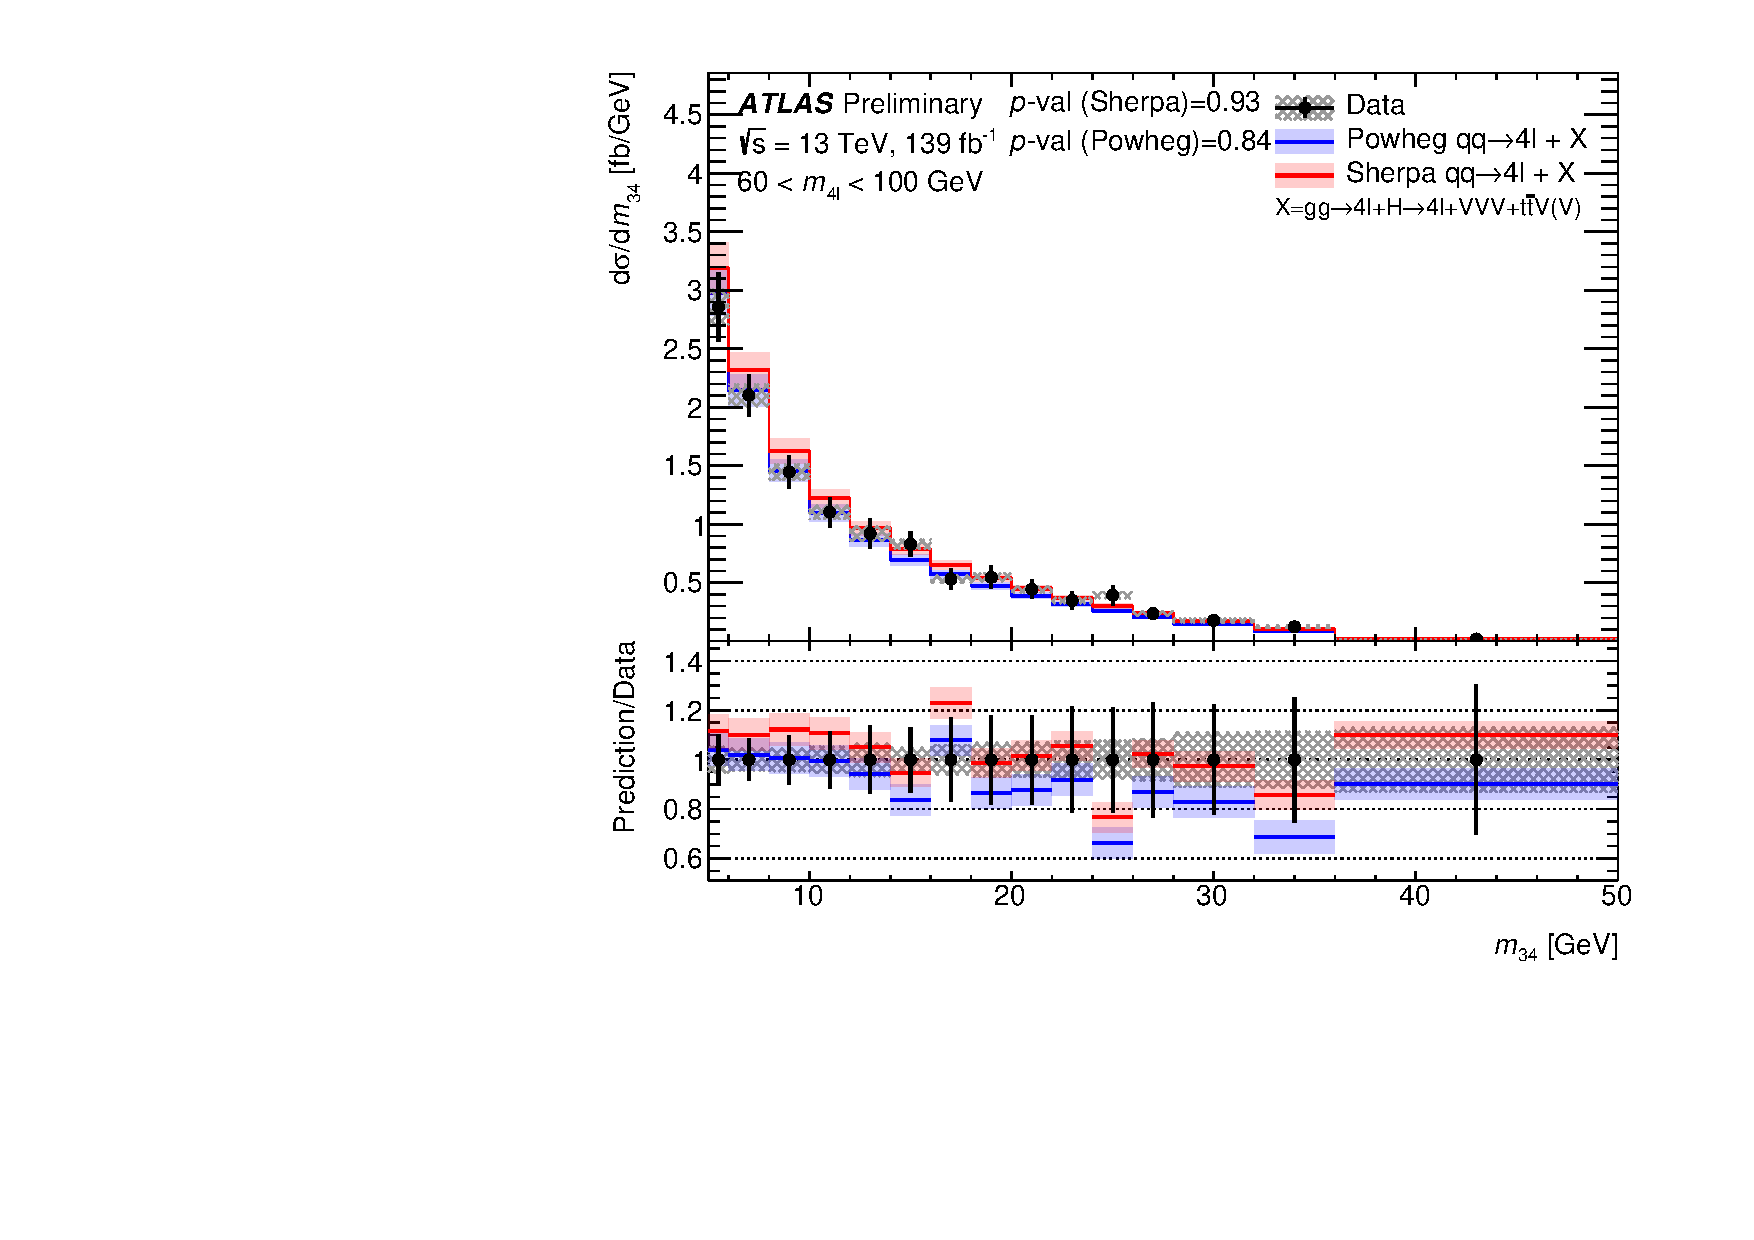
\includegraphics[width=.95\linewidth]{Figures/m4l/UnfoldedResults/linY_Unfolded_Data_m34_m4l60-100.pdf}\caption{\ZFourL \ region}\label{fig:sub-first}
    \end{subfigure}
    \begin{subfigure}{.49\textwidth}\centering
      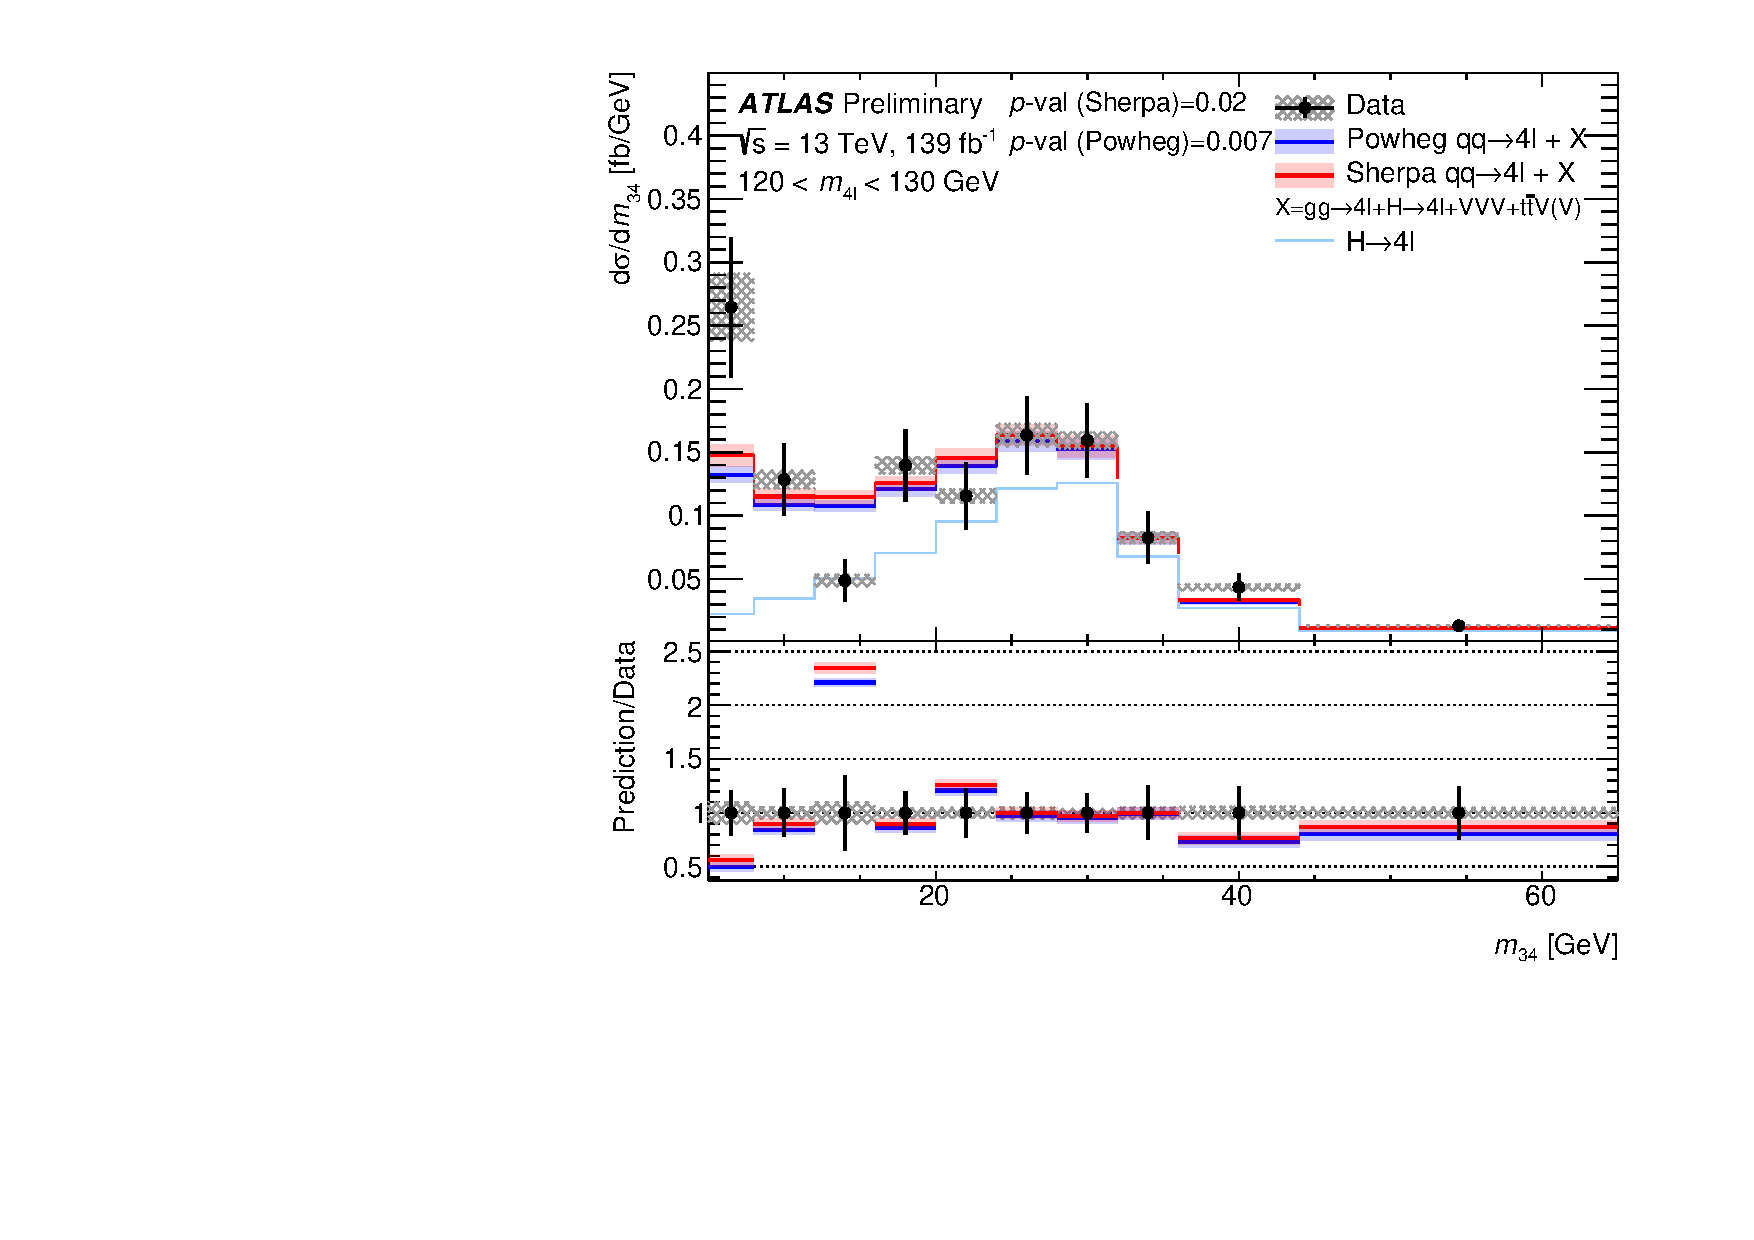
\includegraphics[width=.95\linewidth]{Figures/m4l/UnfoldedResults/higgs_linY_Unfolded_Data_m34_m4l120-130.pdf} \caption{\HFourL \ region}\label{fig:sub-second}
    \end{subfigure}
    \begin{subfigure}{.49\textwidth}\centering
      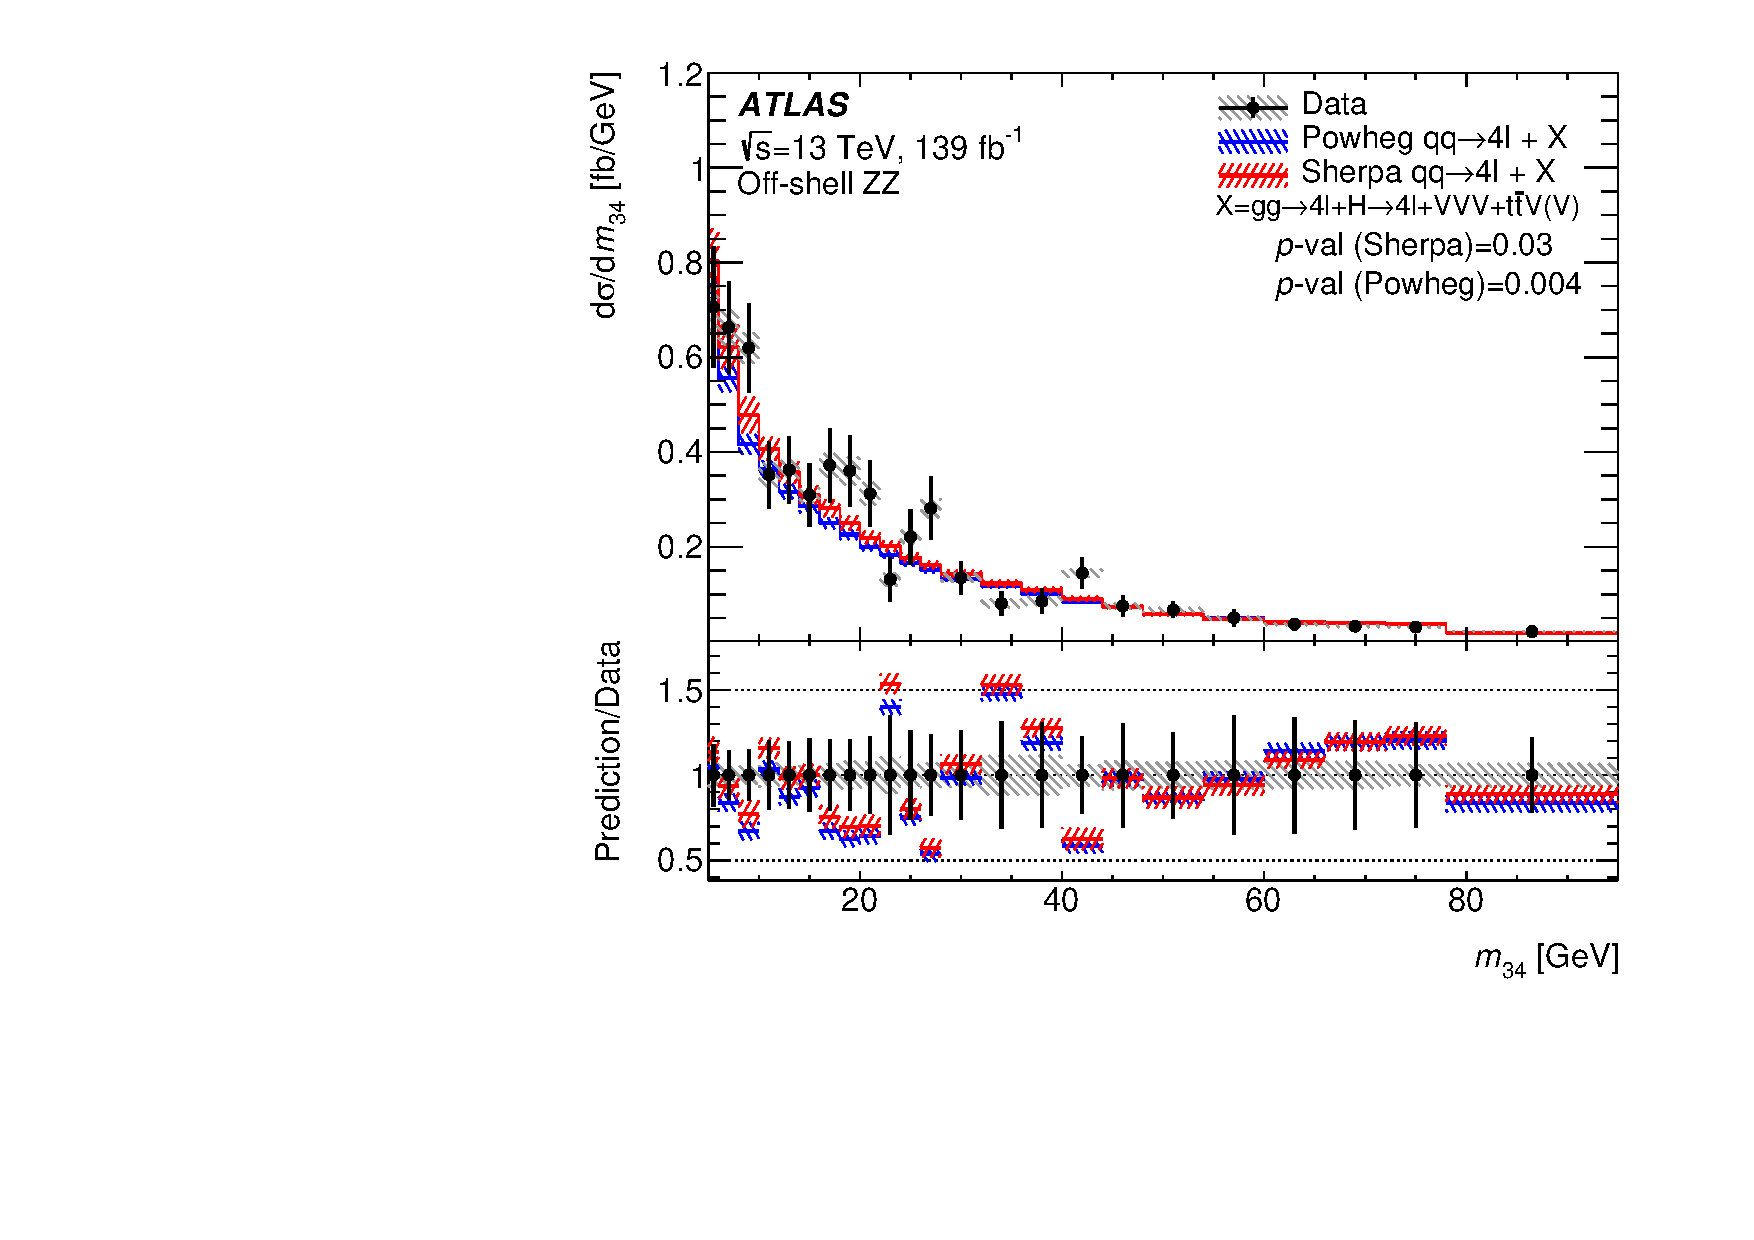
\includegraphics[width=.95\linewidth]{Figures/m4l/UnfoldedResults/linY_Unfolded_Data_m34_m4loffshell.pdf}  \caption{Off-shell $\Z\Z$ region}\label{fig:sub-third}
    \end{subfigure}
    \begin{subfigure}{.49\textwidth}\centering
      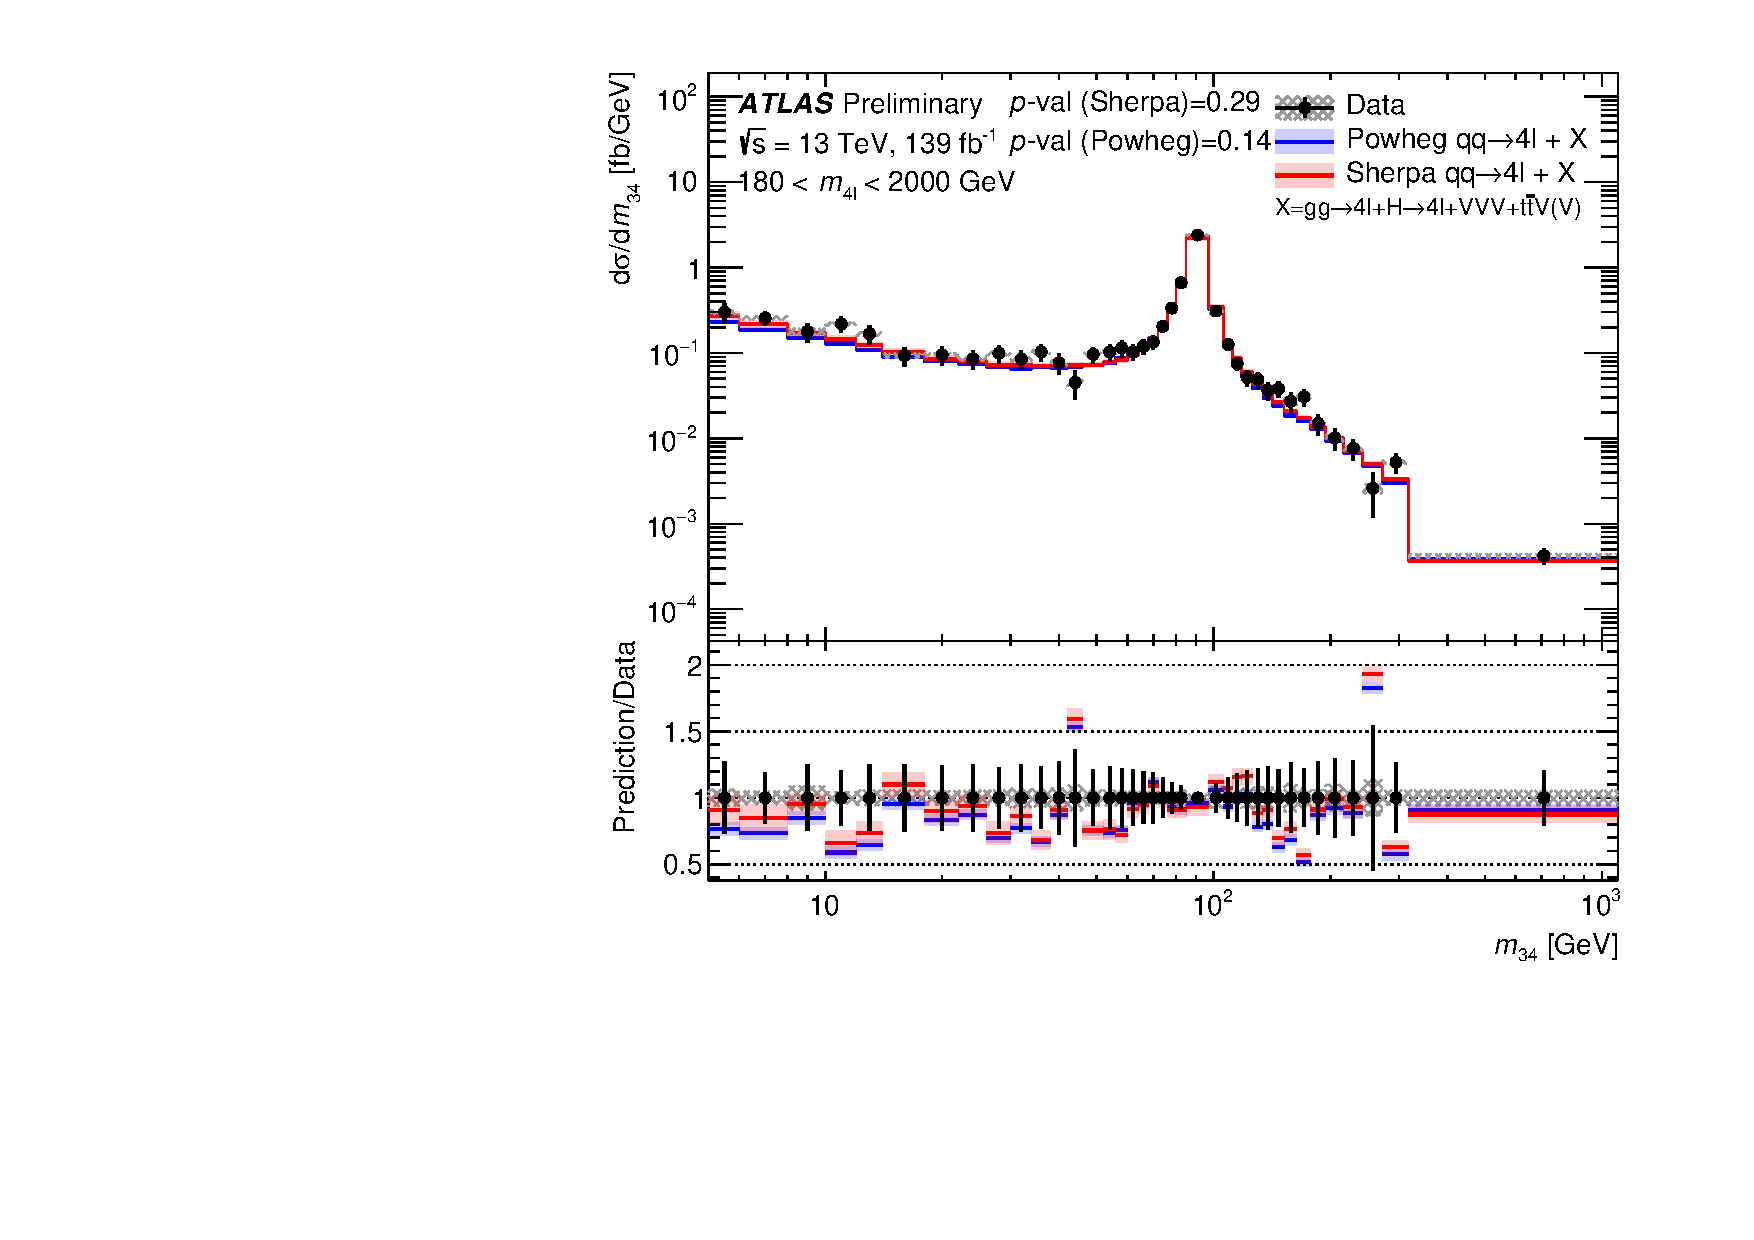
\includegraphics[width=.95\linewidth]{Figures/m4l/UnfoldedResults/Unfolded_Data_m34_m4l180-2000.pdf}  \caption{On-shell $\Z\Z$ region}\label{fig:sub-fourth}
    \end{subfigure}
    \caption{Differential cross-section as a function of \mZTwo{} in the four
        \mFourL{} regions. The measured data (black points) are  compared with the SM prediction using either \SHERPA{} (red, with red hashed band for the uncertainty) or \POWHEG{} + \pythia{} (blue, with blue hashed band for the uncertainty) to model the \qqFourL{} contribution. In (b) the contribution from Higgs production is shown in addition to the total SM prediction. The error bars on the data points give the total uncertainty and the grey hashed band gives the systematic uncertainty. \Pvalue{} The  lower panel shows the ratio of the SM predictions to the data.}
    \label{fig:m34_m4l}
\end{figure}

%% pt12 vs m4l
\begin{figure}[H]
    \begin{subfigure}{.49\textwidth}\centering
      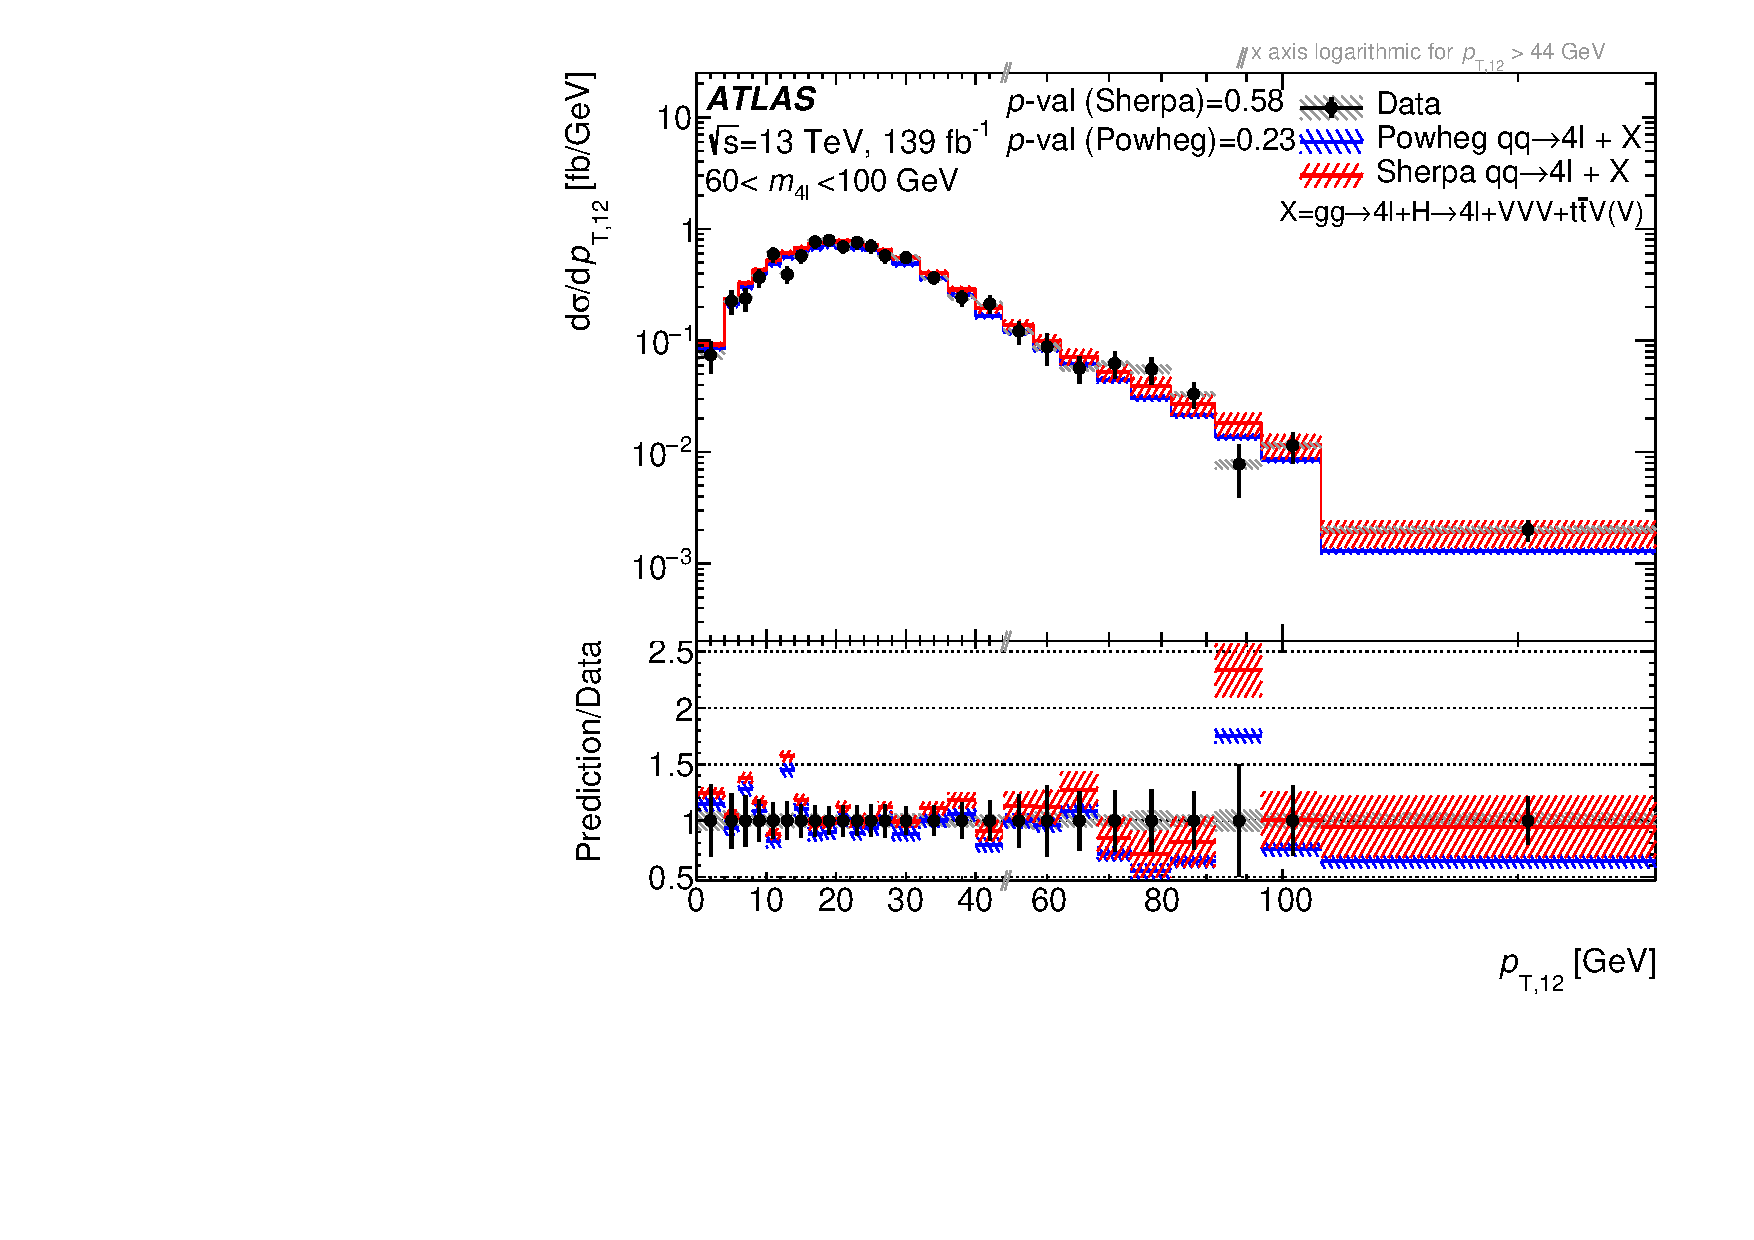
\includegraphics[width=.95\linewidth]{Figures/m4l/UnfoldedResults/linlog_Unfolded_Data_pt12_m4l60-100.pdf}\caption{\ZFourL \ region}\label{fig:sub-first}
    \end{subfigure}
    \begin{subfigure}{.49\textwidth}\centering
      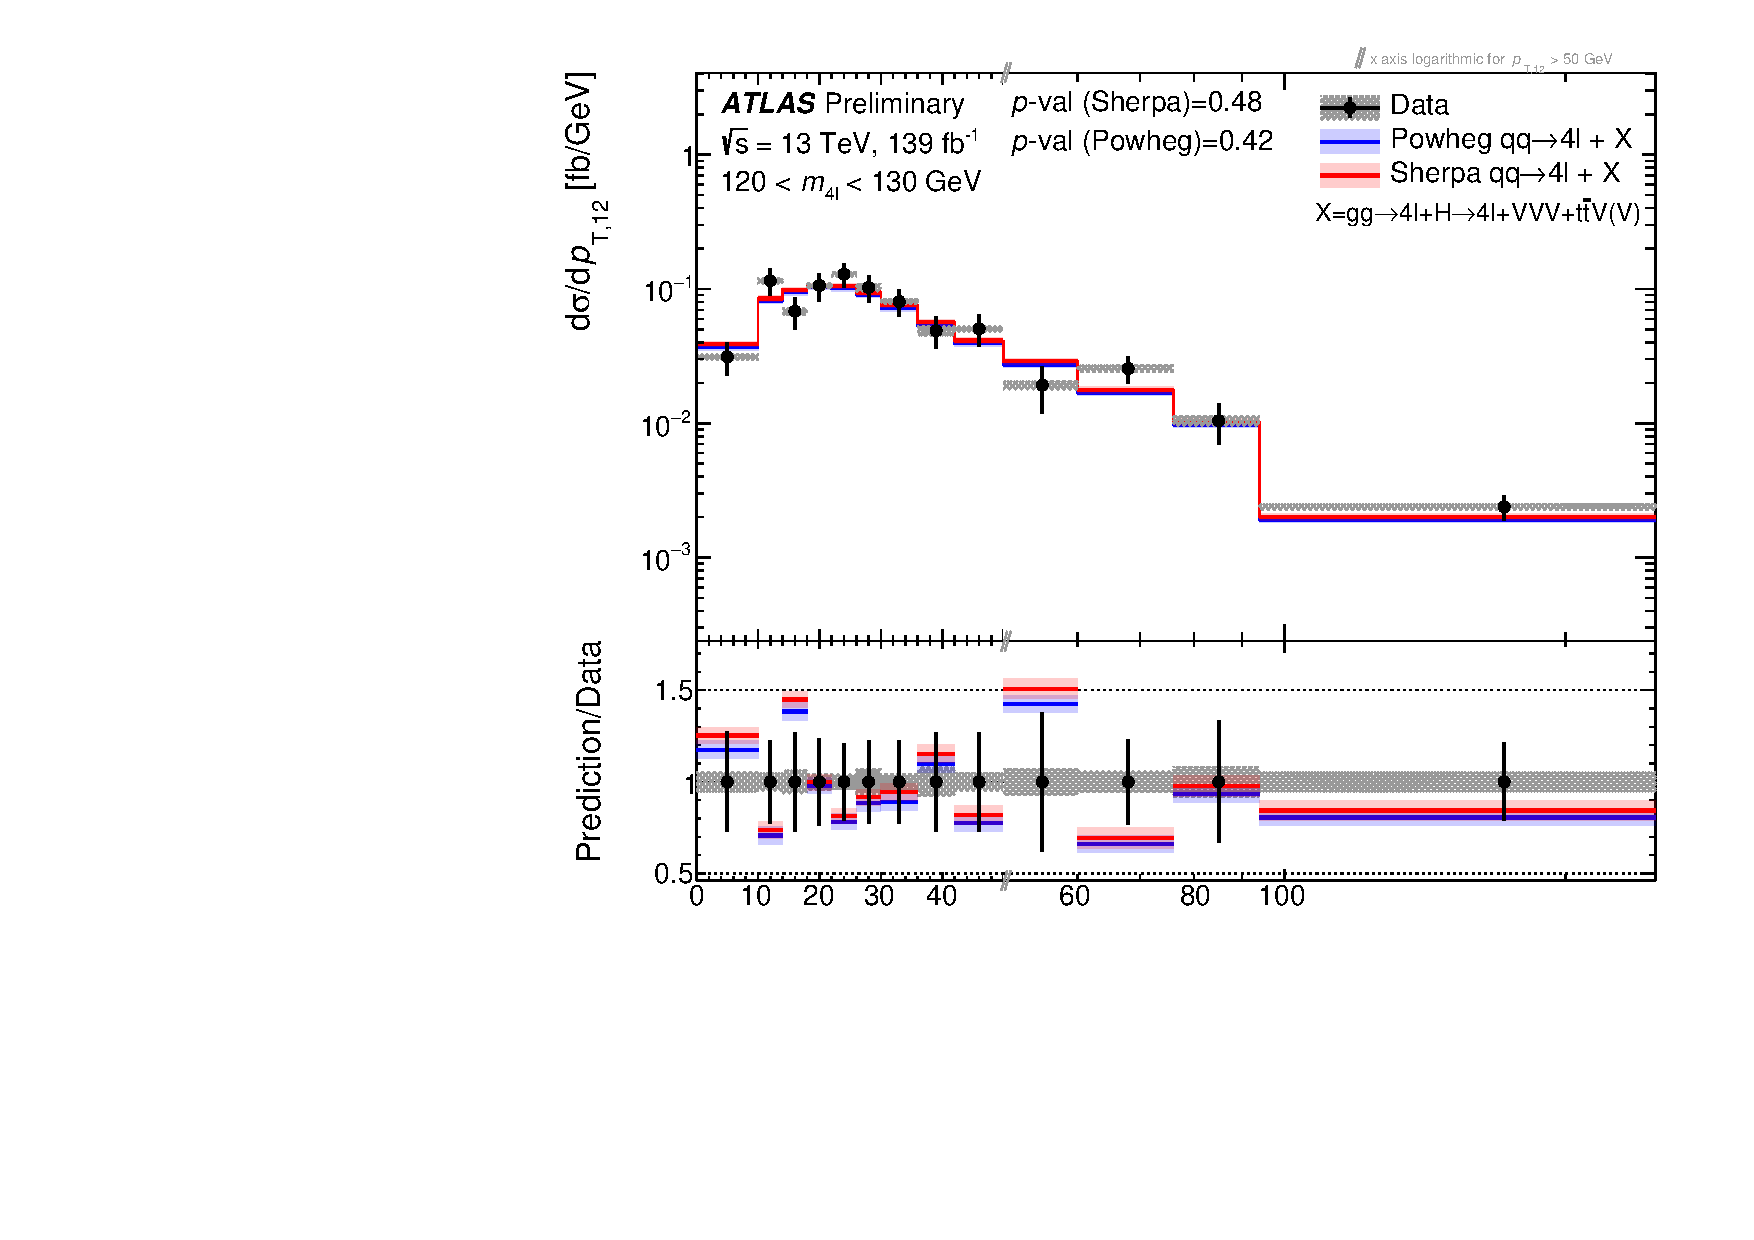
\includegraphics[width=.95\linewidth]{Figures/m4l/UnfoldedResults/linlog_Unfolded_Data_pt12_m4l120-130.pdf} \caption{\HFourL \ region}\label{fig:sub-second}
    \end{subfigure}
    \begin{subfigure}{.49\textwidth}\centering
      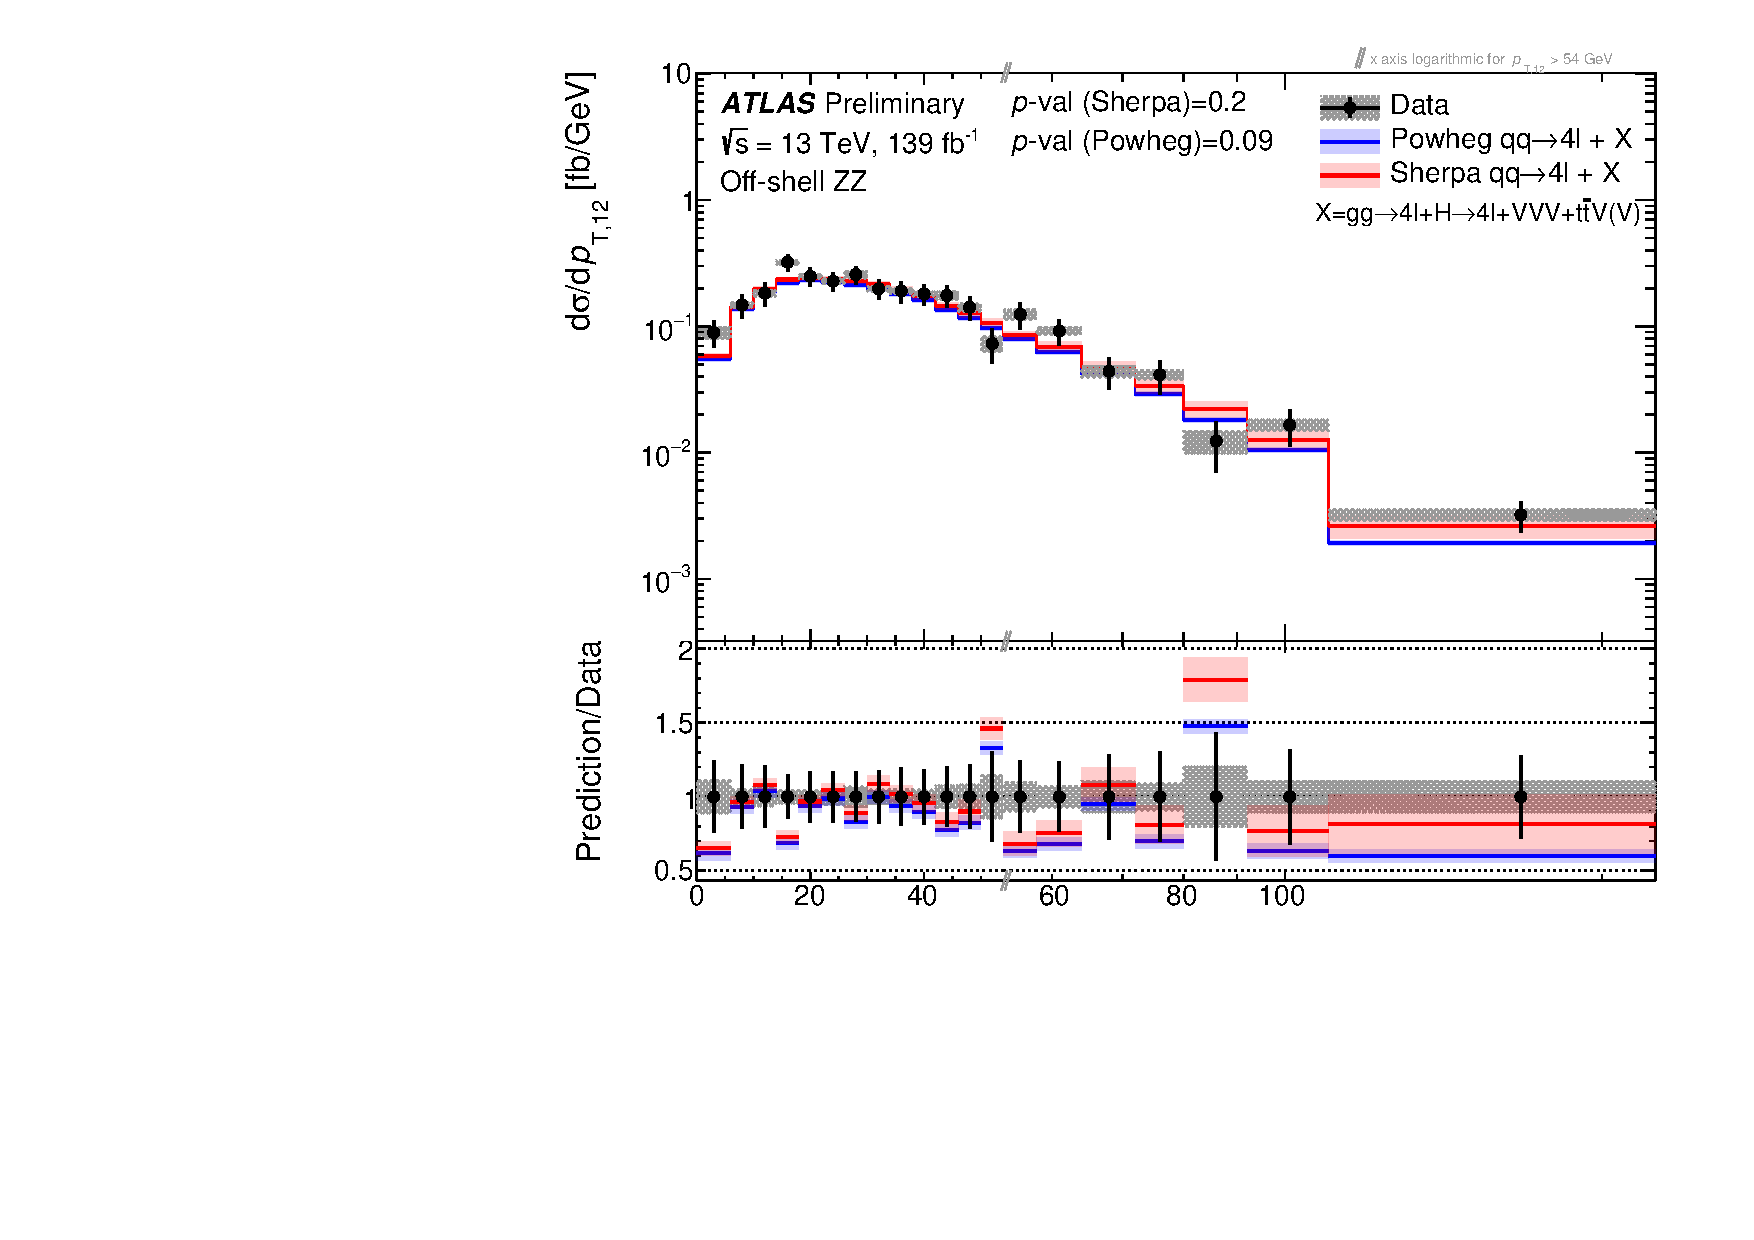
\includegraphics[width=.95\linewidth]{Figures/m4l/UnfoldedResults/linlog_Unfolded_Data_pt12_m4loffshell.pdf}  \caption{Off-shell $\Z\Z$ region}\label{fig:sub-third}
    \end{subfigure}
    \begin{subfigure}{.49\textwidth}\centering
      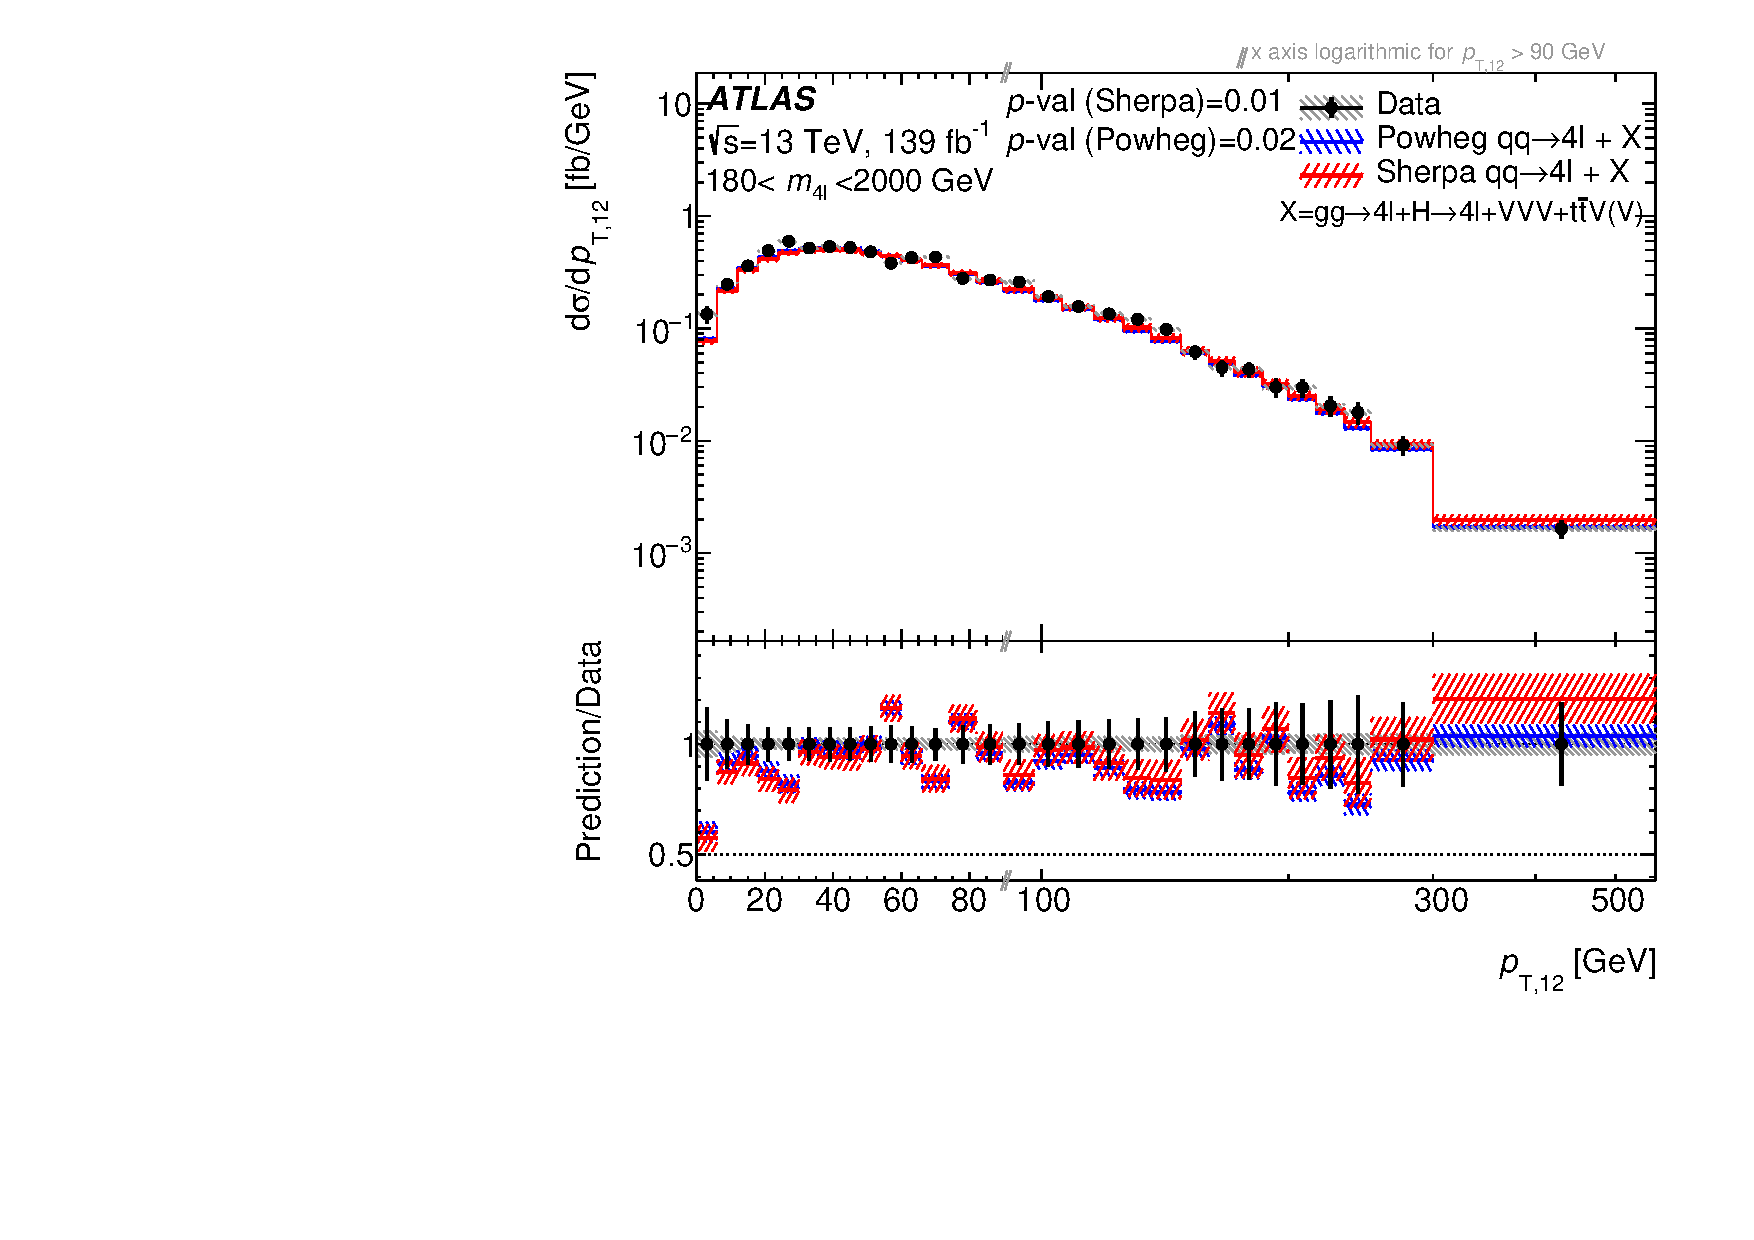
\includegraphics[width=.95\linewidth]{Figures/m4l/UnfoldedResults/linlog_Unfolded_Data_pt12_m4l180-2000.pdf}  \caption{On-shell $\Z\Z$ region}\label{fig:sub-fourth}
    \end{subfigure}
    \caption{Differential cross-section as a function of \ptZOne{} in the four
        \mFourL{} regions. The measured data (black points) are  compared with the SM prediction using either \SHERPA{} (red, with red hashed band for the uncertainty) or \POWHEG{} + \pythia{} (blue, with blue hashed band for the uncertainty) to model the \qqFourL{} contribution. In (b) the contribution from Higgs production is shown in addition to the total SM prediction. The error bars on the data points give the total uncertainty and the grey hashed band gives the systematic uncertainty. \Pvalue{} The  lower panel shows the ratio of the SM predictions to the data.}
    \label{fig:pt12_m4l}
\end{figure}

%% pt34 vs m4l
\begin{figure}[H]
    \begin{subfigure}{.49\textwidth}\centering
      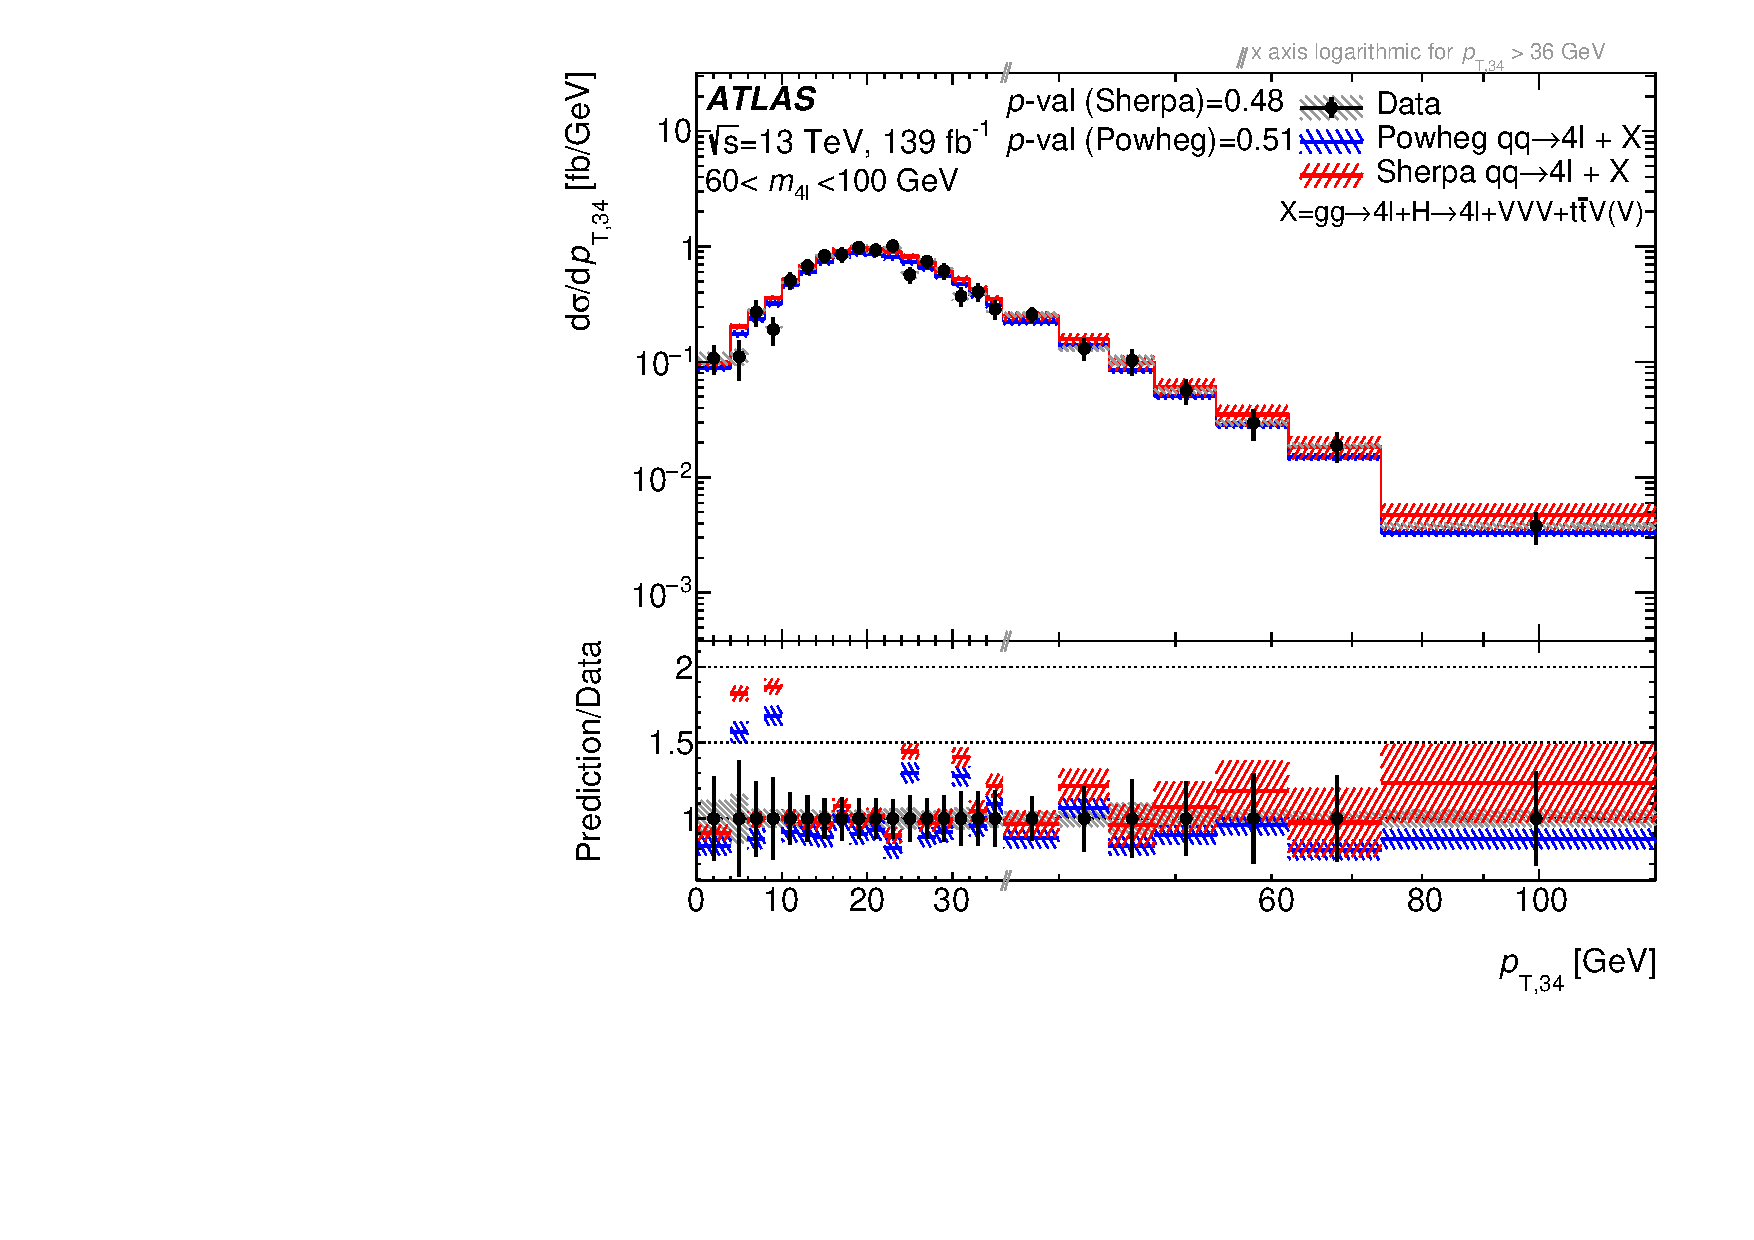
\includegraphics[width=.95\linewidth]{Figures/m4l/UnfoldedResults/linlog_Unfolded_Data_pt34_m4l60-100.pdf}\caption{\ZFourL \ region}\label{fig:sub-first}
    \end{subfigure}
    \begin{subfigure}{.49\textwidth}\centering
      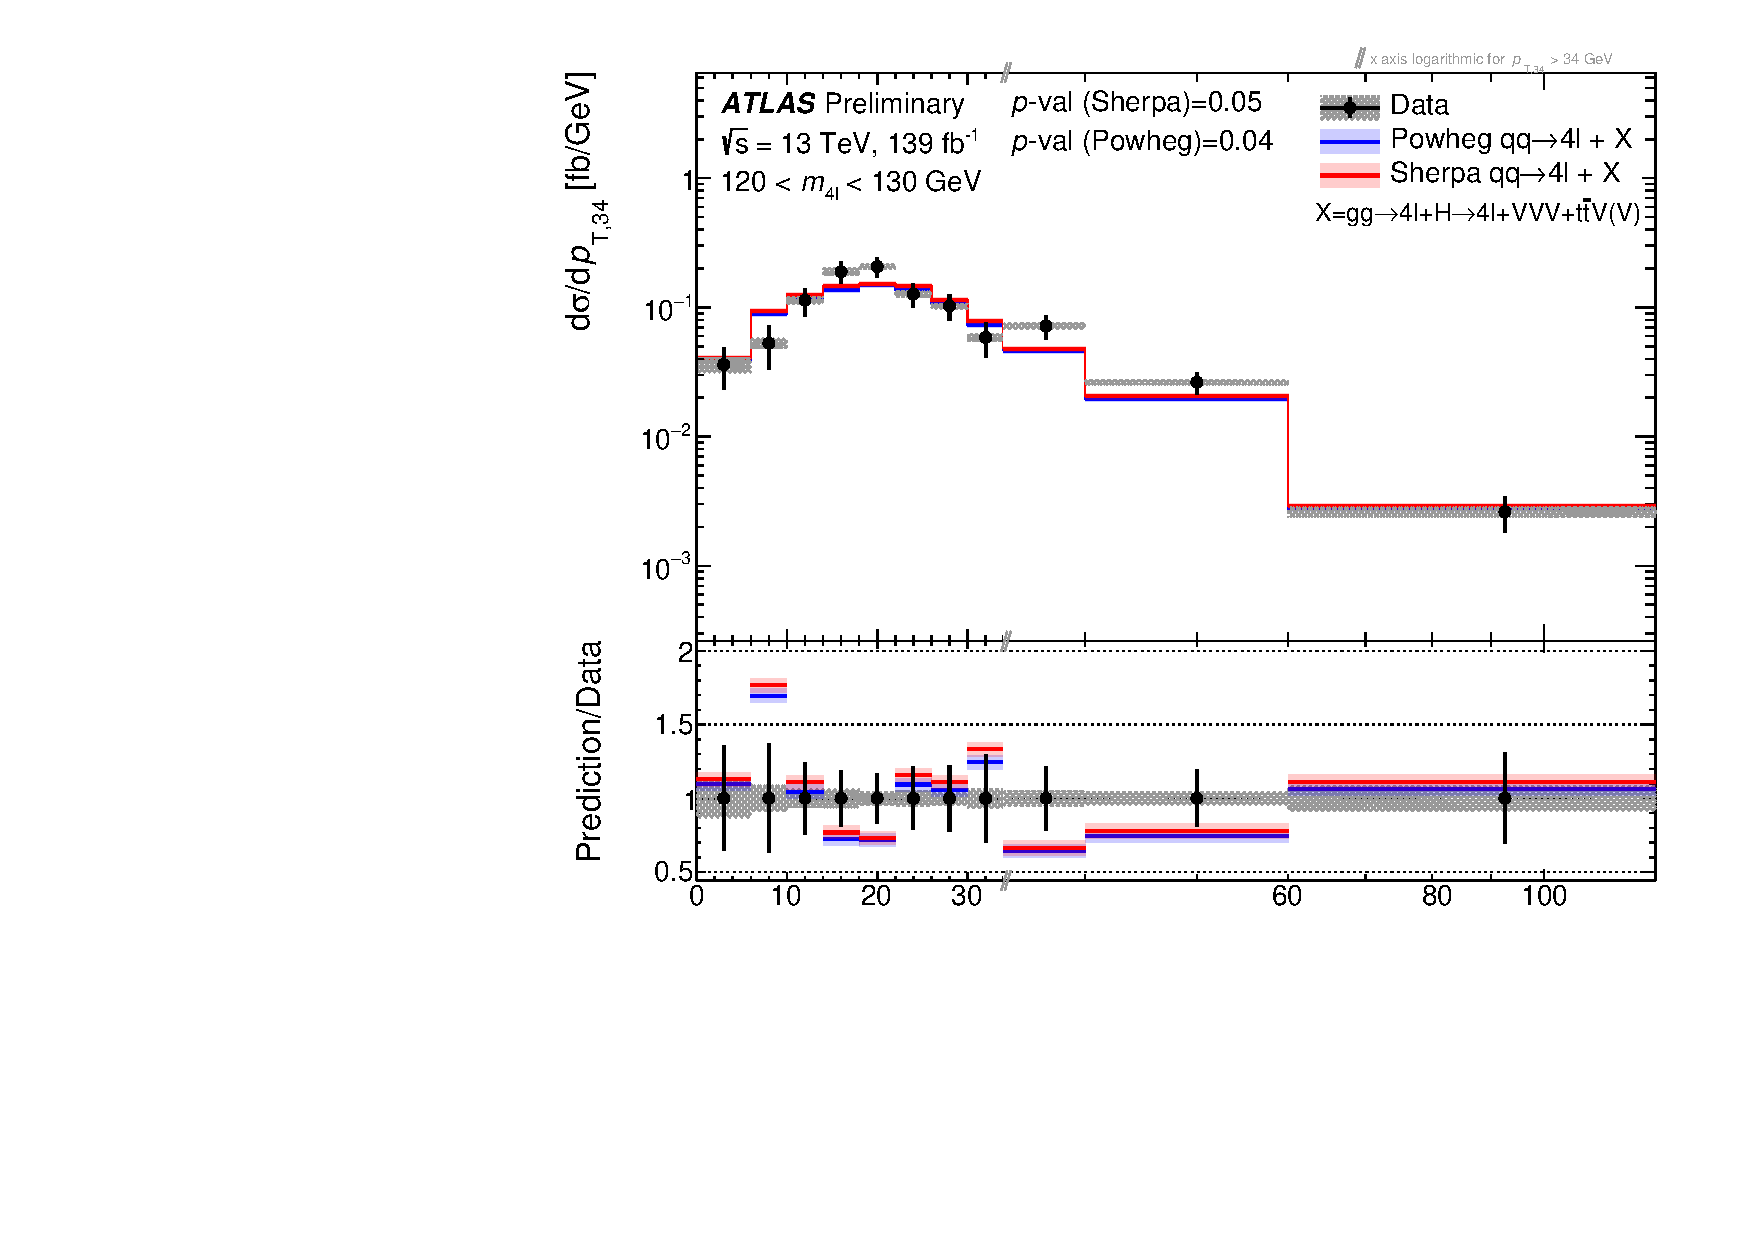
\includegraphics[width=.95\linewidth]{Figures/m4l/UnfoldedResults/linlog_Unfolded_Data_pt34_m4l120-130.pdf} \caption{\HFourL \ region}\label{fig:sub-second}
    \end{subfigure}
    \begin{subfigure}{.49\textwidth}\centering
      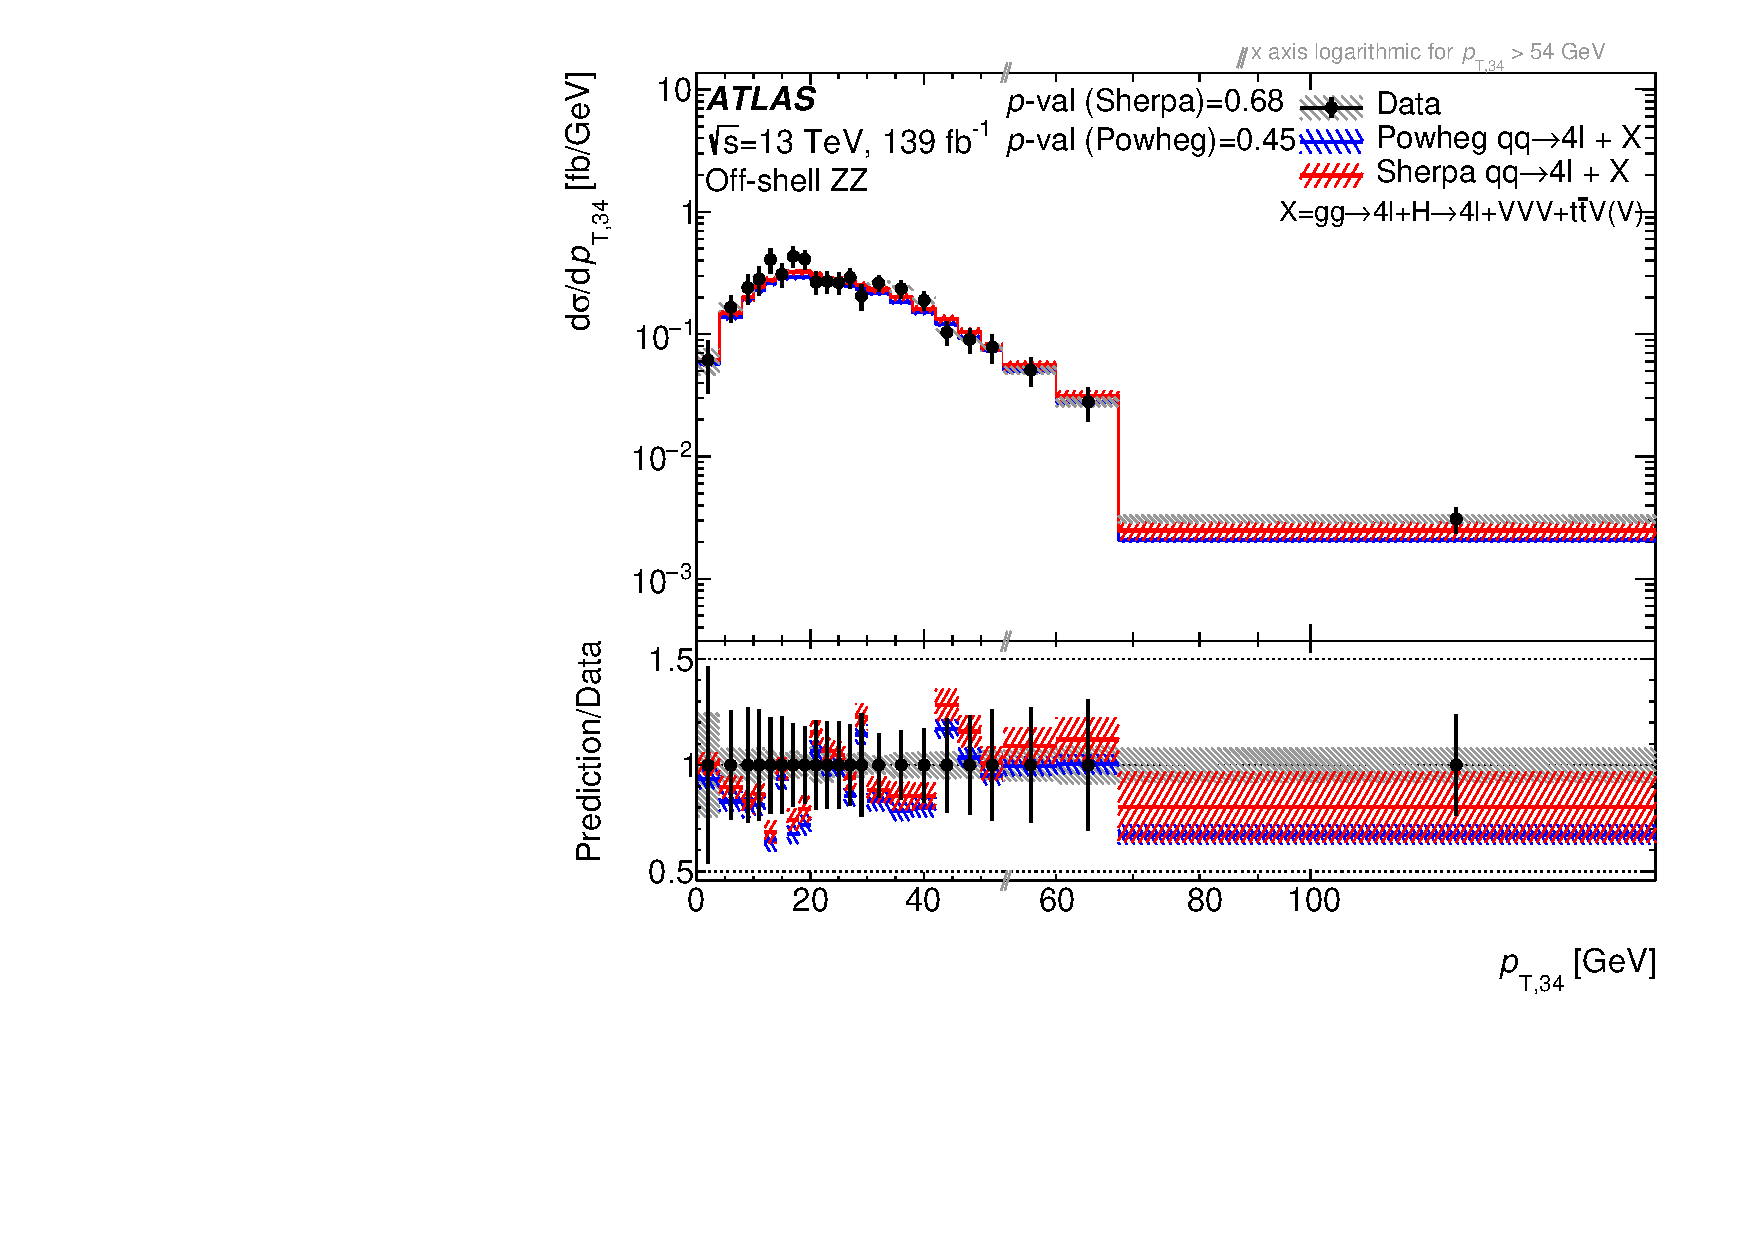
\includegraphics[width=.95\linewidth]{Figures/m4l/UnfoldedResults/linlog_Unfolded_Data_pt34_m4loffshell.pdf}  \caption{Off-shell $\Z\Z$ region}\label{fig:sub-third}
    \end{subfigure}
    \begin{subfigure}{.49\textwidth}\centering
      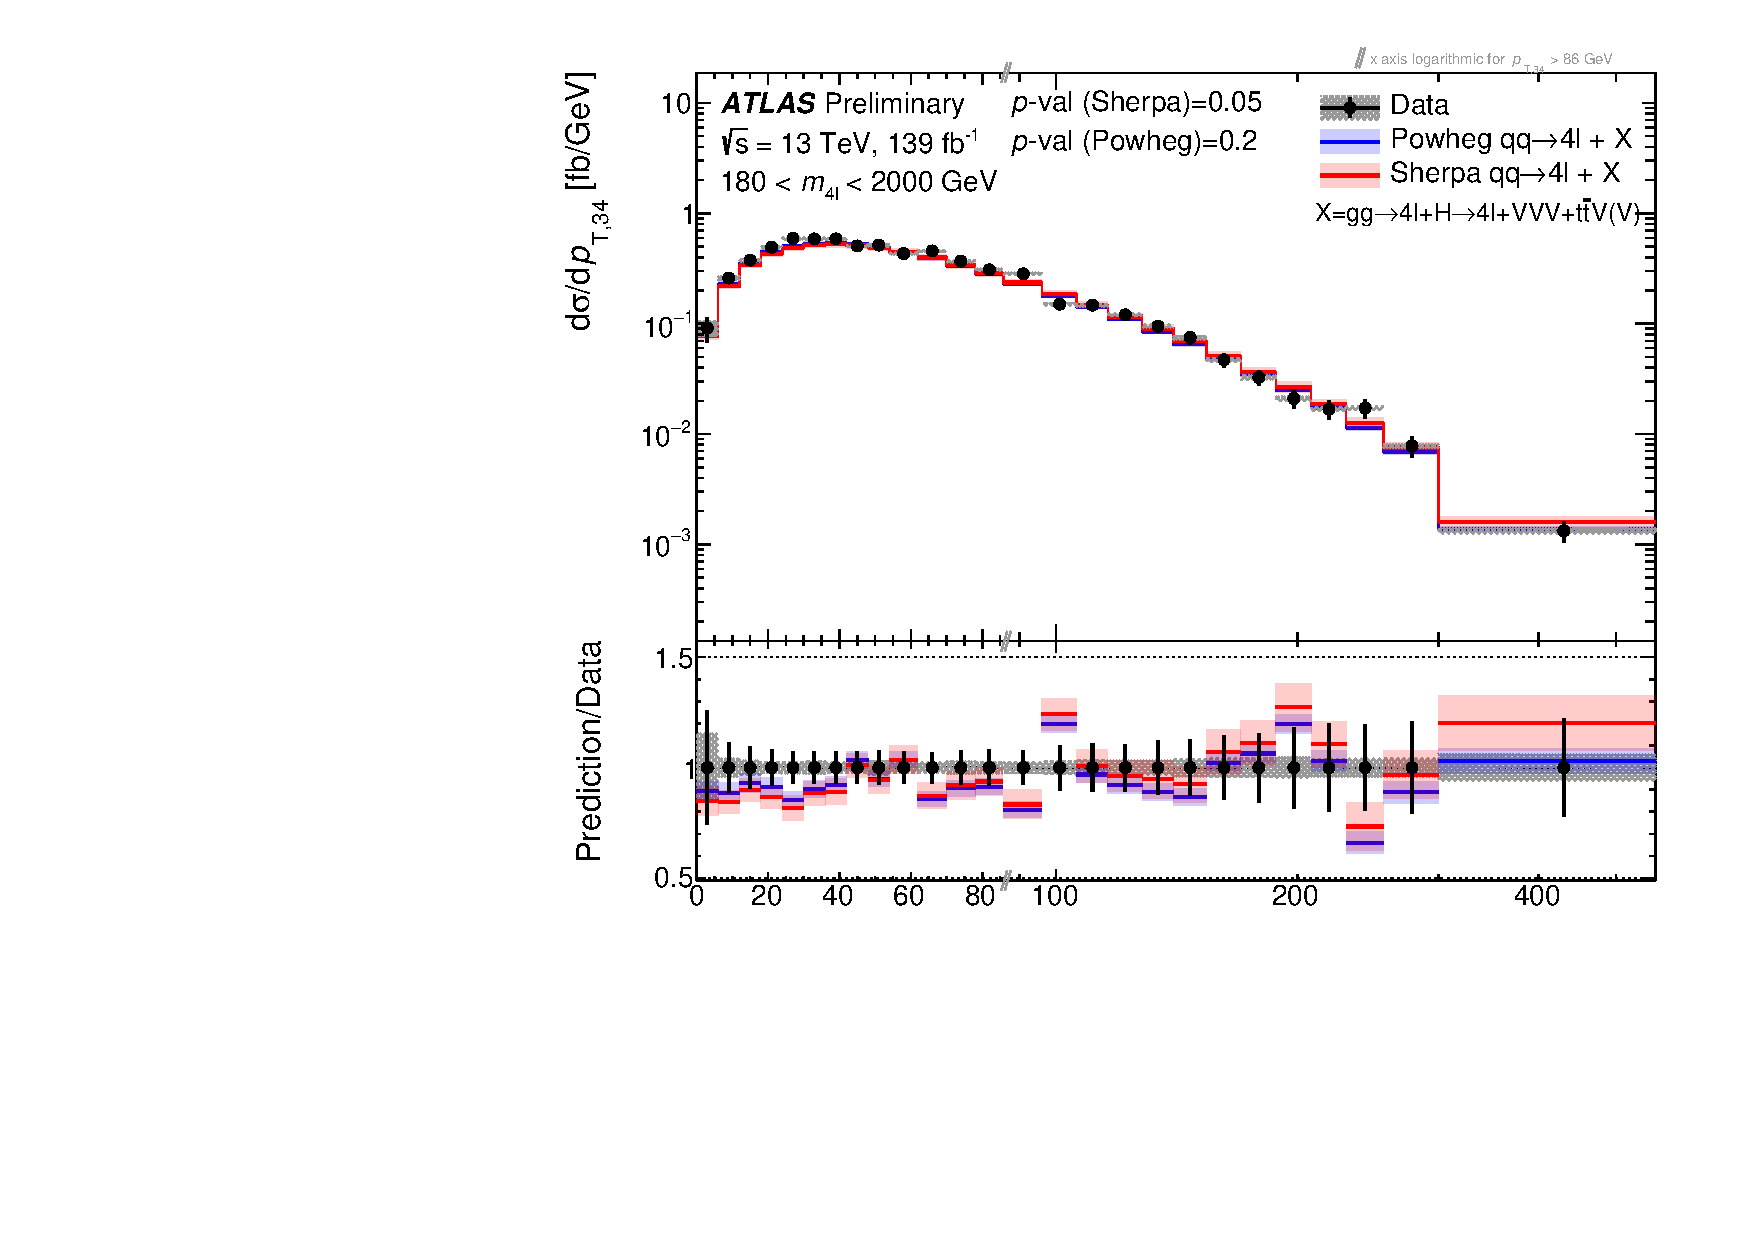
\includegraphics[width=.95\linewidth]{Figures/m4l/UnfoldedResults/linlog_Unfolded_Data_pt34_m4l180-2000.pdf}  \caption{On-shell $\Z\Z$ region}\label{fig:sub-fourth}
    \end{subfigure}
    \caption{Differential cross-section as a function of \ptZTwo{} in the four
        \mFourL{} regions. The measured data (black points) are  compared with the SM prediction using either \SHERPA{} (red, with red hashed band for the uncertainty) or \POWHEG{} + \pythia{} (blue, with blue hashed band for the uncertainty) to model the \qqFourL{} contribution. The error bars on the data points give the total uncertainty and the grey hashed band gives the systematic uncertainty. \Pvalue{} The  lower panel shows the ratio of the SM predictions to the data.}
    \label{fig:pt34_m4l}
\end{figure}

%% cosThetaStar1 vs m4l
\begin{figure}[H]
    \begin{subfigure}{.49\textwidth}\centering
      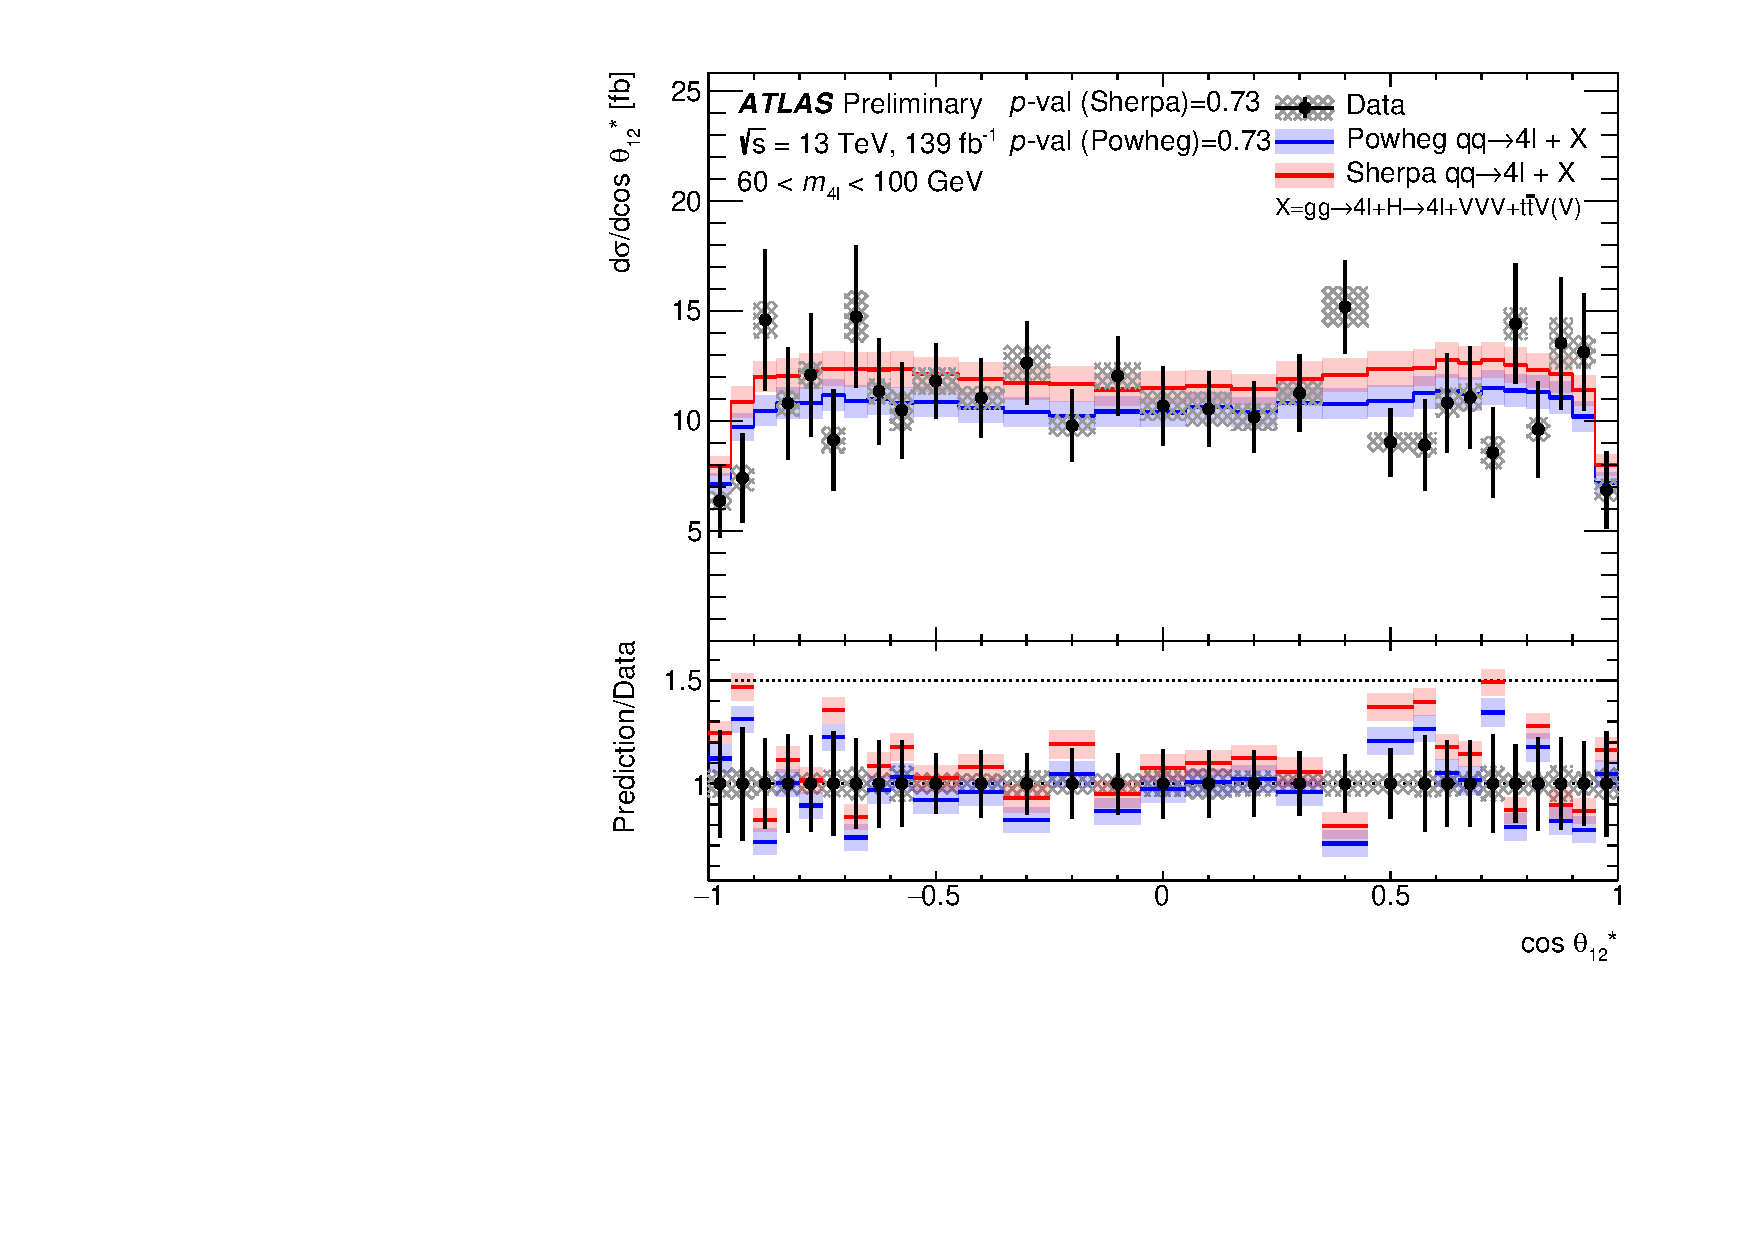
\includegraphics[width=.95\linewidth]{Figures/m4l/UnfoldedResults/linY_Unfolded_Data_cosThetaStar1_m4l60-100.pdf}\caption{\ZFourL \ region}\label{fig:sub-first}
    \end{subfigure}
    \begin{subfigure}{.49\textwidth}\centering
      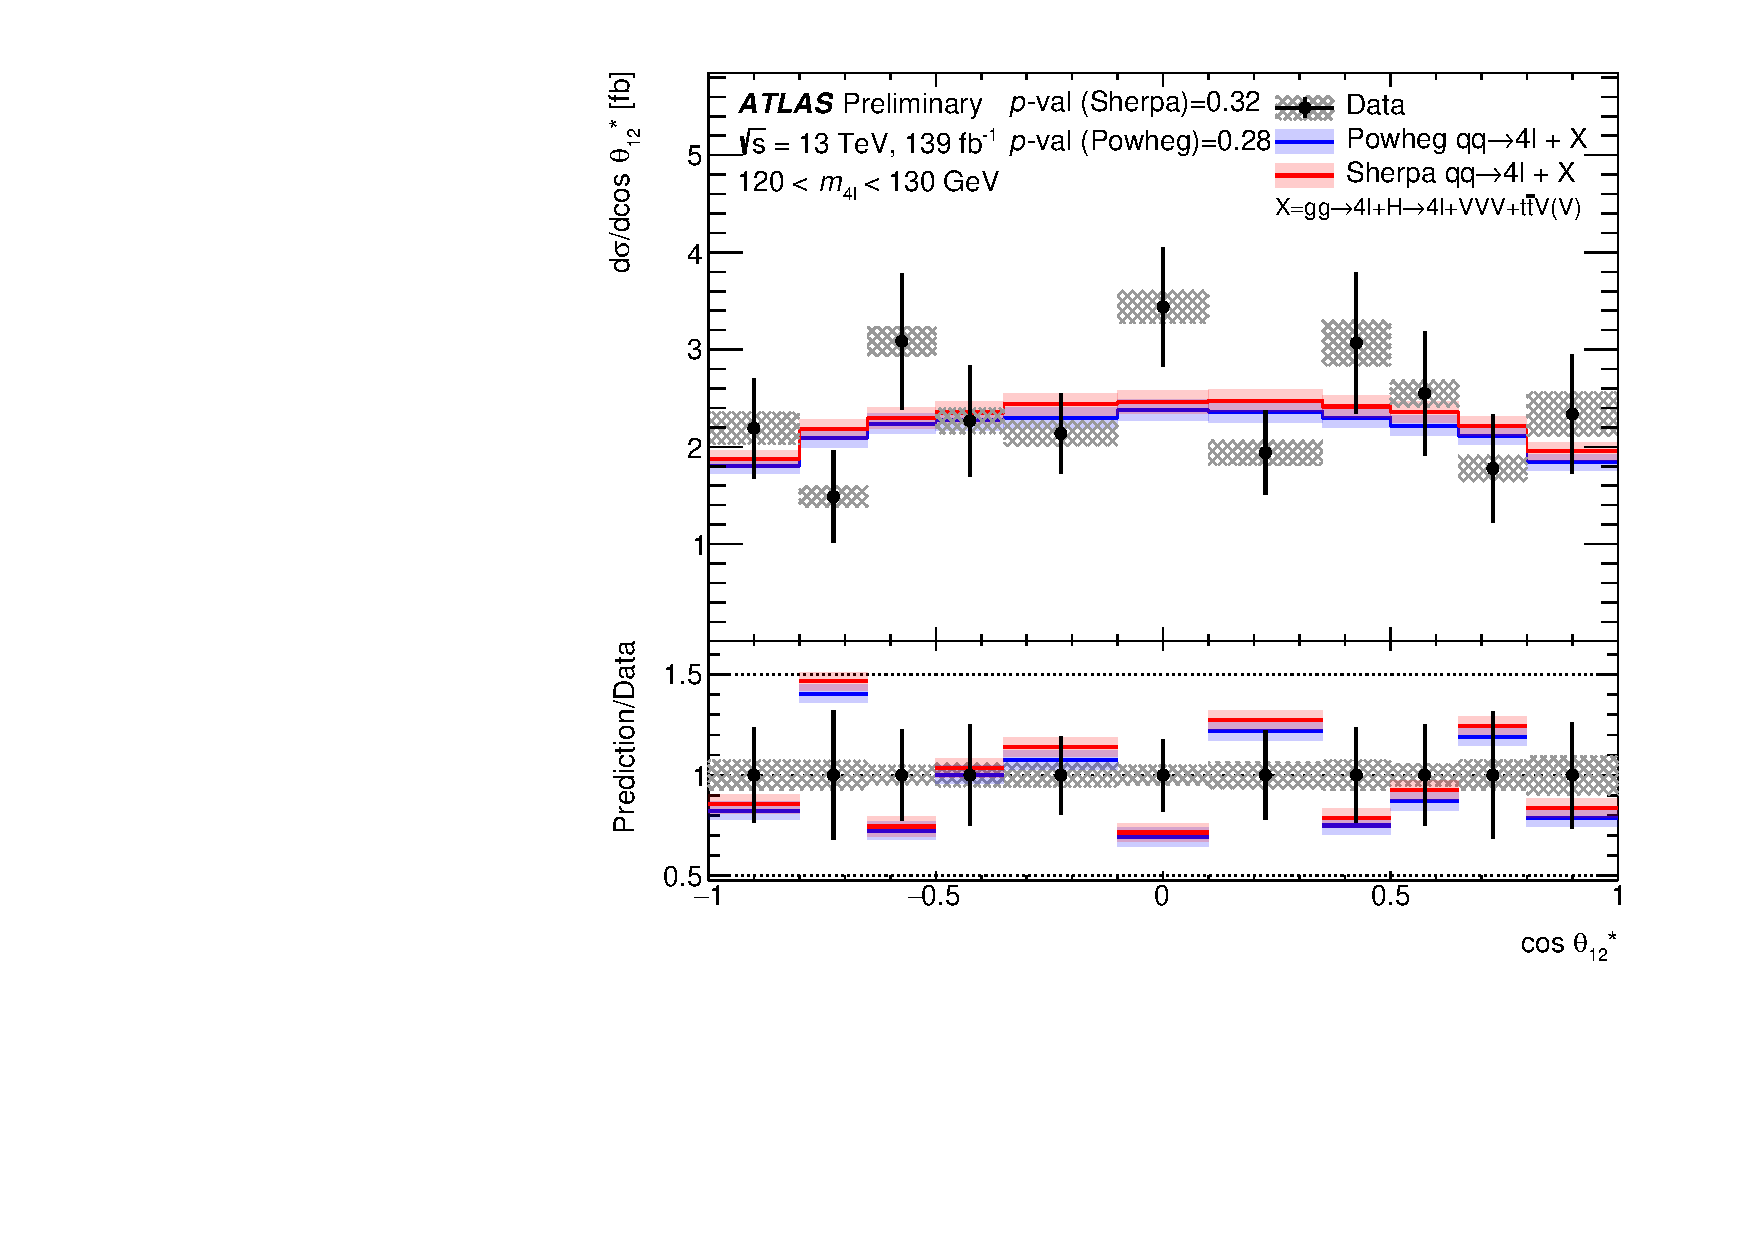
\includegraphics[width=.95\linewidth]{Figures/m4l/UnfoldedResults/linY_Unfolded_Data_cosThetaStar1_m4l120-130.pdf} \caption{\HFourL \ region}\label{fig:sub-second}
    \end{subfigure}
    \begin{subfigure}{.49\textwidth}\centering
      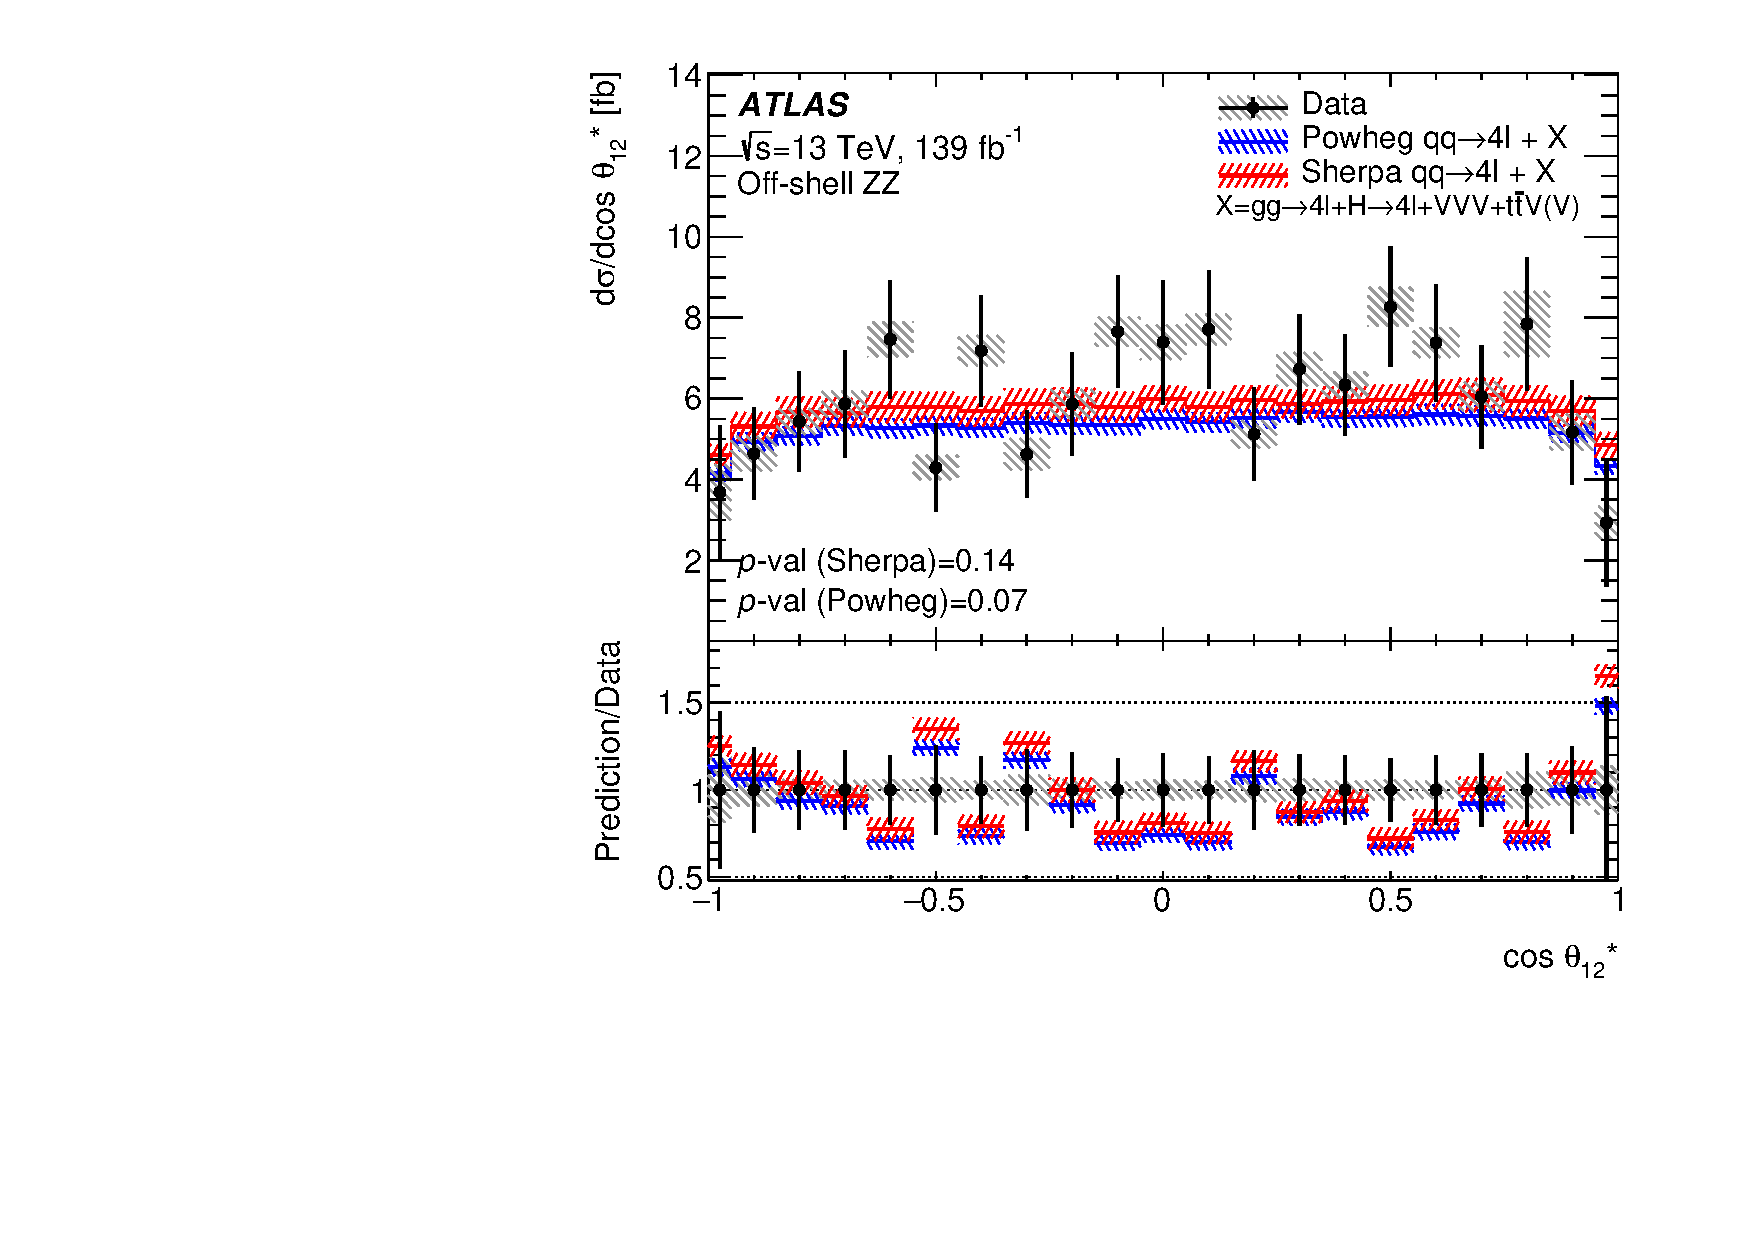
\includegraphics[width=.95\linewidth]{Figures/m4l/UnfoldedResults/linY_Unfolded_Data_cosThetaStar1_m4loffshell.pdf}  \caption{Off-shell $\Z\Z$ region}\label{fig:sub-third}
    \end{subfigure}
    \begin{subfigure}{.49\textwidth}\centering
      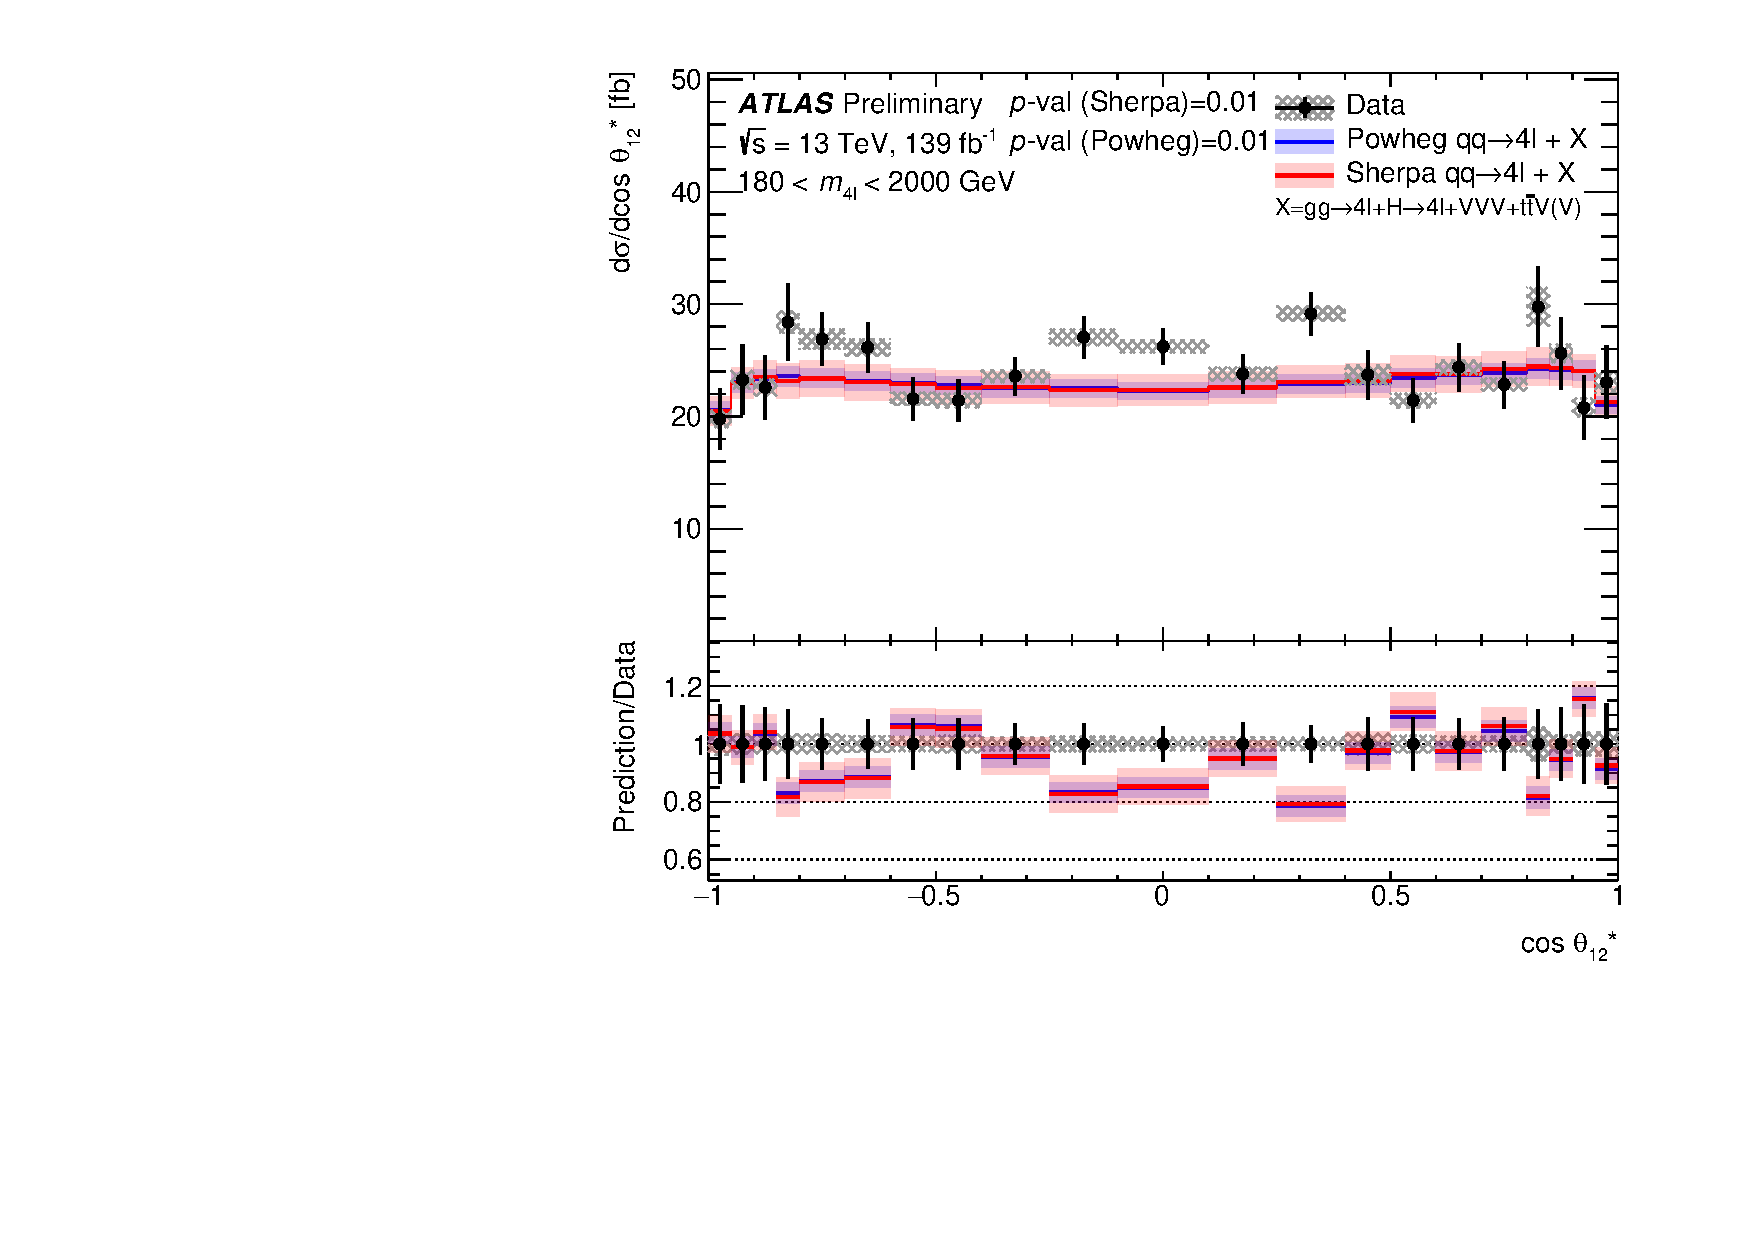
\includegraphics[width=.95\linewidth]{Figures/m4l/UnfoldedResults/linY_Unfolded_Data_cosThetaStar1_m4l180-2000.pdf}  \caption{On-shell $\Z\Z$ region}\label{fig:sub-fourth}
    \end{subfigure}
    \caption{Differential cross-section as a function of \CTSOneTwo{} in the four
        \mFourL{} regions. The measured data (black points) are  compared with the SM prediction using either \SHERPA{} (red, with red hashed band for the uncertainty) or \POWHEG{} + \pythia{} (blue, with blue hashed band for the uncertainty) to model the \qqFourL{} contribution. The error bars on the data points give the total uncertainty and the grey hashed band gives the systematic uncertainty. \Pvalue{} The  lower panel shows the ratio of the SM predictions to the data.}
    \label{fig:cts12_m4l}
\end{figure}

%% cosThetaStar3 vs m4l
\begin{figure}[H]
    \begin{subfigure}{.49\textwidth}\centering
      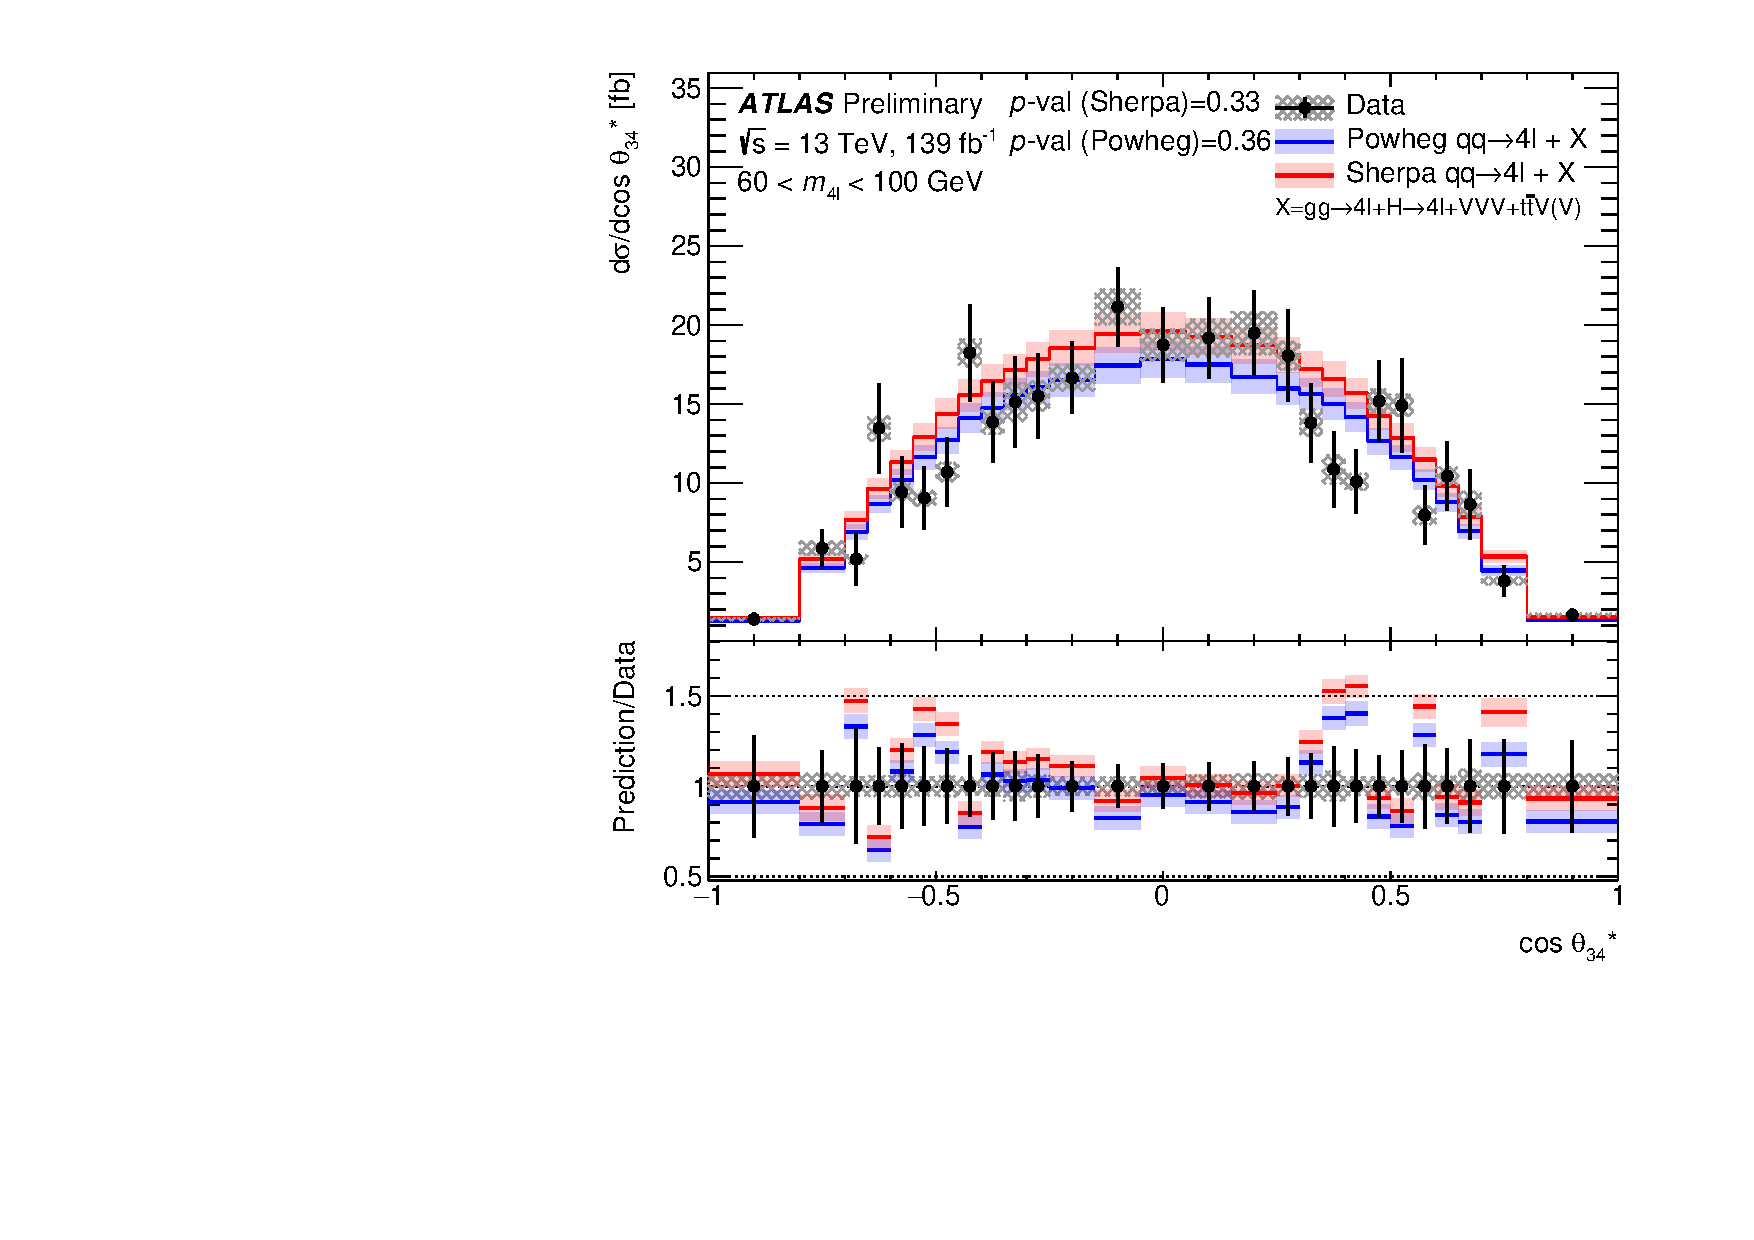
\includegraphics[width=.95\linewidth]{Figures/m4l/UnfoldedResults/linY_Unfolded_Data_cosThetaStar3_m4l60-100.pdf}\caption{\ZFourL \ region}\label{fig:sub-first}
    \end{subfigure}
    \begin{subfigure}{.49\textwidth}\centering
      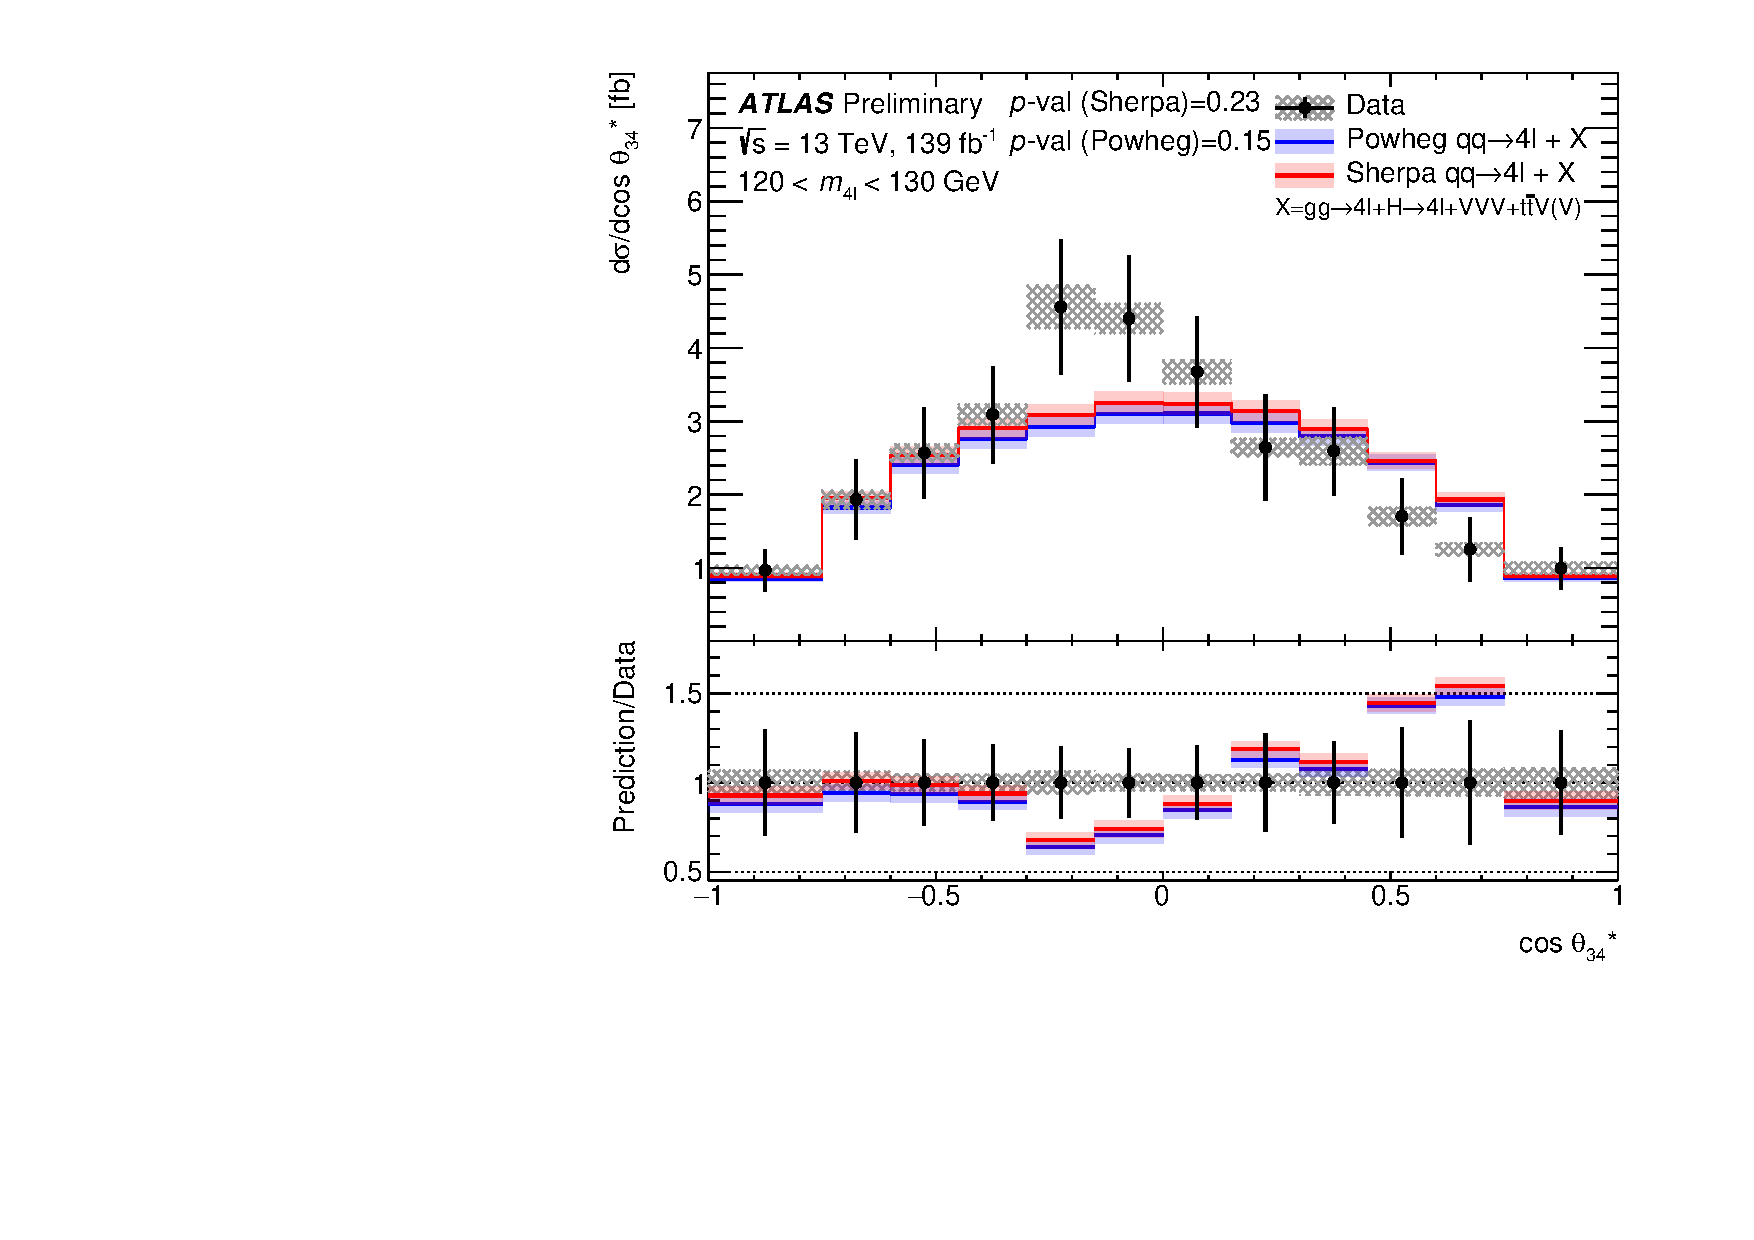
\includegraphics[width=.95\linewidth]{Figures/m4l/UnfoldedResults/linY_Unfolded_Data_cosThetaStar3_m4l120-130.pdf} \caption{\HFourL \ region}\label{fig:sub-second}
    \end{subfigure}
    \begin{subfigure}{.49\textwidth}\centering
      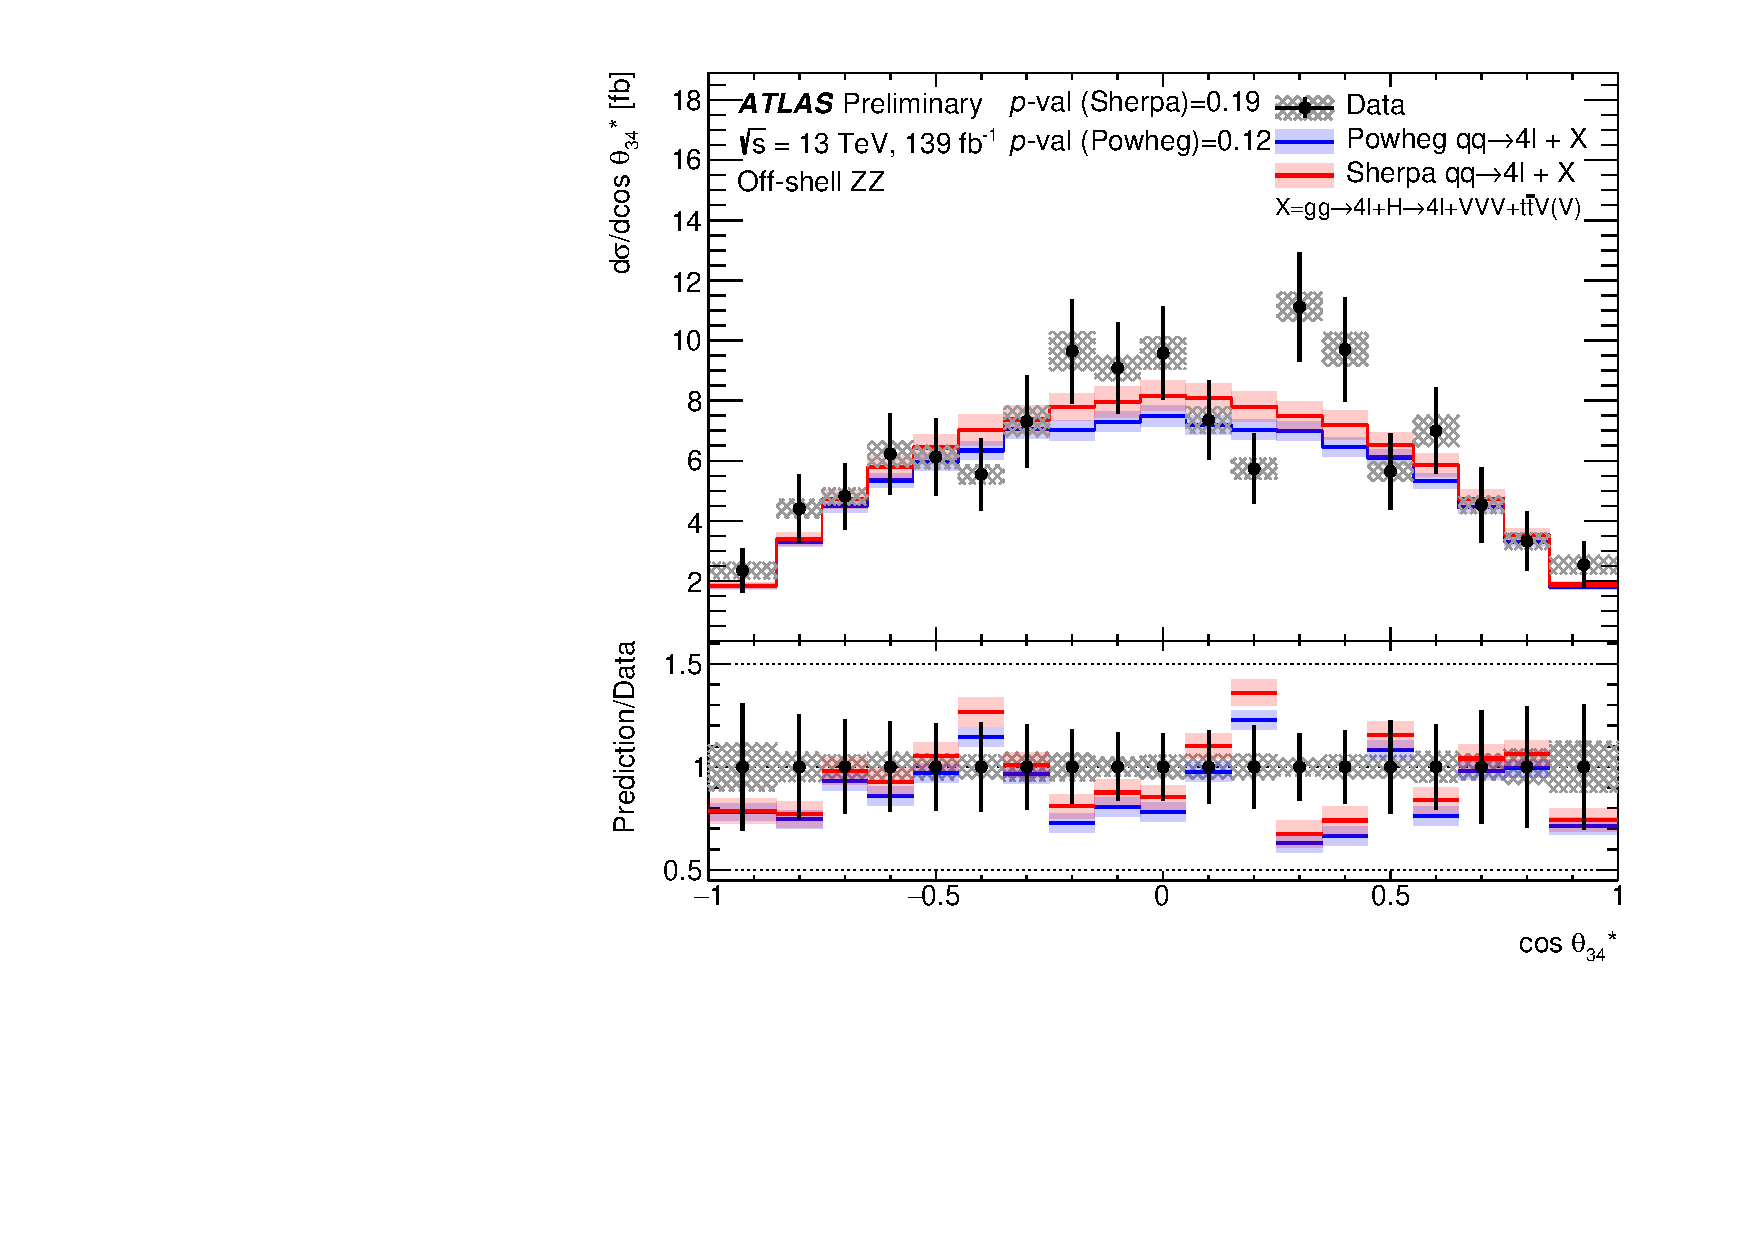
\includegraphics[width=.95\linewidth]{Figures/m4l/UnfoldedResults/linY_Unfolded_Data_cosThetaStar3_m4loffshell.pdf}  \caption{Off-shell $\Z\Z$ region}\label{fig:sub-third}
    \end{subfigure}
    \begin{subfigure}{.49\textwidth}\centering
      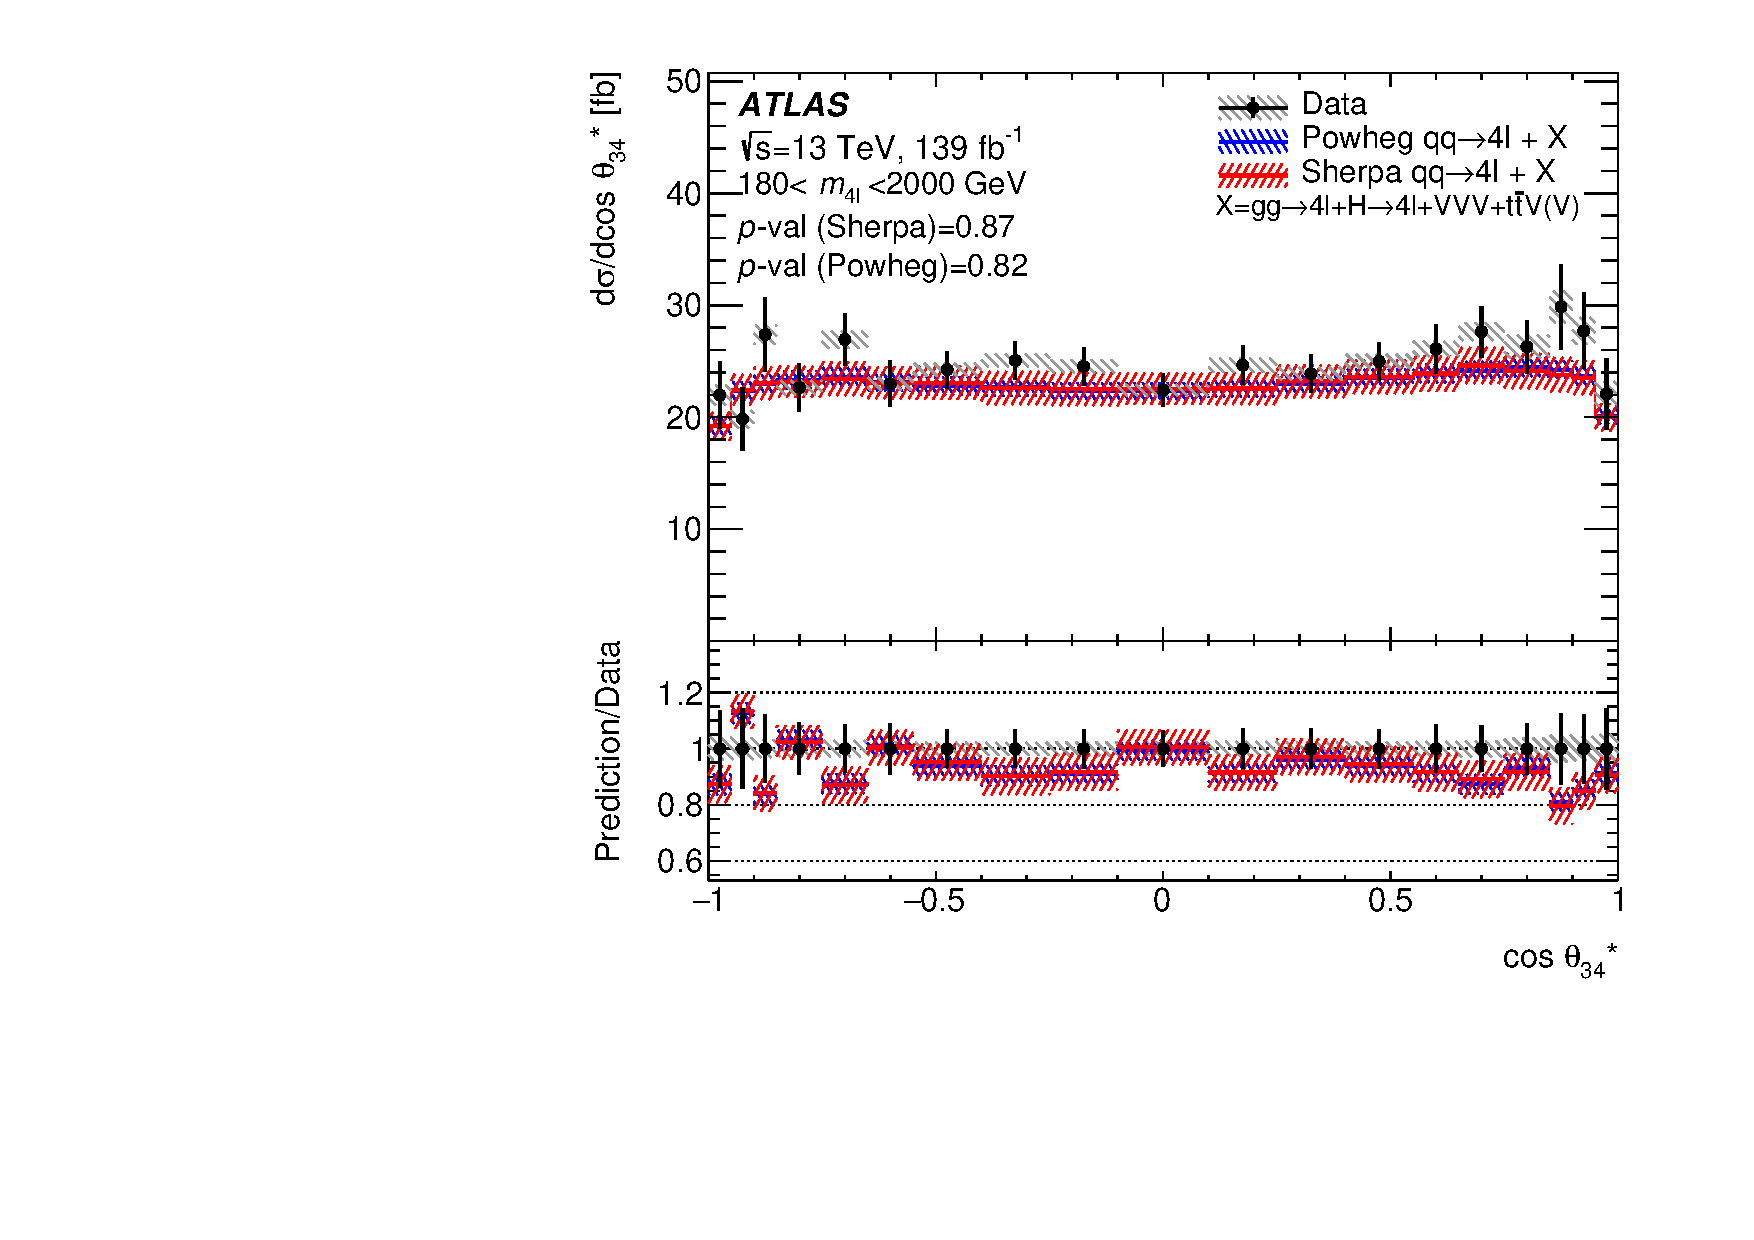
\includegraphics[width=.95\linewidth]{Figures/m4l/UnfoldedResults/linY_Unfolded_Data_cosThetaStar3_m4l180-2000.pdf}  \caption{On-shell $\Z\Z$ region}\label{fig:sub-fourth}
    \end{subfigure}
    \caption{Differential cross-section as a function of \CTSThreeFour{} in the four
        \mFourL{} regions. The measured data (black points) are  compared with the SM prediction using either \SHERPA{} (red, with red hashed band for the uncertainty) or \POWHEG{} + \pythia{} (blue, with blue hashed band for the uncertainty) to model the \qqFourL{} contribution. The error bars on the data points give the total uncertainty and the grey hashed band gives the systematic uncertainty. \Pvalue{} The  lower panel shows the ratio of the SM predictions to the data.}
    \label{fig:cts34_m4l}
\end{figure}

%% deltaPhiLeptons vs m4l
\begin{figure}[H]
    \begin{subfigure}{.49\textwidth}\centering
      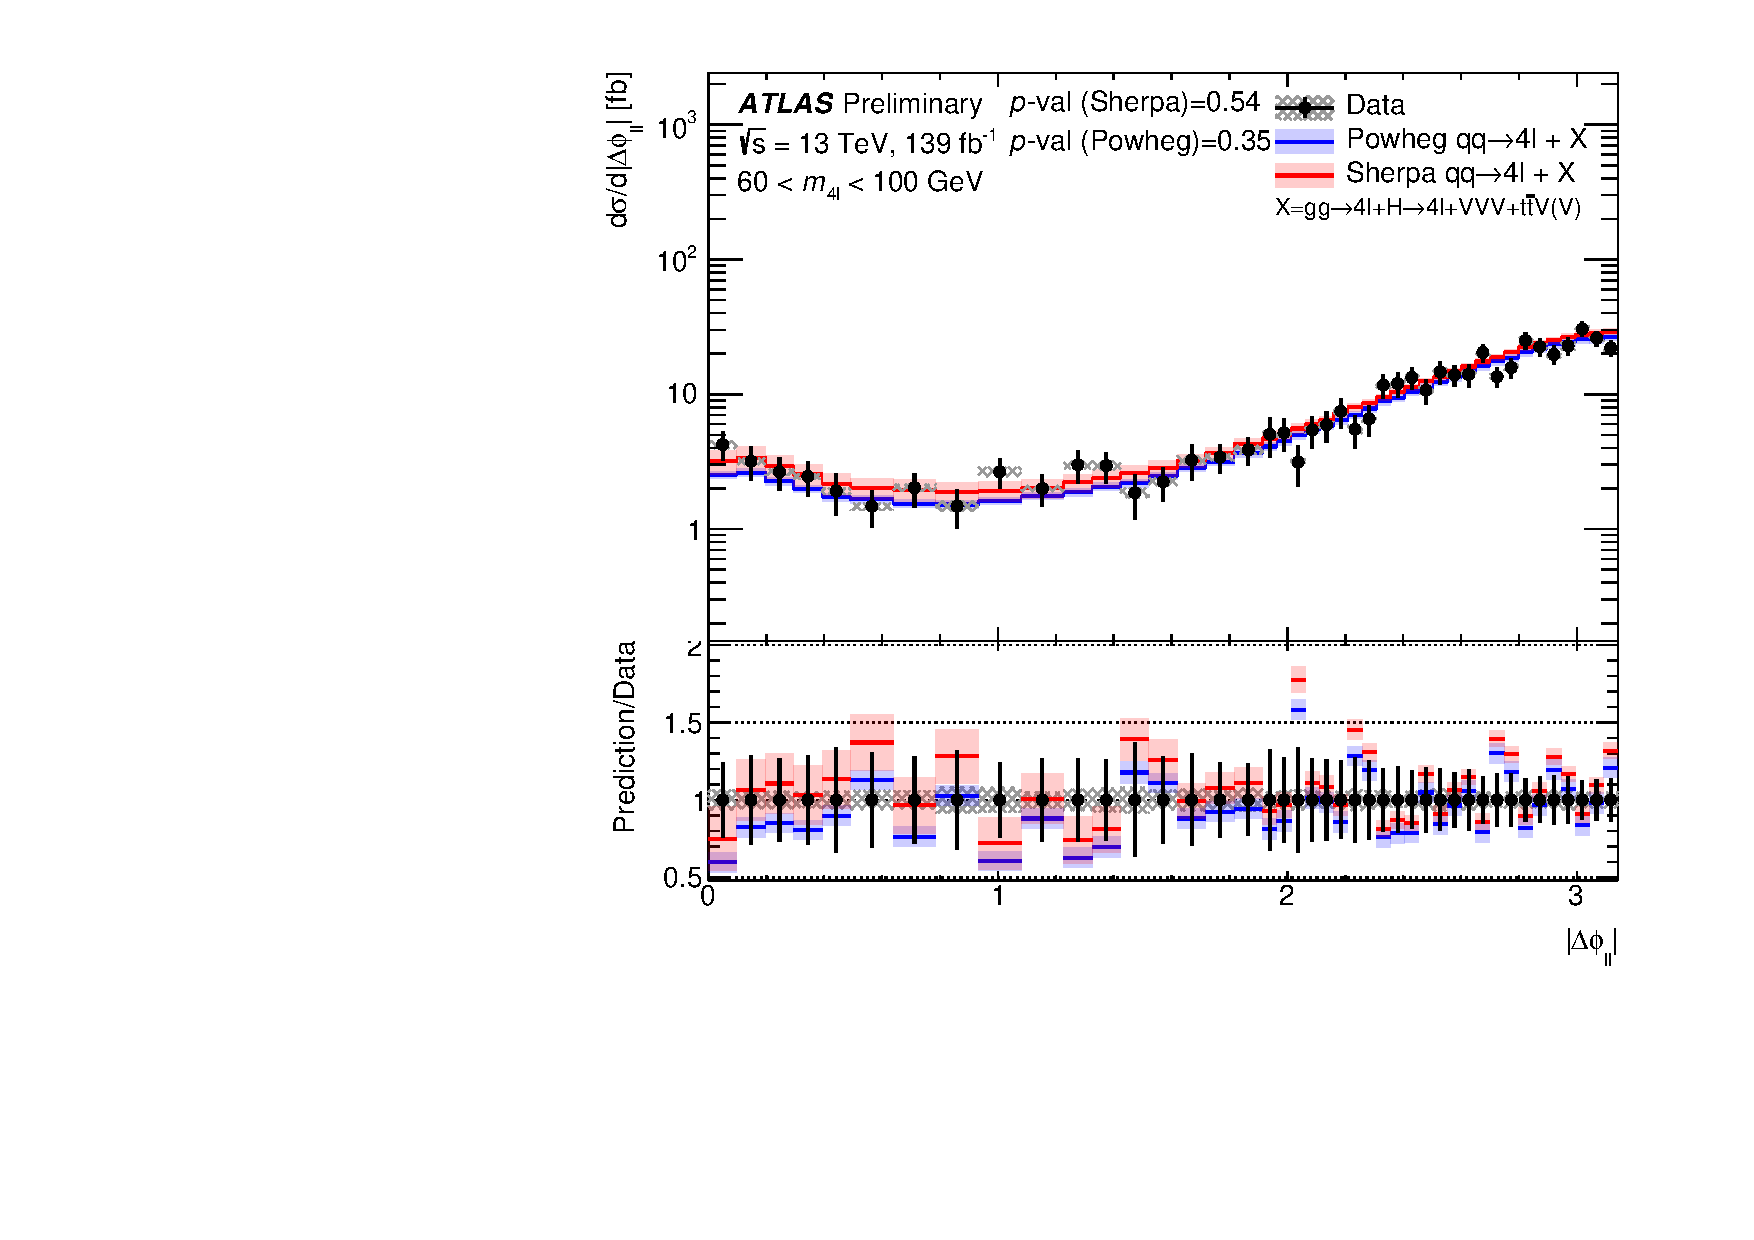
\includegraphics[width=.95\linewidth]{Figures/m4l/UnfoldedResults/Unfolded_Data_deltaPhiLeadingLeptons_m4l60-100.pdf}\caption{\ZFourL \ region}\label{fig:sub-first}
    \end{subfigure}
    \begin{subfigure}{.49\textwidth}\centering
      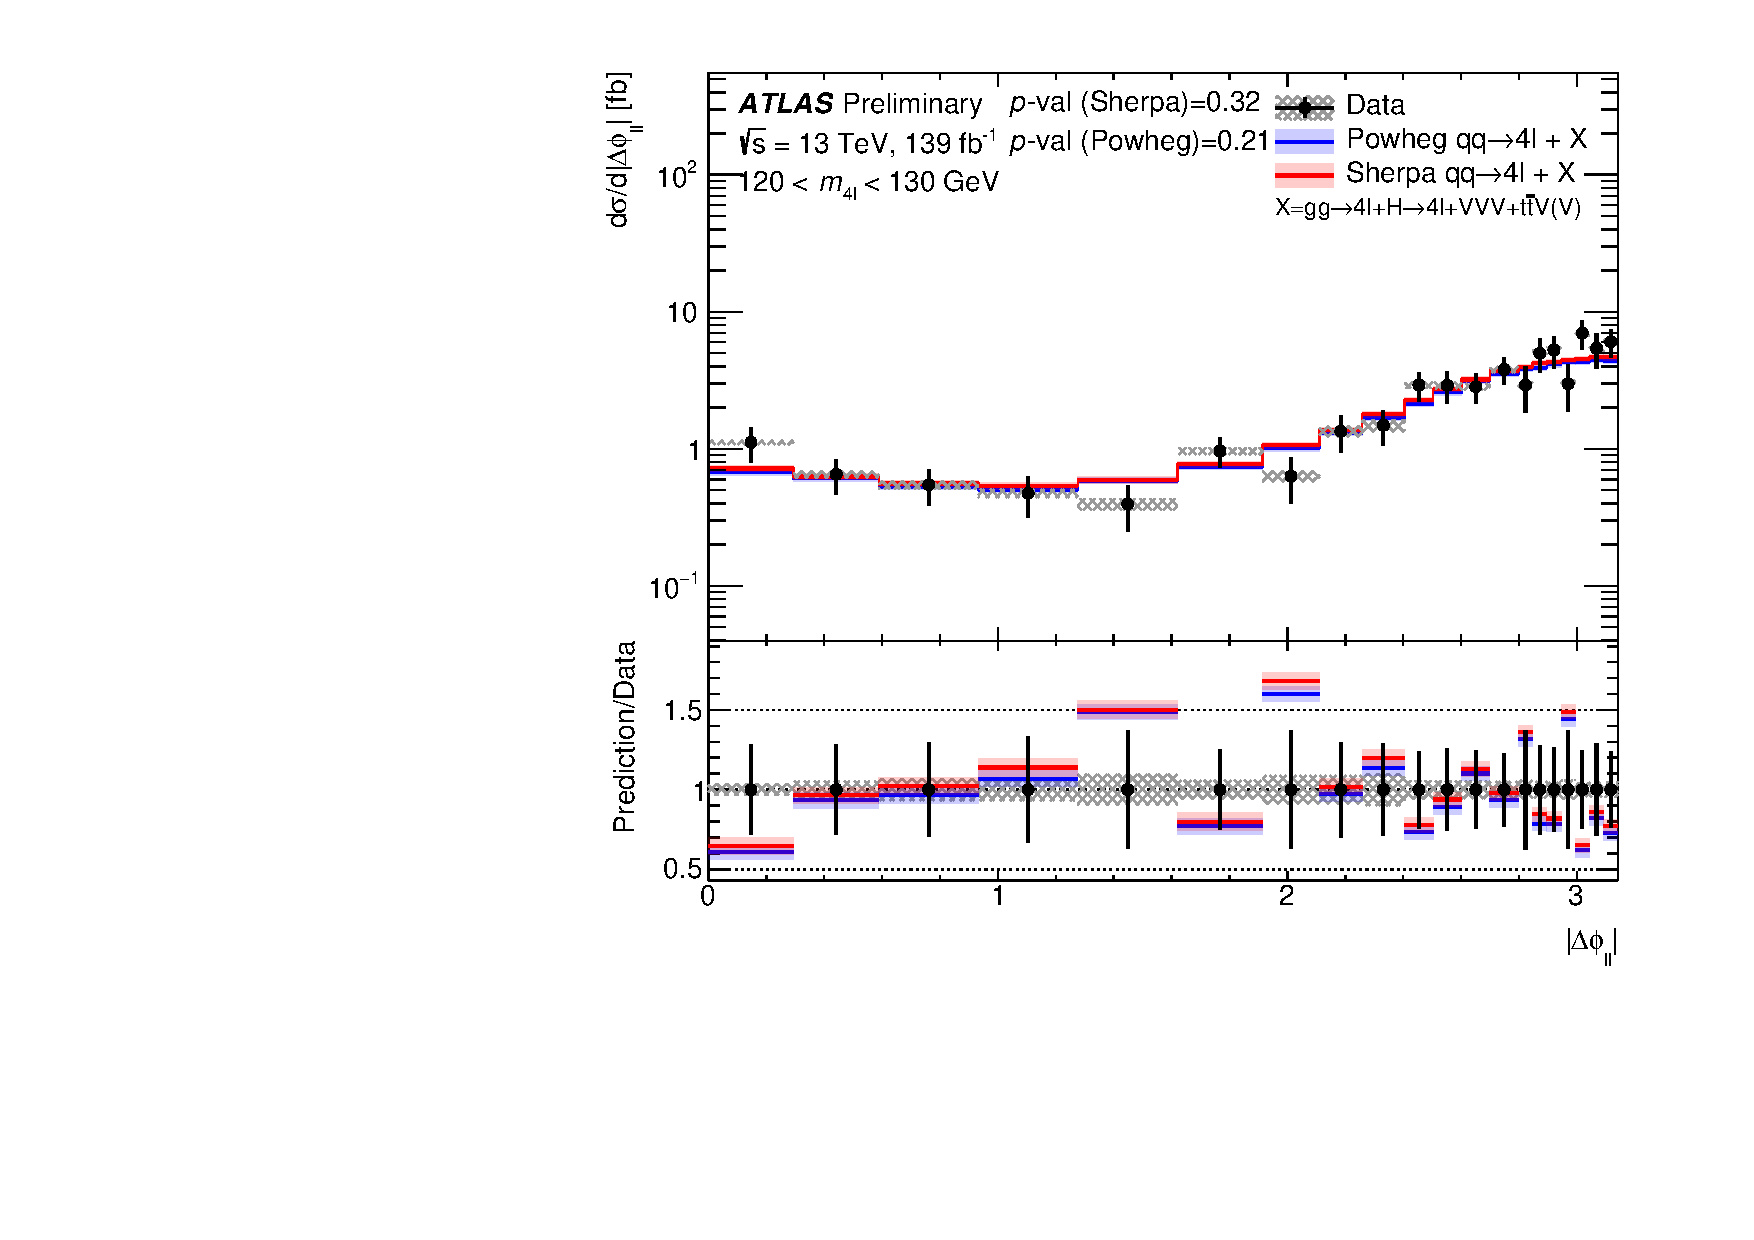
\includegraphics[width=.95\linewidth]{Figures/m4l/UnfoldedResults/Unfolded_Data_deltaPhiLeadingLeptons_m4l120-130.pdf} \caption{\HFourL \ region}\label{fig:sub-second}
    \end{subfigure}
    \begin{subfigure}{.49\textwidth}\centering
      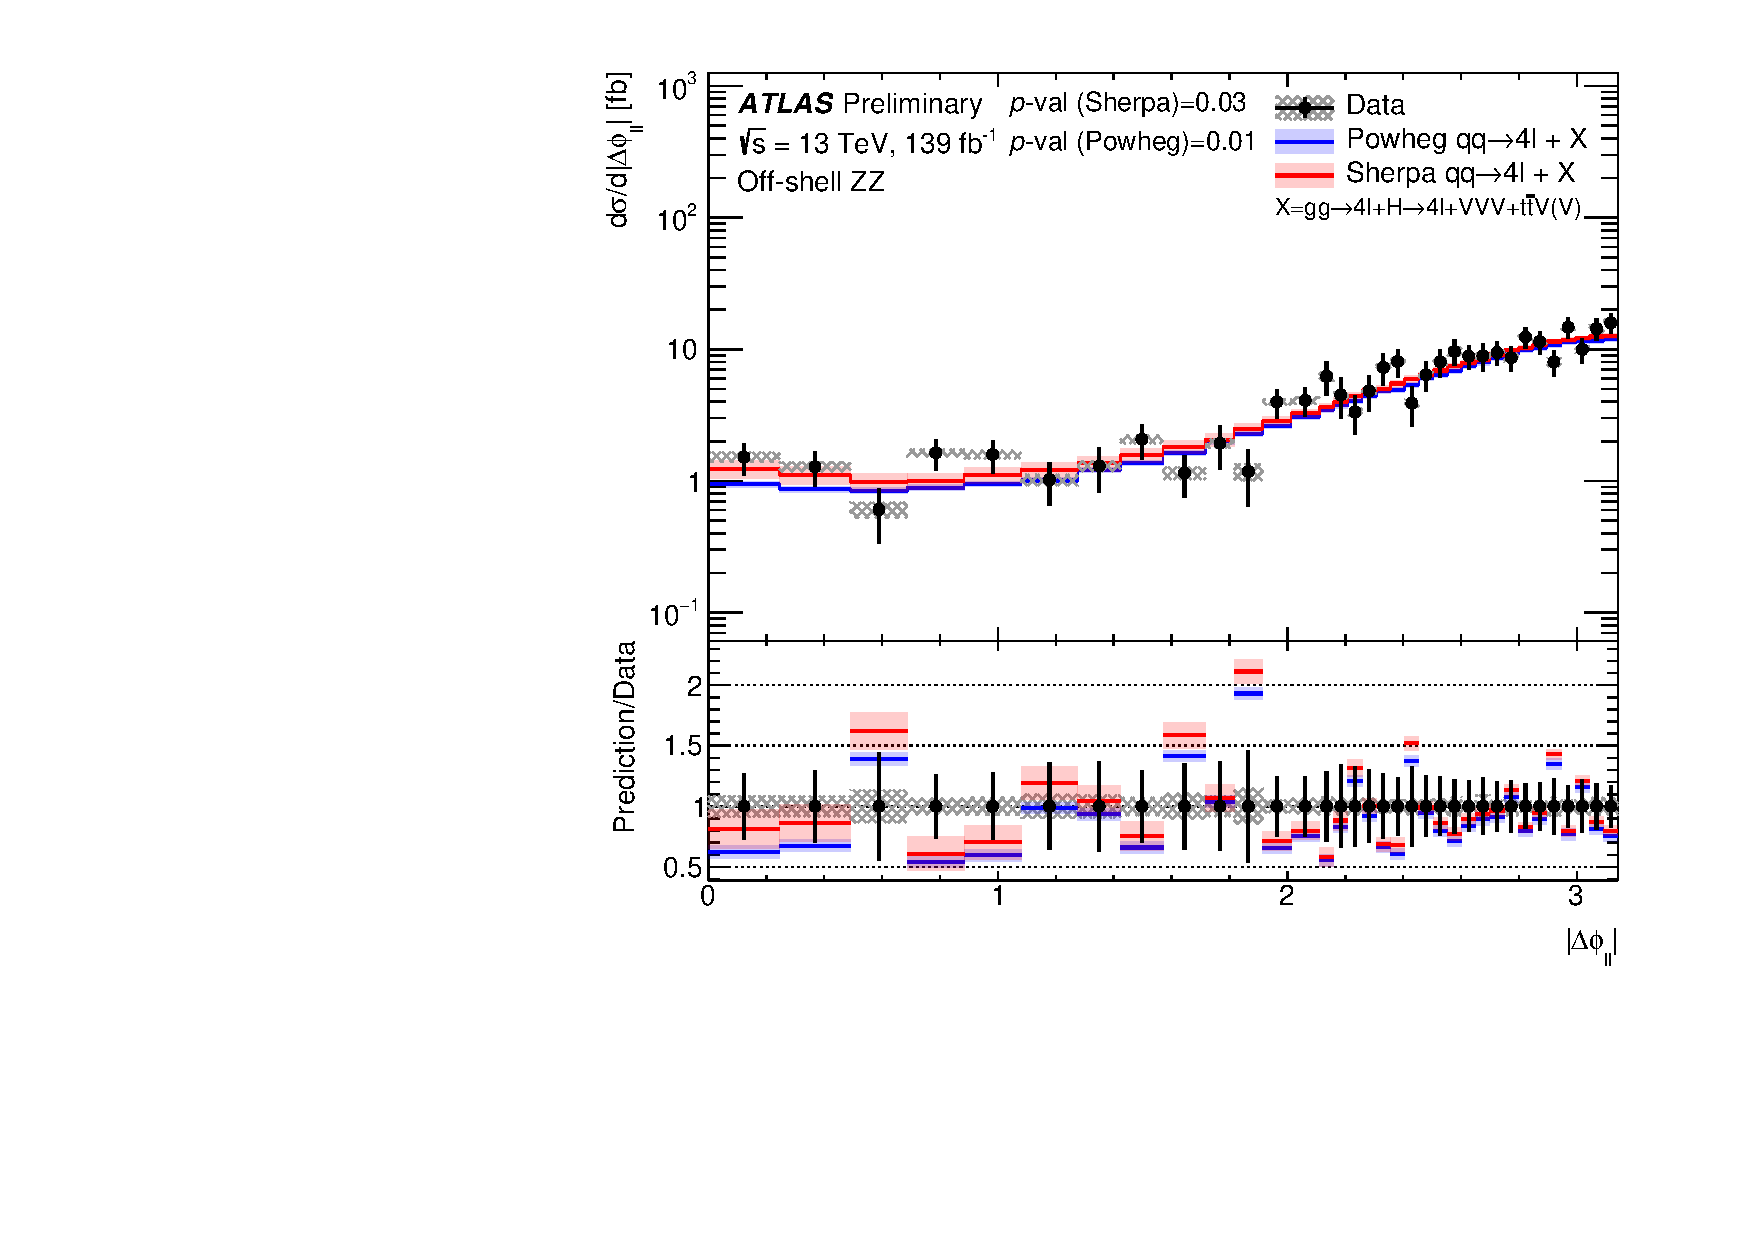
\includegraphics[width=.95\linewidth]{Figures/m4l/UnfoldedResults/Unfolded_Data_deltaPhiLeadingLeptons_m4loffshell.pdf}  \caption{Off-shell $\Z\Z$ region}\label{fig:sub-third}
    \end{subfigure}
    \begin{subfigure}{.49\textwidth}\centering
      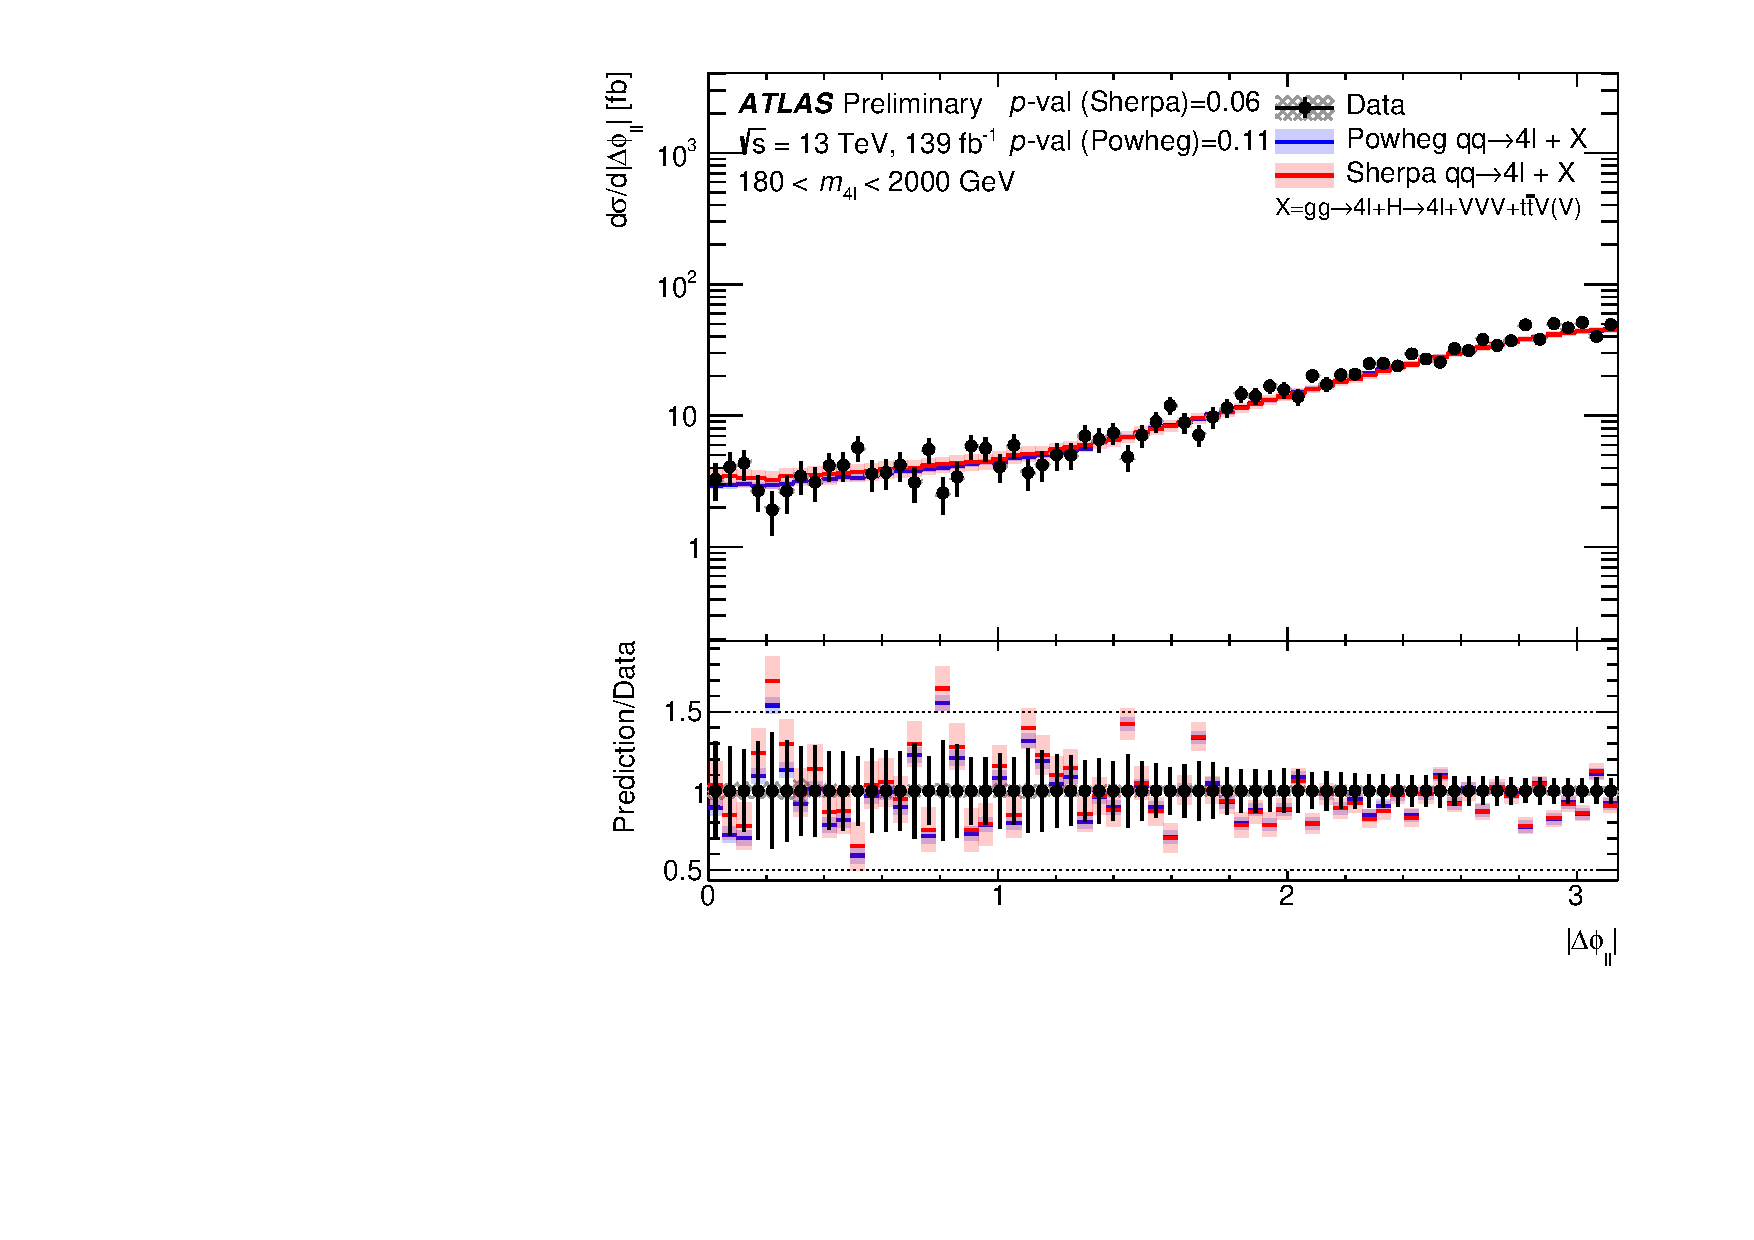
\includegraphics[width=.95\linewidth]{Figures/m4l/UnfoldedResults/Unfolded_Data_deltaPhiLeadingLeptons_m4l180-2000.pdf}  \caption{On-shell $\Z\Z$ region}\label{fig:sub-fourth}
    \end{subfigure}
    \caption{Differential cross-section as a function of \dPhill{} in the four
        \mFourL{} regions. The measured data (black points) are  compared with the SM prediction using either \SHERPA{} (red, with red hashed band for the uncertainty) or \POWHEG{} + \pythia{} (blue, with blue hashed band for the uncertainty) to model the \qqFourL{} contribution. The error bars on the data points give the total uncertainty and the grey hashed band gives the systematic uncertainty. \Pvalue{} The  lower panel shows the ratio of the SM predictions to the data.}
    \label{fig:dPhill_m4l}
\end{figure}

%% deltaPhiPairs vs m4l
\begin{figure}[H]
    \begin{subfigure}{.49\textwidth}\centering
      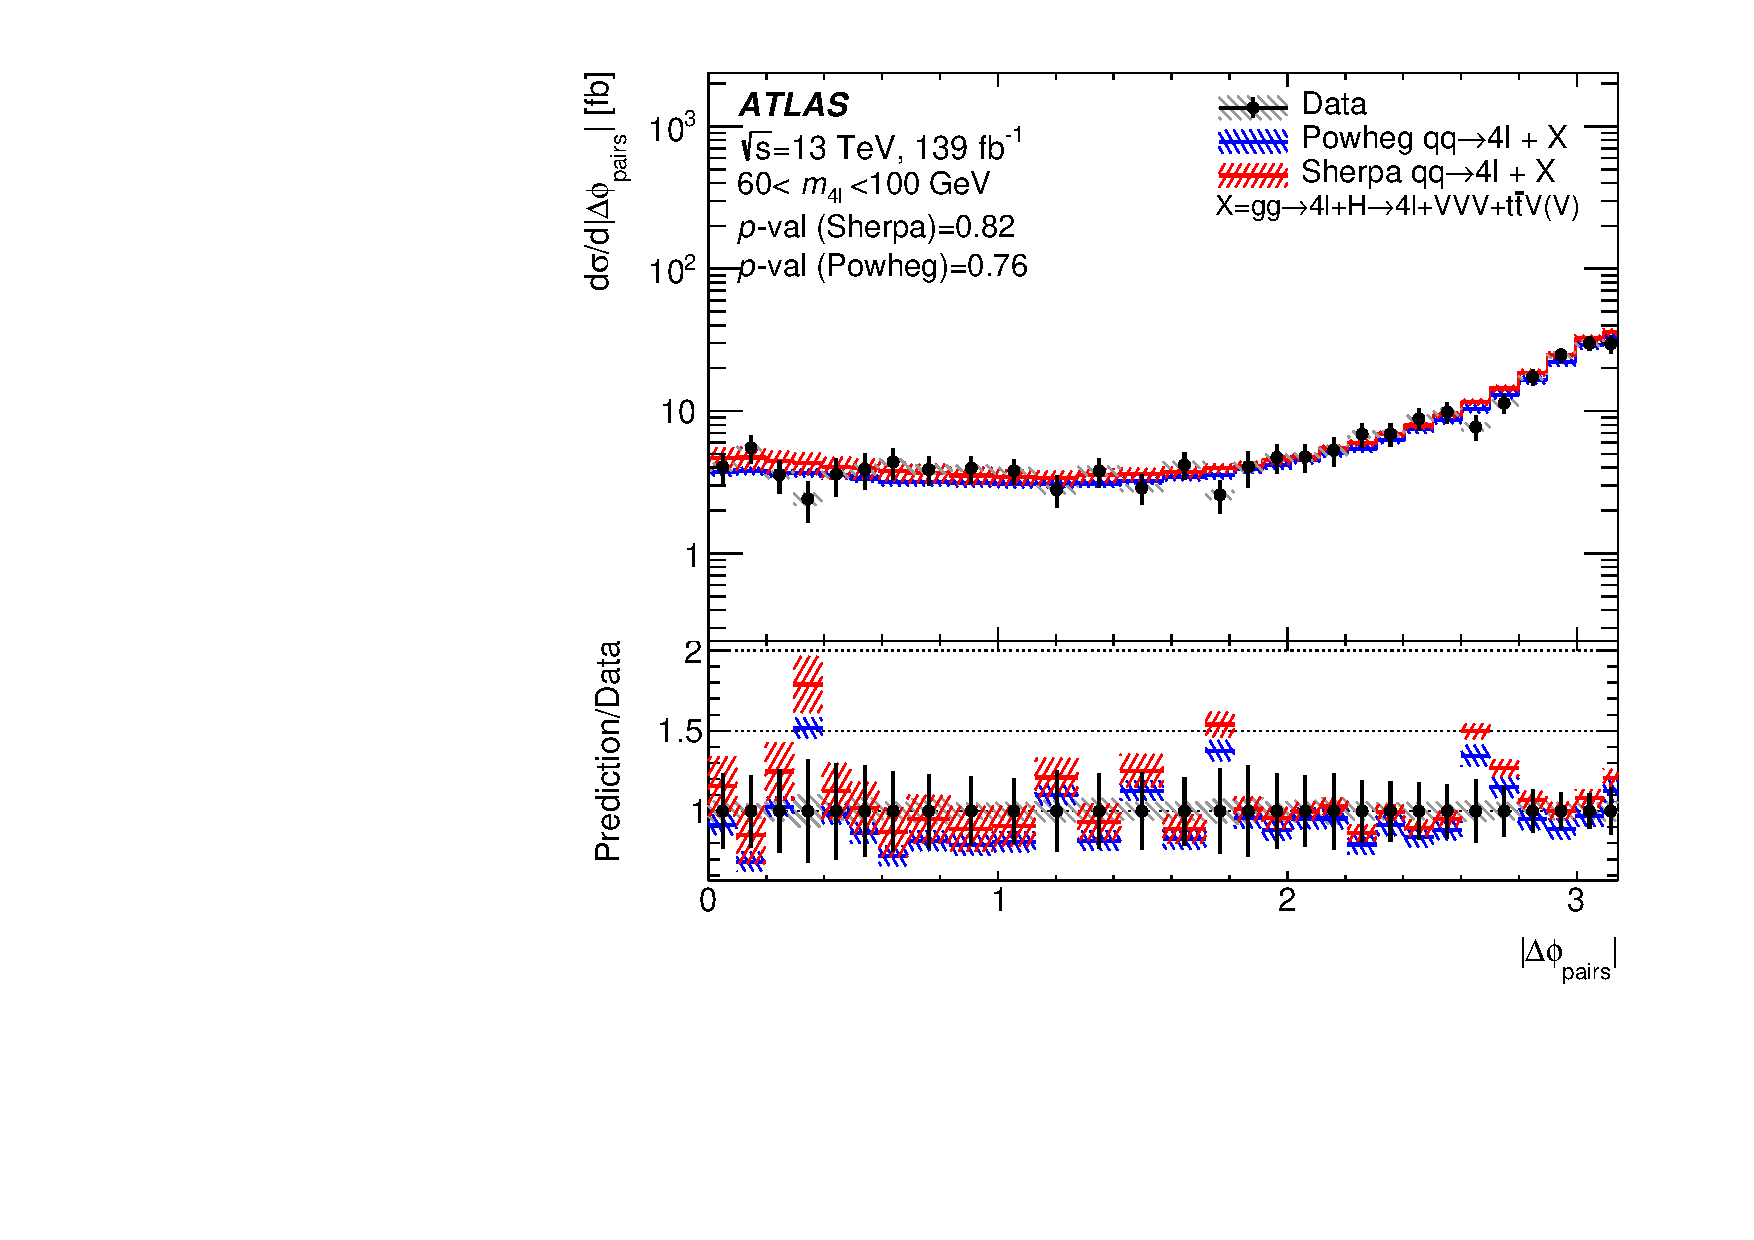
\includegraphics[width=.95\linewidth]{Figures/m4l/UnfoldedResults/Unfolded_Data_deltaPhiPairs_m4l60-100.pdf}\caption{\ZFourL \ region}\label{fig:sub-first}
    \end{subfigure}
    \begin{subfigure}{.49\textwidth}\centering
      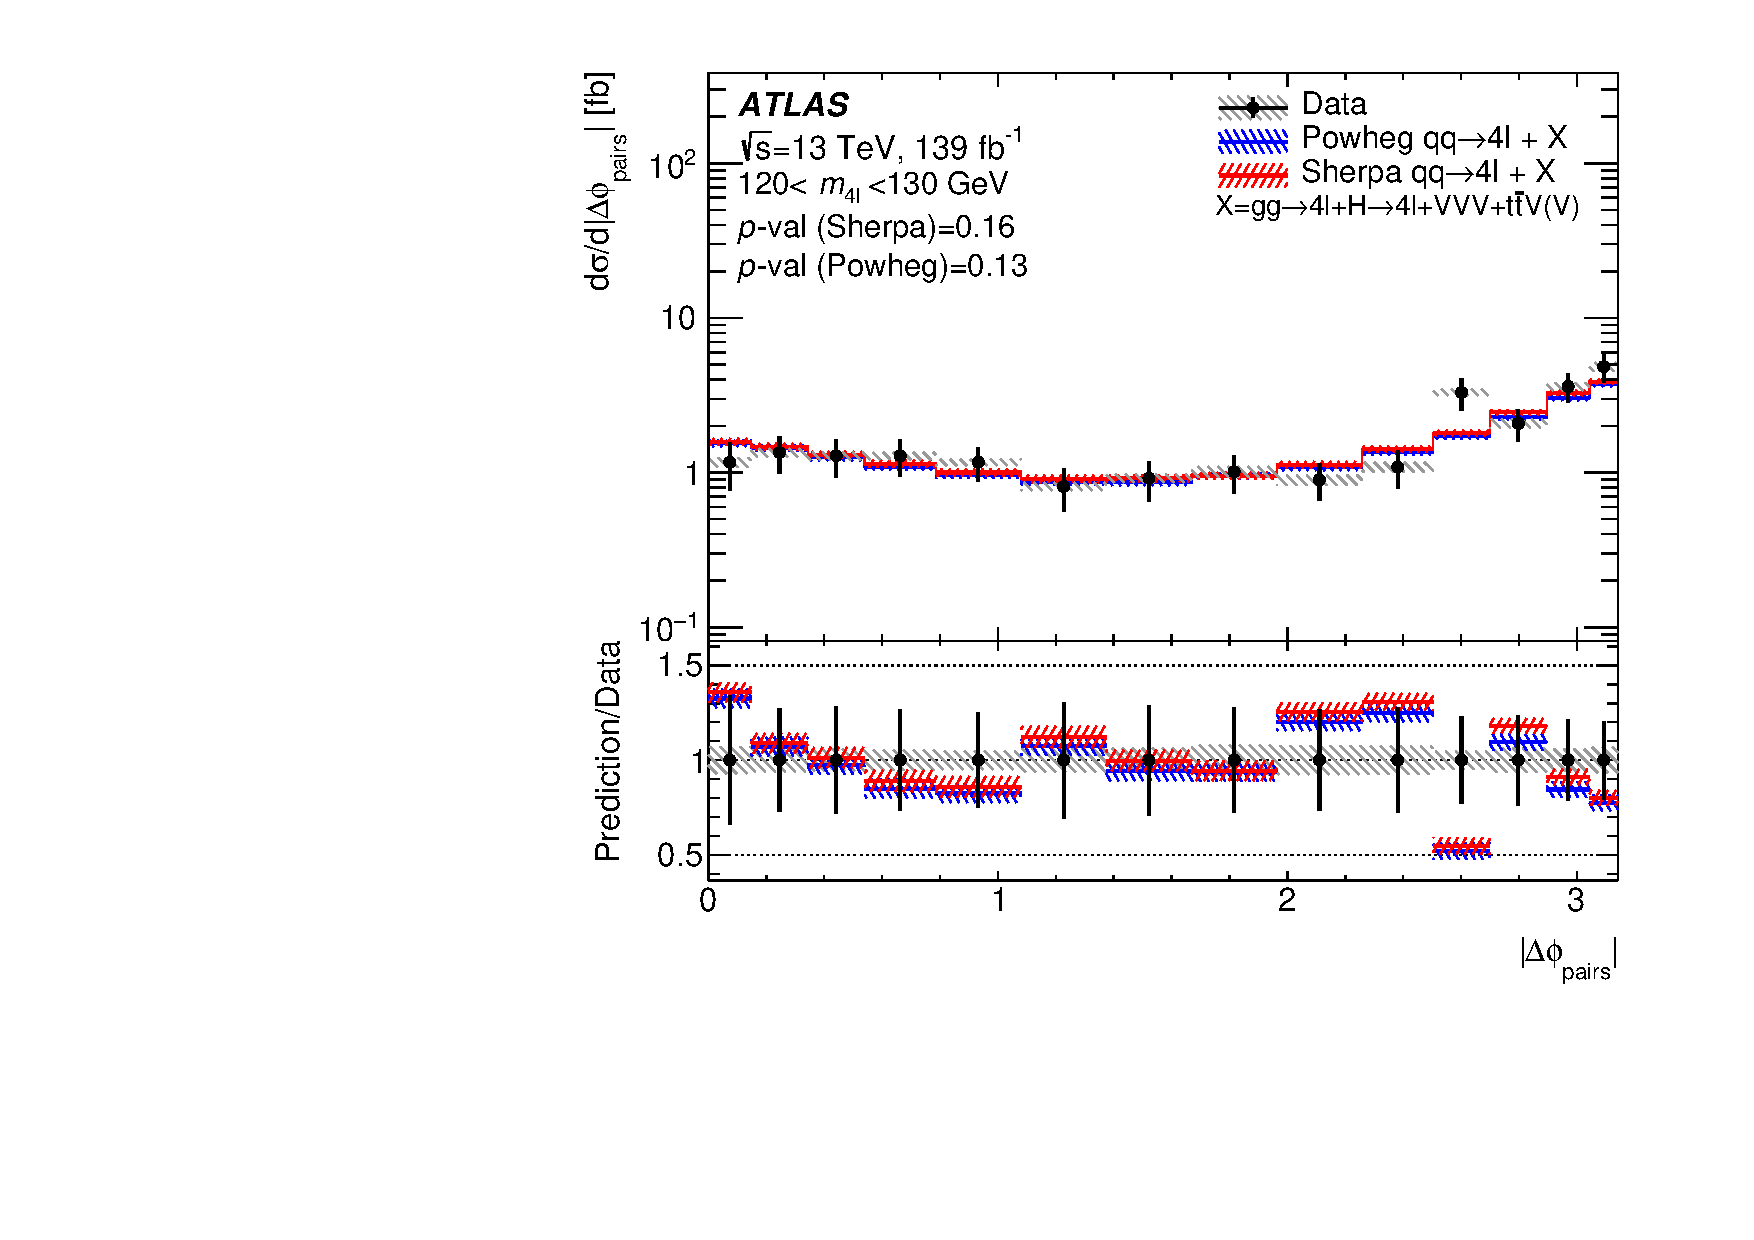
\includegraphics[width=.95\linewidth]{Figures/m4l/UnfoldedResults/Unfolded_Data_deltaPhiPairs_m4l120-130.pdf} \caption{\HFourL \ region}\label{fig:sub-second}
    \end{subfigure}
    \begin{subfigure}{.49\textwidth}\centering
      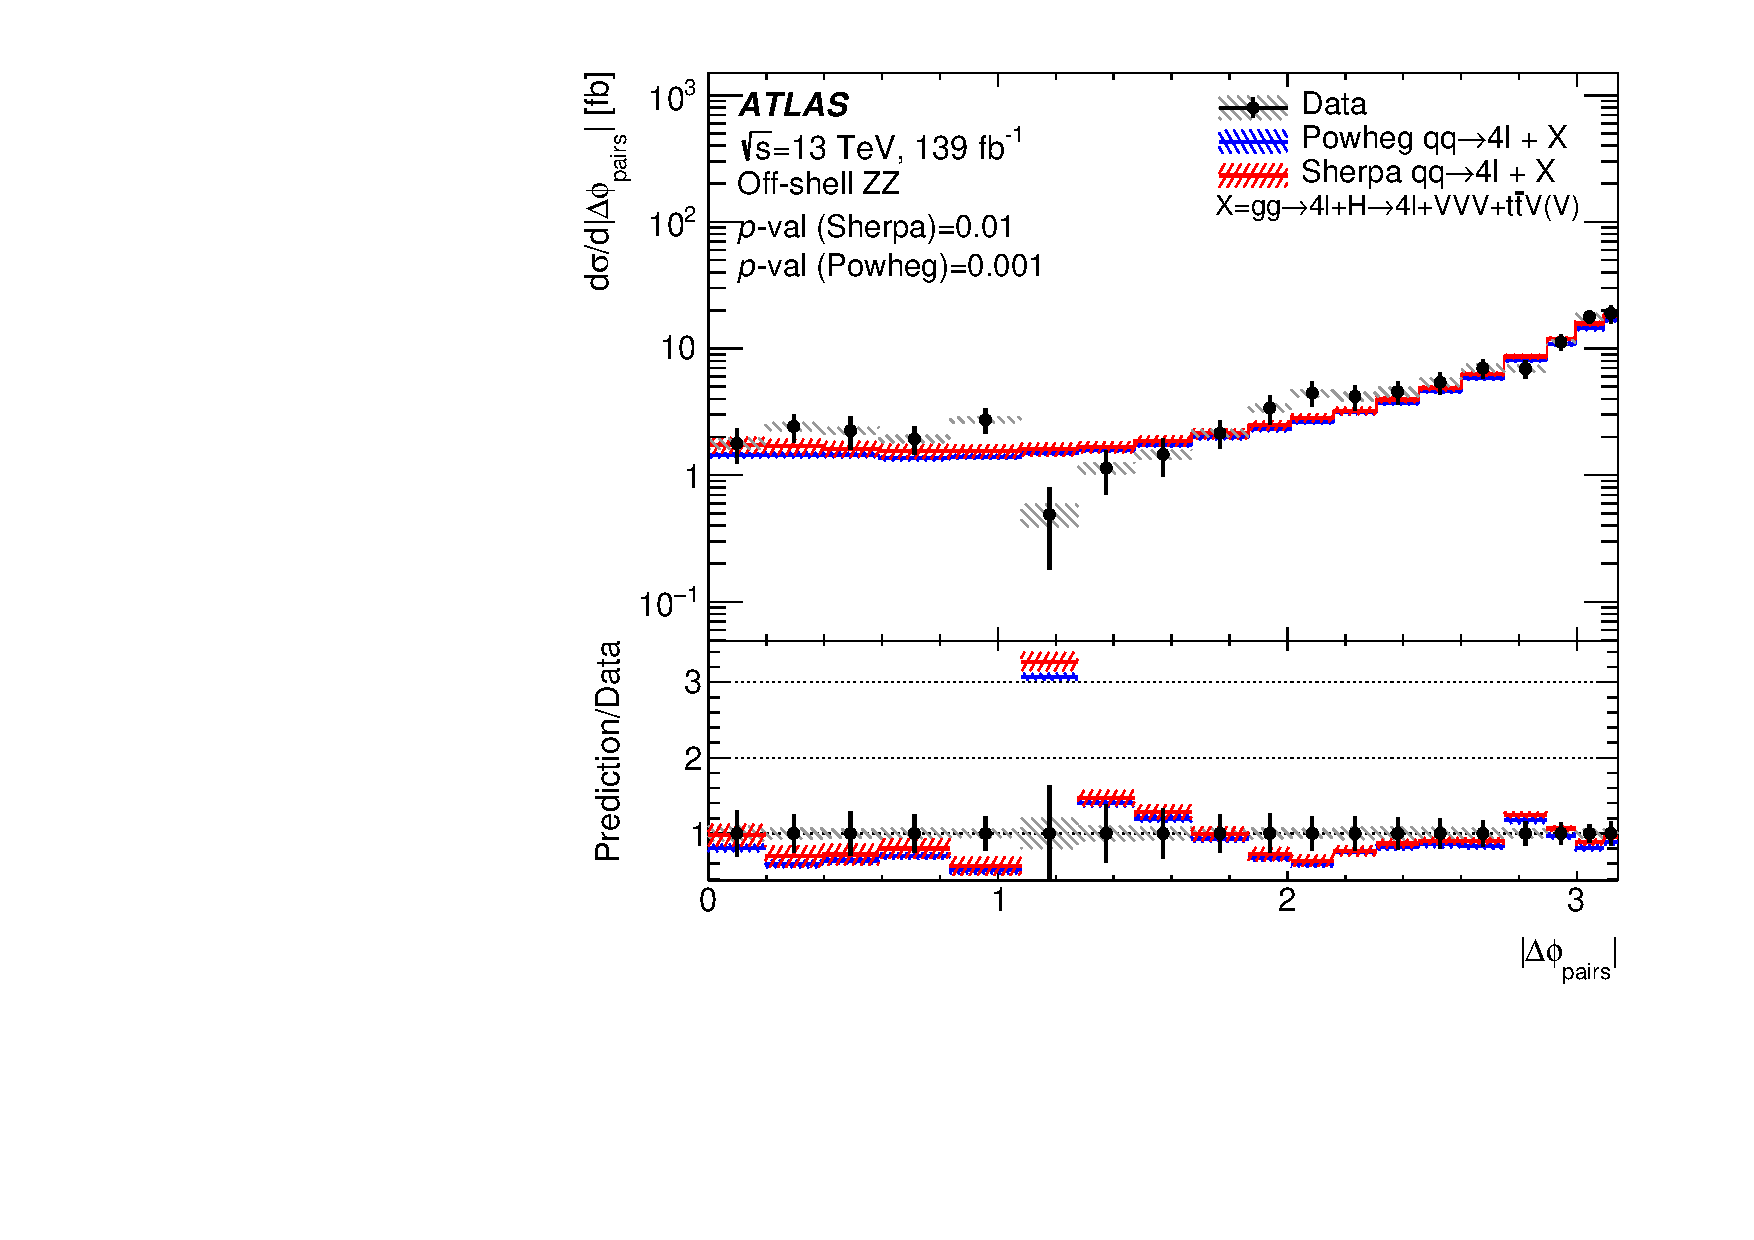
\includegraphics[width=.95\linewidth]{Figures/m4l/UnfoldedResults/Unfolded_Data_deltaPhiPairs_m4loffshell.pdf}  \caption{Off-shell $\Z\Z$ region}\label{fig:sub-third}
    \end{subfigure}
    \begin{subfigure}{.49\textwidth}\centering
      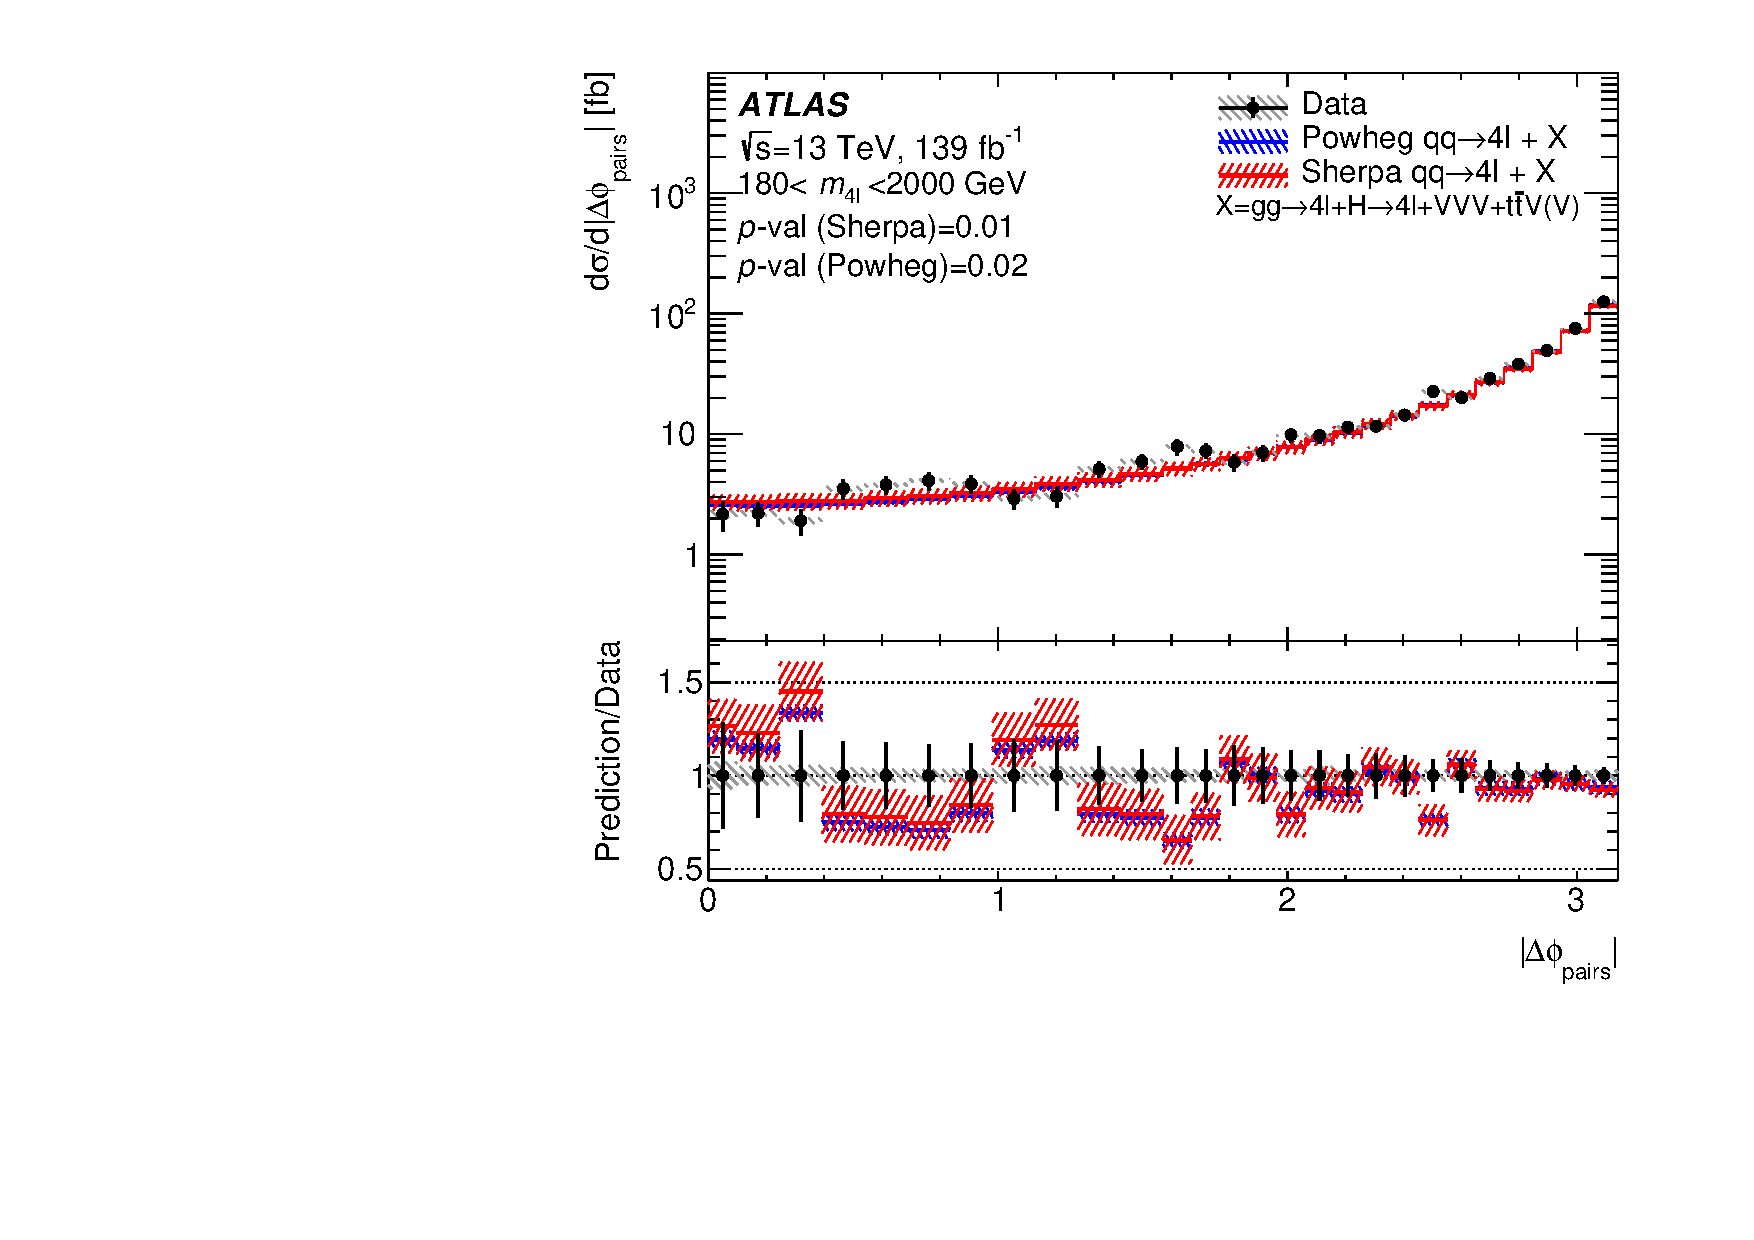
\includegraphics[width=.95\linewidth]{Figures/m4l/UnfoldedResults/Unfolded_Data_deltaPhiPairs_m4l180-2000.pdf}  \caption{On-shell $\Z\Z$ region}\label{fig:sub-fourth}
    \end{subfigure}
    \caption{Differential cross-section as a function of \dPhiPairs{} in the four
        \mFourL{} regions. The measured data (black points) are  compared with the SM prediction using either \SHERPA{} (red, with red hashed band for the uncertainty) or \POWHEG{} + \pythia{} (blue, with blue hashed band for the uncertainty) to model the \qqFourL{} contribution. The error bars on the data points give the total uncertainty and the grey hashed band gives the systematic uncertainty. \Pvalue{} The  lower panel shows the ratio of the SM predictions to the data.}
    \label{fig:dPhiPairs_m4l}
\end{figure}

%% deltaYPairs vs m4l
\begin{figure}[H]
    \begin{subfigure}{.49\textwidth}\centering
      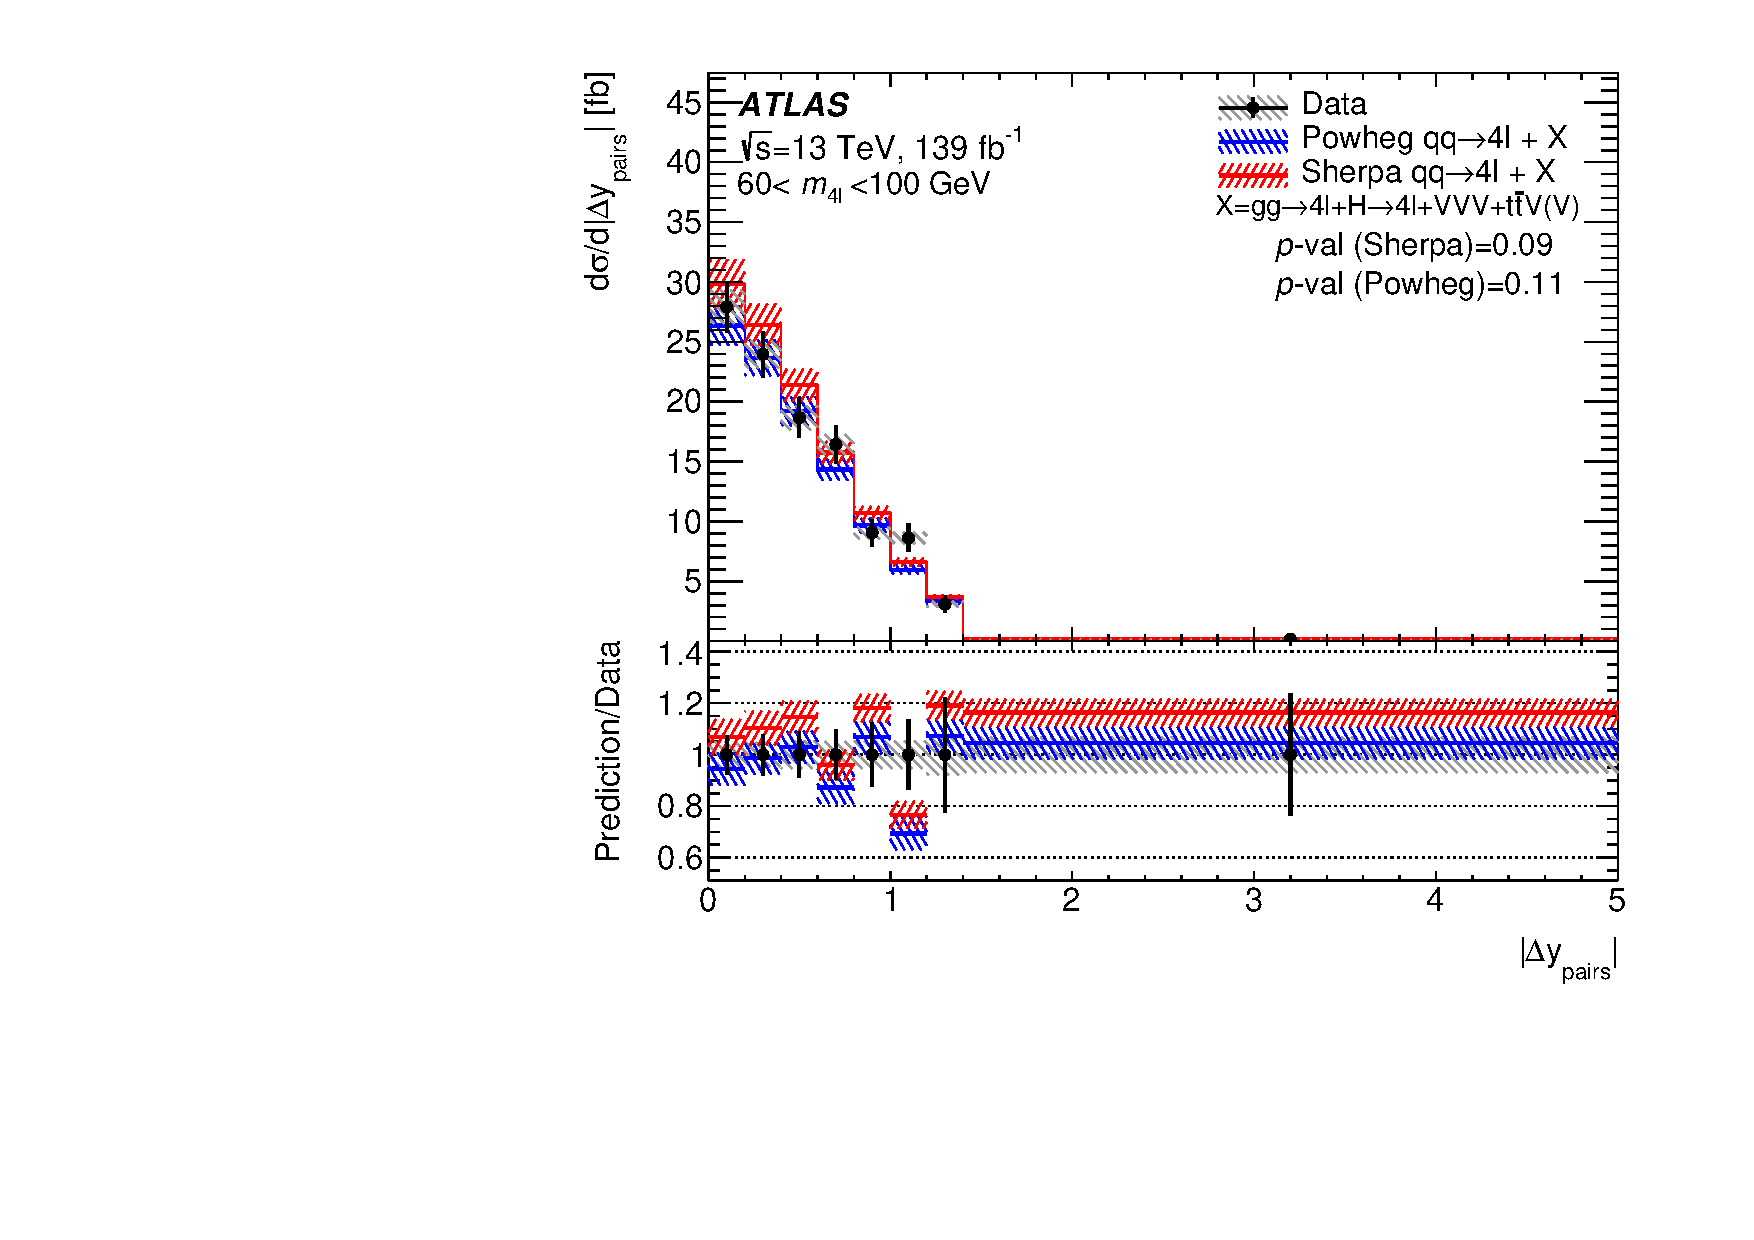
\includegraphics[width=.95\linewidth]{Figures/m4l/UnfoldedResults/linY_Unfolded_Data_deltaYPairs_m4l60-100.pdf}\caption{\ZFourL \ region}\label{fig:sub-first}
    \end{subfigure}
    \begin{subfigure}{.49\textwidth}\centering
      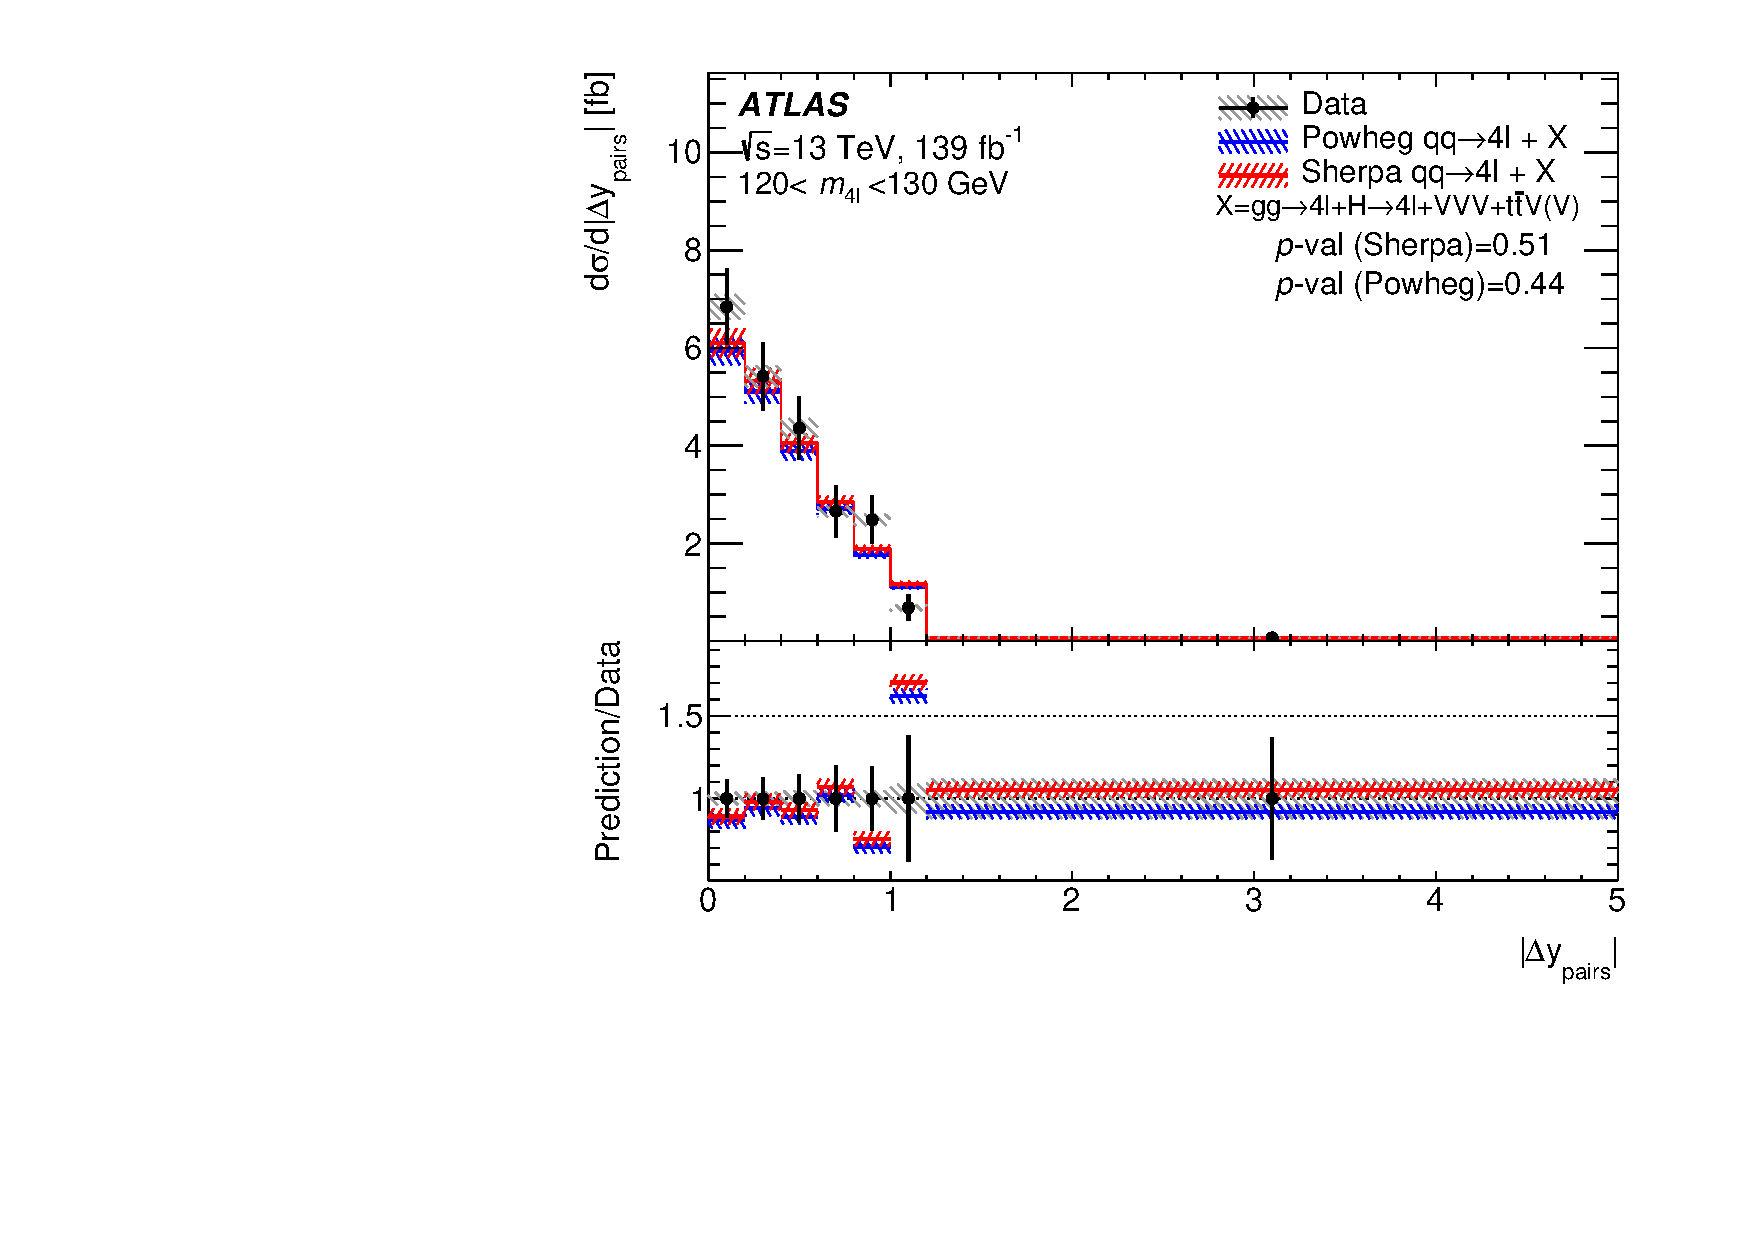
\includegraphics[width=.95\linewidth]{Figures/m4l/UnfoldedResults/linY_Unfolded_Data_deltaYPairs_m4l120-130.pdf} \caption{\HFourL \ region}\label{fig:sub-second}
    \end{subfigure}
    \begin{subfigure}{.49\textwidth}\centering
      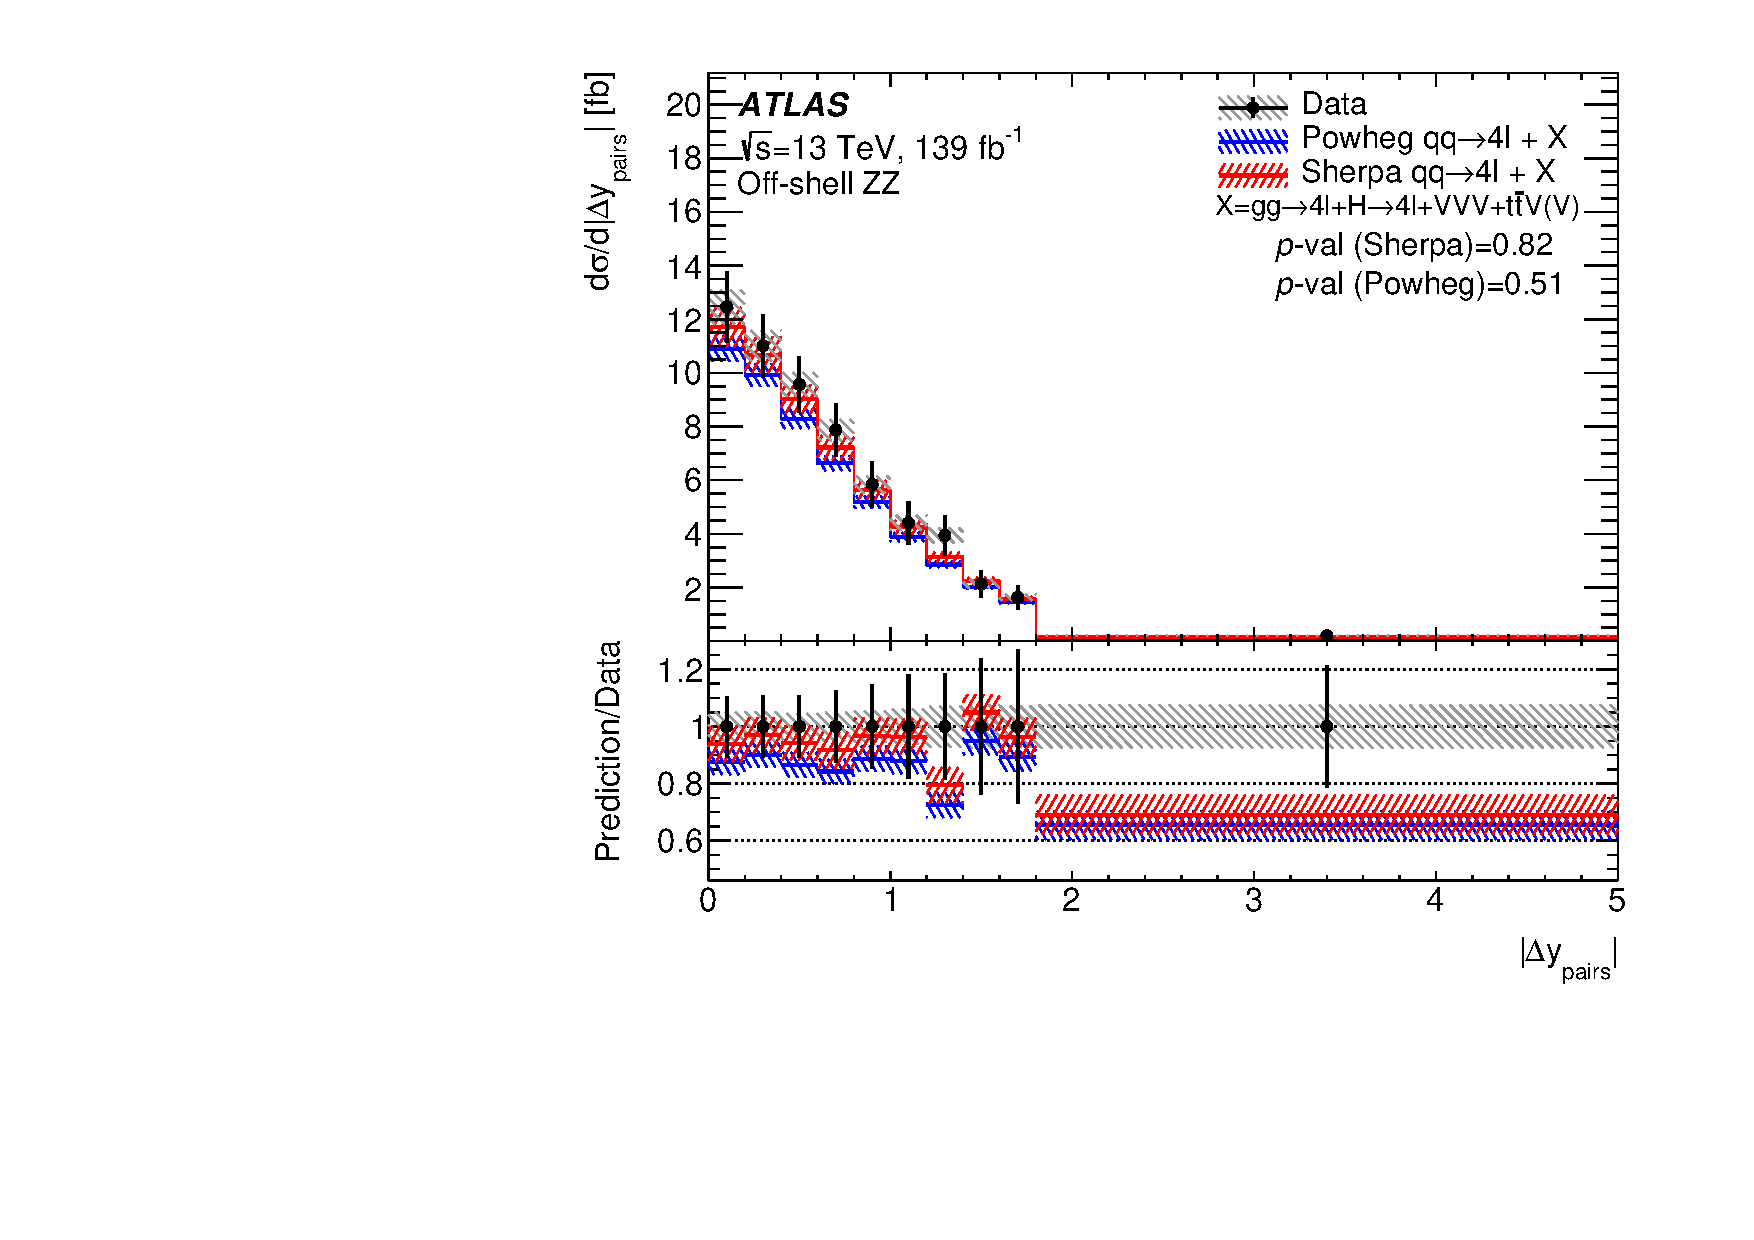
\includegraphics[width=.95\linewidth]{Figures/m4l/UnfoldedResults/linY_Unfolded_Data_deltaYPairs_m4loffshell.pdf}  \caption{Off-shell $\Z\Z$ region}\label{fig:sub-third}
    \end{subfigure}
    \begin{subfigure}{.49\textwidth}\centering
      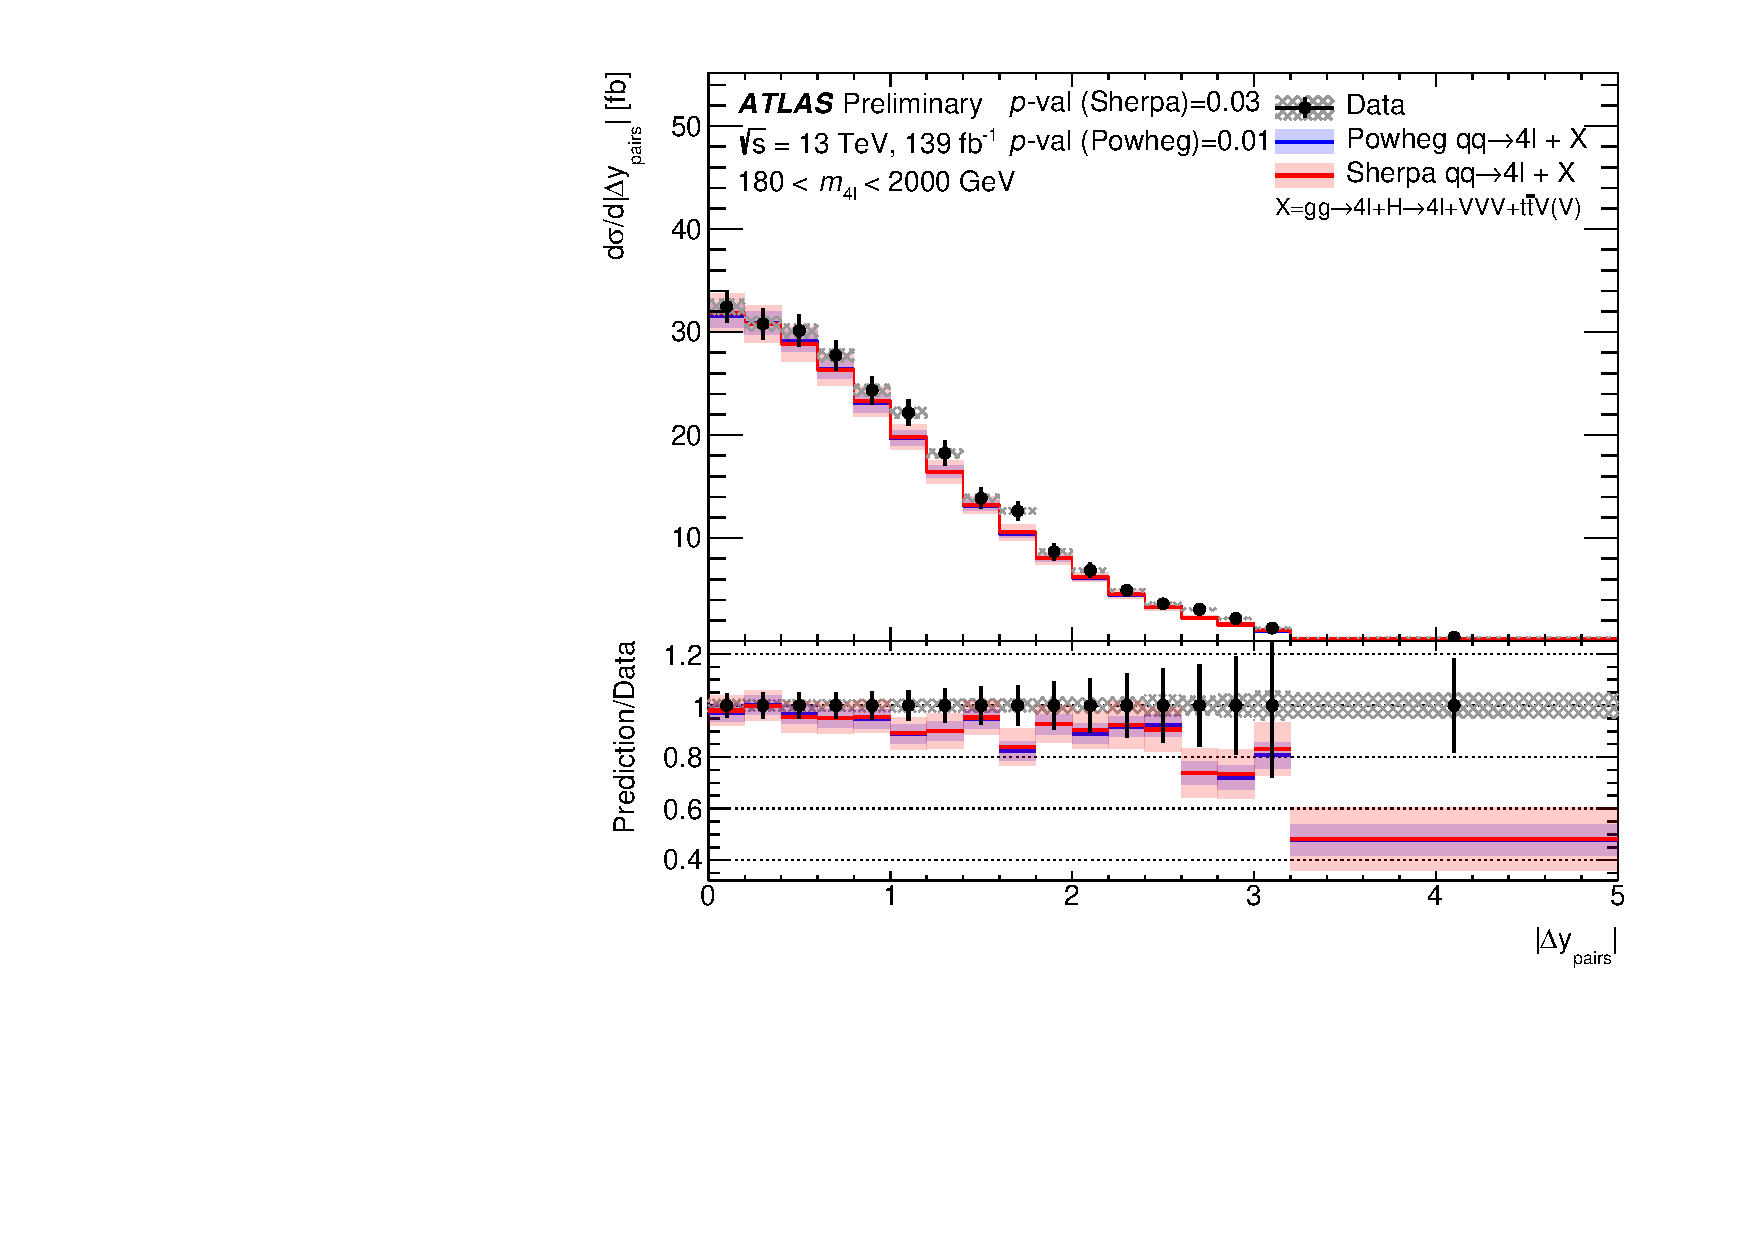
\includegraphics[width=.95\linewidth]{Figures/m4l/UnfoldedResults/linY_Unfolded_Data_deltaYPairs_m4l180-2000.pdf}  \caption{On-shell $\Z\Z$ region}\label{fig:sub-fourth}
    \end{subfigure}
    \caption{Differential cross-section as a function of \dYPairs{} in the four
        \mFourL{} regions. The measured data (black points) are  compared with the SM prediction using either \SHERPA{} (red, with red hashed band for the uncertainty) or \POWHEG{} + \pythia{} (blue, with blue hashed band for the uncertainty) to model the \qqFourL{} contribution. The error bars on the data points give the total uncertainty and the grey hashed band gives the systematic uncertainty. \Pvalue{} The  lower panel shows the ratio of the SM predictions to the data.}
    \label{fig:dYPairs_m4l}
\end{figure}